\documentclass[a4paper, 11pt]{article}

\setlength{\oddsidemargin}{0in}
\setlength{\textwidth}{6.5in}
\setlength{\topmargin}{-0.5in}
\setlength{\textheight}{9in}

\usepackage[T1]{fontenc}
\usepackage[utf8]{inputenc}  % Для LaTeX
\usepackage[T2A]{fontenc}   
\usepackage[english, russian]{babel}
\usepackage[normalem]{ulem}  
\usepackage{amsmath,amssymb}
\usepackage{graphicx}
\usepackage{caption}
\usepackage{subcaption}
\usepackage{color}
\usepackage{dcolumn}
\usepackage{bm}
\usepackage{float}



\newcommand{\expnumber}[2]{{#1}\mathrm{e}{#2}}
\newcommand{\doublenorm}[1]{\left\lVert #1 \right\rVert}

\usepackage{amsmath}
\usepackage{amssymb}
\usepackage{amsthm}
% \usepackage[cal=boondox]{mathalfa} % Подключает каллиграфические шрифты
\usepackage{pdfpages}
\usepackage{multirow}
\usepackage{booktabs} % Для более красивых таблиц
\usepackage{multirow}
\usepackage{booktabs}
\usepackage{amsmath}


\usepackage[colorlinks=true, linkcolor=black, citecolor=black, urlcolor=black]{hyperref}

\setcounter{tocdepth}{2}

\newcommand{\SSA}{\textbf{SSA}}
\newcommand{\GSSA}{\textbf{GSSA}}
\newcommand{\CISSA}{\textbf{CiSSA}}
\newcommand{\MSSA}{\textbf{MSSA}}
\newcommand{\FSSA}{\textbf{FSSA}}
\newcommand{\DSSA}{\textbf{2d-SSA}}
\newcommand{\TS}{\mathsf{X}}


\newcommand{\MSE}{\textbf{MSE}}


\newtheorem{definition}{Определение} % задаём выводимое слово (для определений)
\newtheorem{theorem}{Теорема} % задаём выводимое слово (для определений)
\newtheorem{comment}{Замечание} % задаём выводимое слово (для определений)

%\usepackage{fleqn}
\pdfoutput=1
\pdfcompresslevel=0

%##################


\date{}
\begin{document}

%\documentclass[specialist,
               substylefile = spbu_report.rtx,
               subf,href,colorlinks=true, 12pt]{disser}

\usepackage[a4paper,
            mag=1000, includefoot,
            left=3cm, right=1.5cm, top=2cm, bottom=2cm, headsep=1cm, footskip=1cm]{geometry}
\usepackage[T2A]{fontenc}
\usepackage[cp1251]{inputenc}
\usepackage[english,russian]{babel}
\usepackage{graphicx}
\usepackage{epsfig}
\usepackage{amsfonts}
\usepackage{amssymb}
\usepackage{amsmath}
\usepackage[update,prepend]{epstopdf}
\usepackage{amsfonts}
\usepackage{subcaption}
\ifpdf\usepackage{epstopdf}\fi

\usepackage{adjustbox}
\usepackage{amsthm}
\usepackage{indentfirst}
\newtheorem{definition}{�����������} % ����� ��������� ����� (��� �����������)


% ����� � ������� � �������� ����������� ����� �������� �����������
%\setcitestyle{semicolon}

% ������������ ���������� ���������� ��� ��������
\let\vec=\mathbf

\newcommand{\SSA}{\textbf{SSA}}

% �������� ��������� � ����������
\setcounter{tocdepth}{2}

\graphicspath{{fig/}}

%----------------------------------------------------------------
\begin{document}

%
% ��������� ���� �� ������� �����
%
% �������� �����������
\institution{%
    �����-������������� ��������������� �����������\\
    ���������� ���������� � �����������
}

\title{����� �� ������� �������� 3 (������-����������������� ������)}

% ����
\topic{����������� ������ ������� ������������ ������� ��� ������� ��������� �����: Circulant SSA}

% �����
\author{����������� ������� ���������}
\group{������ 21.�04-��}
    
% ������� ������������
\sa       {��������� ���� ����������\\%
           ������� ��������������� �������������}
\sastatus {�.\,�.-�.\,�., ���.}

% ����� � ���
\city{�����-���������}
\date{\number\year}

\maketitle



\bibliographystyle{ugost2008}


\end{document}


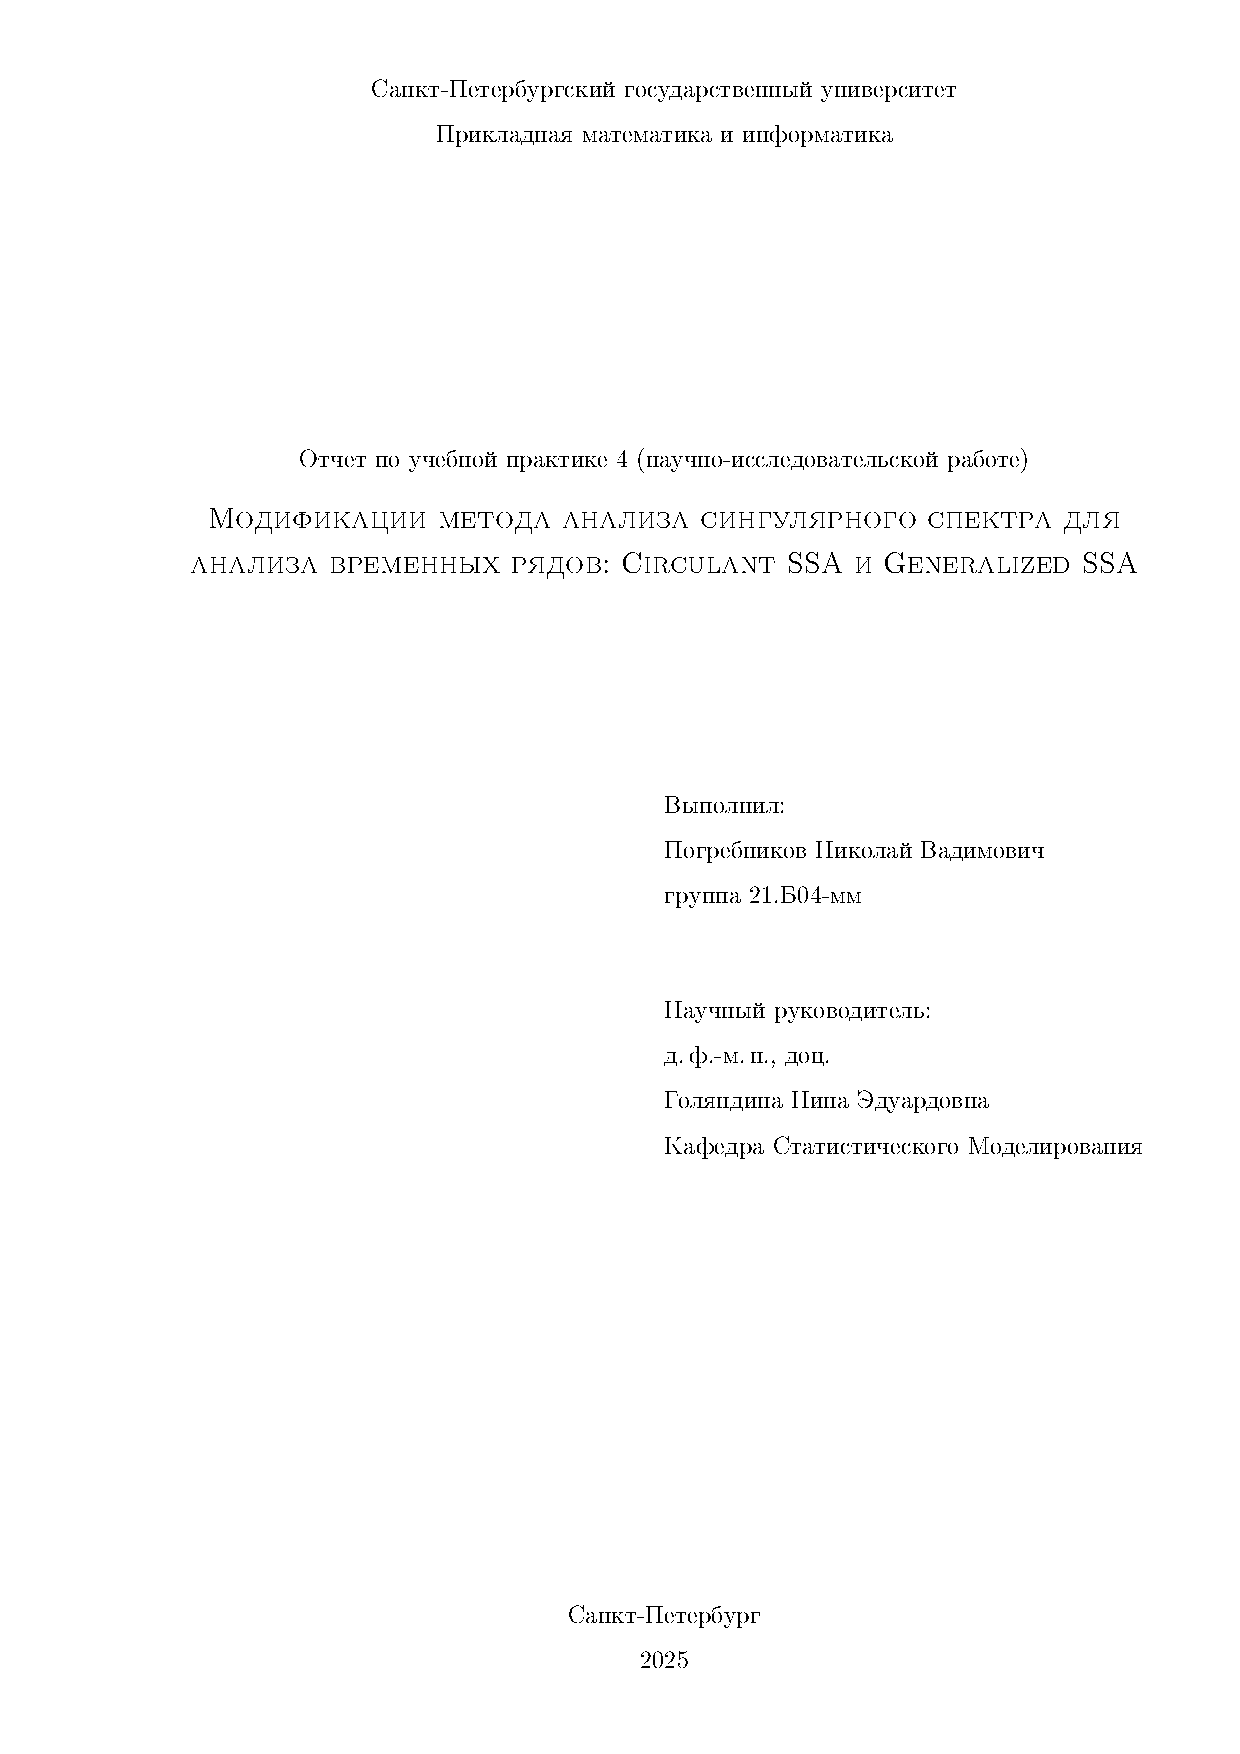
\includepdf[pages=-]{../Title/report.pdf}

\tableofcontents
\noindent
\textbf{11\textit{} \space Список литературы}

\newpage

\section{Введение}


Временные ряды представляют собой упорядоченную последовательность данных, собранных или измеренных в хронологическом порядке. Они играют ключевую роль в анализе и прогнозировании различных явлений в таких областях, как экономика, финансы, климатология и медицина. Понимание эволюции этих явлений во времени критично для выявления тенденций, циклов и аномалий.

Для уточнения терминологии, следует отметить, что \textbf{временной ряд длины \( N \)} представляет собой упорядоченную конечную последовательность значений, которая записывается как \( \TS = (x_1, \dots, x_{N}) \), где \( N > 2 \), $x_i \in \mathbb{R}$. Одним из основных аспектов анализа временных рядов является разделение их на составляющие компоненты. Среди таких компонентов важными являются \textbf{тренд}, который отражает медленно изменяющуюся долгосрочную динамику ряда, и \textbf{сезонность}, представляющая собой периодические колебания, вызванные повторяющимися факторами, такими как климатические или экономические циклы.

Для эффективного анализа и понимания структуры временных рядов разработаны различные методы, позволяющие разделить ряд на его компоненты. Существует два вида разделимости: \textbf{точная разделимость}, которая характеризует способность метода точно выделять отдельные компоненты ряда, и \textbf{асимптотическая разделимость}, которая описывается следующим образом:

\begin{definition}
	\label{def:asymp}
	Есть метод разделения ряда на компоненты с параметрами \( \Theta \), ряд \( \TS = \TS^{(1)} + \TS^{(2)} \). Существуют такой фиксированный набор параметров \( \hat{\Theta} \) и последовательность \( L = L(N) \), \( N \rightarrow \infty \), что при разделении ряда на компоненты этим методом, \( \hat{\TS}^{(1)} \) является оценкой \( \TS^{(1)} \), при этом, \( \mathrm{MSE}\left(\TS^{(1)}, \hat{\TS}^{(1)}\right) \rightarrow 0 \), где \( \mathrm{MSE} \) --- среднеквадратическая ошибка. Тогда ряды \( \TS^{(1)} \) и \( \TS^{(2)} \) называются асимптотически \( L(N) \)-разделимыми данным методом.
\end{definition}

\begin{comment}
$\hat \TS^{(2)} = \TS - \hat \TS^{(1)}$ является оценкой для $\TS^{(2)}$, выполнено
$\mathrm{MSE}\left(\TS^{(2)}, \hat \TS^{(2)}\right) \rightarrow 0$.
\end{comment}

Методы разделения временных рядов играют ключевую роль в выделении тренда, сезонности и других структурных компонентов, что позволяет глубже понять и моделировать временные зависимости.


В данной работе будут рассмотрены следующие постановки задачи разделения временных рядов:
\begin{enumerate}
	\item \label{item:freq} Разделение временного ряда на компоненты, соответствующие определенным частотным диапазонам;
	\item \label{item:general} Разделение временного ряда на компоненты без привязки к частотным характеристикам, то есть в их исходном виде.
\end{enumerate}


Анализ сингулярного спектра ($\SSA$ \cite{golyandina2001analysis}) --- метод, целью которого является разложение оригинального ряда на сумму небольшого числа интерпретируемых компонентов, таких как медленно изменяющаяся тенденция (тренд), колебательные компоненты (сезонность) и шум. Позволяет решать как задачу в формулировке \ref{item:freq}, так и её обобщение, представленное в \ref{item:general}. При этом, базовый алгоритм метода $\SSA$ не требует стационарности ряда, знания модели тренда, а также сведений о наличии в ряде периодиках, а за счет своего адаптивного базиса позволяет подстраиваться под любой входной ряд.

В данном исследовании рассматриваются модификации $\SSA$, предложенные другими авторами, а именно, $\GSSA$ \cite{gu2024generalized} и $\CISSA$ \cite{bogalo2020}, $\FSSA$ \cite{haghbin2019functionalsingularspectrumanalysis}.


$\GSSA$ отличается от базового $\SSA$ тем, что он добавляет веса на определенном этапе алгоритма $\SSA$. В некоторых случаях это может оказаться полезным, в других --- повлиять на разделимость в худшую сторону.
Это исследование раскрывает смысловую ценность $\GSSA$ с точки зрения линейных фильтров и отмечает ситуации, где такой алгоритм предпочтительнее стандартного $\SSA$.


В алгоритме $\CISSA$ предложено решение задачи разделения временного ряда на заранее известные компоненты (задача в постановке \ref{item:freq}), отвечающие конкретным периодикам. За счет этого можно автоматически группировать компоненты по частотам, однако именно поэтому алгоритм лишается адаптивности, которая имеется в $\SSA$.

$\FSSA$ рассматривается как многомерная модификация $\SSA$, основанная на скрещивании подходов функционального анализа и теории $\SSA$.

Целью работы является описание модификаций в контексте теории $\SSA$ и на этой основе сравнение методов по теоретическим свойствам и численно.

Далее кратко опишем структуру работы. В разделе \ref{sec:ssa} рассматривается базовый метод $\SSA$ и его ключевые свойства. В секциях \ref{sec:gssa}, \ref{sec:compare_ssa_gssa} показан алгоритм $\GSSA$ и проведено сравнение с $\SSA$. В следующих разделах \ref{sec:cissa}, \ref{sec:comparison_cissa} представлен метод $\CISSA$, также с описанием его основных характеристик и проведено сравнение с $\SSA$. Раздел \ref{sec:multidimensional_ssa} посвящен модификациям $\MSSA$ и $\DSSA$ базового $\SSA$ для использования его в многомерном случае. Затем в секциях \ref{sec:fssa}, \ref{sec:compare_fssa_ssa} рассматривается алгоритм $\FSSA$ и его сравнение с $\DSSA$, $\MSSA$.  В заключительной секции \ref{sec:concl} подведены основные итоги исследования.

В предыдущей научно-исследовательской работе было проведено сравнение алгоритмов $\SSA$ и $\CISSA$ с точки зрения их способности к разделению временных рядов. Для этого была написана реализация алгоритма $\CISSA$ на языке программирования R, проведено сравнение с методами $\SSA$ и преобразованием Фурье. Кроме того, была создана реализация алгоритма $\GSSA$ на языке R, и проведено сравнение его достоинств и недостатков с методом $\SSA$.

В рамках текущего исследования было продолжено изучение указанных методов. Конкретнее, было рассмотрено влияние конкретной точки во времени на ошибку временного ряда для методов $\GSSA$ и $\SSA$. Кроме того, список примеров для $\CISSA$ был дополнен анализом сумм экспоненциально-модулированных гармоник. А также были изучены практические применения метода $\CISSA$. Наконец, было проведено численное сравнение методов $\MSSA$, $\DSSA$ и $\FSSA$ с численной оценкой их эффективности.


\newpage

\section{Метод Singular spectrum analysis (SSA)}
\label{sec:ssa}


Рассмотрим базовый метод сингулярного спектрального анализа \cite{golyandina2001analysis}.

\subsection{Алгоритм метода SSA}

Пусть $N > 2$, вещественнозначный временной ряд
$\TS = (x_1, \dots, x_{N})$ длины $N$.
Базовый алгоритм $\SSA$ состоит из четырех шагов.

\subsubsection{Вложение}
Параметром этого шага является $L$ --- некоторое целое число (длина окна), $1 < L < N$. Строится $L$-траекторная матрица $\mathbf{X}$, состоящая из $K = N - L + 1$ векторов вложения:
\begin{equation}
	\label{eq:X}
	\mathcal{J} \left(\TS \right) = \mathcal{J}_{SSA} \left(\TS \right)=
	\mathbf{X} =
	\begin{pmatrix}
		x_1    & x_2     & x_3     & \dots  & x_{K}   \\
		x_2    & x_3     & x_4     & \dots  & x_{K+1} \\
		x_3    & x_4     & x_5     & \dots  & x_{K+2} \\
		\vdots & \vdots  & \vdots  & \ddots & \vdots  \\
		x_{L}  & x_{L+1} & x_{L+2} & \dots  & x_{N}
	\end{pmatrix}.
\end{equation}
Полезным свойством является то, что матрица $\mathbf{X}$ имеет одинаковые элементы на антидиагоналях. Таким образом, $L$-траекторная матрица является ганкелевой. $\mathcal{J}_{SSA}$ называется оператором вложения.

\subsubsection{Сингулярное разложение (SVD)}
Результатом этого шага является сингулярное разложение ($\mathbf{SVD}$) траекторной матрицы ряда.

Пусть $\mathbf{S} = \mathbf{X}\mathbf{X}^{\mathrm{T}}$,
$\lambda_1, \dots, \lambda_L$ --- собственные числа матрицы $\mathbf{S}$, взятые в неубывающем порядке, и
$U_1, \dots, U_L$ --- ортонормированная система собственных векторов, соответствующих собственным числам матрицы $\mathbf S$.

Определим $d = \max{ \{i: \lambda_i > 0 \}}$ и
$V_i = \mathbf{X}^{\mathrm{T}} U_i / \sqrt{\lambda_i}$.
Тогда сингулярным разложением называется представление матрицы в виде:
\begin{equation}
	\mathbf{X} = \mathbf{X}_1 + \dots + \mathbf{X}_d =
	\sum_{i = 1}^{d} \sqrt{\lambda_i} U_i V_{i}^{\mathrm{T}}\label{eq:1}.
\end{equation}

Набор $( \sqrt{\lambda_i}, U_i, V_{i}^{\mathrm{T}})$ называется $i$-й собственной тройкой разложения \eqref{eq:1}.

\subsubsection{Группировка}
На основе разложения \eqref{eq:1} производится процедура группировки, которая делит все множество индексов $\{1, \dots, d\}$ на $m$ непересекающихся подмножеств $I_1, \dots, I_m$. Это разбиение является параметром шага группировки.

Пусть $I = \{i_1, \dots, i_p\}$, тогда $\mathbf{X}_I =
	\mathbf{X}_{i_1} + \dots + \mathbf{X}_{i_p}$. Такие матрицы вычисляются для каждого $I = I_1, \dots, I_m$.
В результате получаются матрицы $\mathbf{X}_{I_1}, \dots, \mathbf{X}_{I_m}$. Тем самым разложение \eqref{eq:1} может быть записано в сгруппированном виде:
\begin{equation*}
	\mathbf{X} = \mathbf{X}_{I_1} + \dots + \mathbf{X}_{I_m}.
\end{equation*}

\subsubsection{Диагональное усреднение}
Пусть $\mathbf{Y}$ --- матрица размерности $L \times K$. $L^* = \min(L, K), \, K^* = \max(L,K)$. Диагональное усреднение переводит матрицу $\mathbf{Y}$ в временной ряд $g_1, \dots, g_{N} $:

\begin{equation*}
	g_{k}=
	\begin{cases}
		\frac{1}{k+1} \sum\limits_{m=1}^{k+1} y_{m,k-m+2}^{*}           &
		\text{для } 1 \leq k < L^*,                                       \\

		\frac{1}{L^{*}} \sum\limits_{m=1}^{L^*} y_{m,k-m+2}^{*}         &
		\text{для } L^* \leq k < K^*+1 ,                                  \\

		\frac{1}{N-k} \sum\limits_{m=k-K^*+2}^{N-K^*+1} y_{m,k-m+2}^{*} &
		\text{для } K^*+1 \leq k \leq N .                                 \\
	\end{cases}
\end{equation*}


После применения этой операции к матрицам $ \mathbf{X}_{I_1}, \dots, \mathbf{X}_{I_m}$, получаются $m$ новых рядов: $\widetilde{\TS}_1, \dots, \widetilde{\TS}_m$.
Результатом данного шага и всего алгоритма является разложение временного ряда $\TS  = \widetilde{\TS}_1 + \dots + \widetilde{\TS}_m$.

То же самое можно переписать в операторном виде:

\begin{equation*}
	\widetilde{\TS} = \mathcal{J}^{-1} \circ \Pi_{\mathcal{H}}(\widetilde{\TS}^{(k)}),
\end{equation*}

\begin{equation}
	\label{eq:ssa_projector}
	(\Pi_{\mathcal{H}}Y)_{ij} = \sum_{(l,k) \in A_s} y_{lk}/w_s,
\end{equation}

где \( s = i + j - 1 \), \( A_s = \{(l,k) : l + k = s + 1, 1 \leq l \leq L, 1 \leq k \leq K\} \) и \( w_s = |A_s| \) обозначает количество элементов в множестве \( A_s \). $\Pi_{\mathcal{H}}$ -- оператор проектирования.


\subsection{Свойства SSA}


\subsubsection{Ранг ряда}
\label{subsubsec: ssa_rank}
Зафиксируем ряд $\TS = (x_1, \dots, x_{N})$ длины $N > 3$ и длину окна $L$.

Рассмотрим базовый $\SSA$. В процессе процедуры вложения получаем последовательность векторов вложения:
\begin{equation*}
	\mathrm{X}_i^{(L)} = \mathrm{X}_i = (x_{i-1}, \dots, x_{i+L-2}), \quad i = 1, \dots, K,
\end{equation*}
$\mathcal{L}^{(L)} = \mathcal{L}^{(L)}(\TS) \stackrel{{\rm def}}{{=}} \operatorname{span}(\mathrm X_{1}, \ldots, \mathrm X_{K})$ --- траекторное пространство ряда $\TS$.
При этом, если $\dim \mathcal{L}^{(L)}= \operatorname{rank} \mathbf X = d$, то будем говорить, что ряд $\TS$ имеет $L$-ранг $d$ и записывать это как $\operatorname{rank}_L = d$.

\subsubsection{Точная разделимость}


Пусть временной ряд  $\TS = \TS^{(1)} + \TS^{(2)}$ и задачей является нахождение этих слагаемых. В результате базового алгоритма $\SSA$ при $m = 2$ также получаем $2$ ряда. Возникает вопрос: в каких случаях мы можем так выбрать параметр алгоритма $L$ и так сгруппировать собственные тройки, чтобы получить исходные ряды без смешиваний?
При выборе длины окна $L$ каждый из рядов $\TS^{(1)}$, $\TS^{(2)}$, $\TS$ порождает траекторную матрицу $\mathbf{X}^{(1)}, \mathbf{X}^{(2)}, \mathbf{X}$.

\begin{definition}
	Будем говорить, что ряды $\TS^{(1)}$ и $\TS^{(2)}$ слабо $L$-разделимы, если пространства, порождаемые строками $\mathbf{X}^{(1)}$ и $\mathbf{X}^{(2)}$ соответственно, ортогональны. То же самое должно выполняться для столбцов \cite{golyandina2001analysis}.
\end{definition}

Если выполняется условие слабой $L$-разделимости, тогда существует такое сингулярное разложение траекторной матрицы $\mathbf X$ ряда $\TS$, что его можно разбить на две части, являющиеся сингулярными разложениями траекторных матриц рядов $\TS^{(1)}, \TS^{(2)}$ \cite{golyandina2001analysis}.

\begin{definition}
	Будем говорить, что ряды $\TS^{(1)}, \TS^{(2)}$ сильно $L$-разделимы, если они слабо $L$-разделимы и после процедуры $\mathbf{SVD}$ множества сингулярных чисел траекторных матриц рядов не имеют совпадений \cite{golyandina2001analysis}.
\end{definition}

Если выполняется условие сильной $L$-разделимости, тогда любое сингулярное разложение траекторной матрицы $\mathbf X$ ряда $\TS$ можно разбить на две части, являющиеся сингулярными разложениями траекторных матриц рядов $\TS^{(1)}, \TS^{(2)}$ \cite{golyandina2001analysis}. Это будет означать, что для разложения ряда базовым методом $\SSA$ с $m = 2$ и таким $L$ будет выполняться
\( \mathrm{MSE}\left(\TS^{(1)}, \hat{\TS}^{(1)}\right) = 0 \) (а значит и \( \mathrm{MSE}\left(\TS^{(2)}, \hat{\TS}^{(2)}\right) = 0 \)).


Рассмотрим таблицу, в которой знаком + отмечены пары рядов, для которых существуют параметры функций и параметры метода $L$ и $ K = N - L +1$, при которых они разделимы (точно разделимы). Данная таблица \ref{tab:1} и условия разделимости с доказательствами взяты из книги \cite{golyandina2001analysis}.

\begin{table}[H]
	\begin{center}
		\caption{Точная разделимость}
		\label{tab:1}
		\scalebox{1}{
			\begin{tabular}{c|ccccc}
				\hline
				        & const & cos & exp & exp cos & ak+b \\ \hline
				const   & -     & +   & -   & -       & -    \\
				cos     & +     & +   & -   & -       & -    \\
				exp     & -     & -   & -   & +       & -    \\
				exp cos & -     & -   & +   & +       & -    \\
				ak+b    & -     & -   & -   & -       & -    \\ \hline
			\end{tabular}}
	\end{center}
\end{table}

Отметим, что $+$ в таблице \ref{tab:1} для $\TS^{(\cos_1)}_{n} = A_1 \cos\left(2 \pi{\omega_1} n + \varphi_1\right)$,
$\TS^{(\cos_2)}_{n} = A_2 \cos\left(2 \pi{\omega_2} n + \varphi_2\right)$ достигается, если $L\omega_1 \in \mathbb{N}, \, K\omega_1 \in \mathbb{N}$ или $L\omega_2 \in \mathbb{N}, \, K\omega_2 \in \mathbb{N}$, $\omega_1 \not = \omega_2$ \cite{golyandina2001analysis}.

Однако, по таблице \ref{tab:1} видно, что условия точной разделимости достаточно жесткие и вряд ли выполнимы в реальных задачах. Тогда появляется такое понятие, как асимптотическая разделимость.

\subsubsection{Асимптотическая разделимость}

Для любого ряда $\TS$ длины $N$ определим
$\TS_{i,j}\,=\,(x_{i-1},\cdot\cdot\cdot,x_{j-1}),\;\;1\,\leq\,i\,\leq\,j\,<\,N.$
Пусть $\TS^{(1)}=(x_{0}^{(1)},\ldots,x_{N-1}^{(1)}),\TS^{(2)}=(x_{0}^{(2)},\ldots,x_{N-1}^{(2)}).$ Тогда определим коэффициент корреляции следующим образом:


\begin{equation*}
	\rho_{i,j}^{(M)}=\frac{\left(\TS_{i,i+M-1}^{(1)},\TS_{j,j+M-1}^{(2)}\right)}{\left|\left|\TS_{i,i+M-1}^{(1)}\right|\right|\left|\left|\TS_{j,j+M-1}^{(2)}\right|\right|}.
\end{equation*}

\begin{definition}[\cite{golyandina2001analysis}]
	Ряды $\TS^{(1)}, \TS^{(2)}$ называются $\varepsilon$-разделимыми при длине окна $L$, если
	\begin{equation*}
		\rho^{(L,K)}\ {\stackrel{\mathrm{def}}{=}}\ \mathrm{max}\left(\operatorname*{max}_{1\leq i,j\leq K}|\rho_{i,j}^{(L)}|,\operatorname*{max}_{1\leq i,j\leq L}|\rho_{i,j}^{(K)}|\right)<\varepsilon
		\text{.}
	\end{equation*}

\end{definition}

\begin{definition}[\cite{golyandina2001analysis}]
	Если $\rho^{(L(N),K(N))} \rightarrow 0$ при некоторой последовательности $L = L(N) $, $N \rightarrow \infty$, то ряды $\TS^{(1)}, \TS^{(2)}$ называются асимптотически $L(N)$-разделимыми .
\end{definition}

Как можно заметить по таблице \ref{tab:2}, для гораздо большего класса функций асимптотическая разделимость имеет место \cite{golyandina2001analysis}.
\begin{table}[H]
	\begin{center}
		\caption{Асимптотическая разделимость}
		\label{tab:2}
		\scalebox{1}{
			\begin{tabular}{c|ccccc}
				\hline
				        & const & cos & exp & exp cos & ak+b \\ \hline
				const   & -     & +   & +   & +       & -    \\
				cos     & +     & +   & +   & +       & +    \\
				exp     & +     & +   & +   & +       & +    \\
				exp cos & +     & +   & +   & +       & +    \\
				ak+b    & -     & +   & +   & +       & -    \\ \hline
			\end{tabular}}
	\end{center}
\end{table}

\subsubsection{Алгоритмы улучшения разделимости}
\label{sec:eossa_and_autogroup}
Для $\SSA$ существуют алгоритмы улучшения разделимости. По заданному набору компонент, они позволяют более точно отделять временные ряды друг от друга. В данной работе будут использоваться методы EOSSA и FOSSA. Подробнее про них можно почитать в \cite{golyandina2023intelligent}.

Кроме того, применение алгоритмов улучшения разделимости позволяет не только понизить ошибку разделения $\SSA$, но и автоматически группировать компоненты в соответствии с заранее заданными частотами.

\subsubsection{SSA как линейный фильтр}
Разложение временного ряда методом $\SSA$ можно интерпретировать как применение линейных фильтров. Для дальнейшего исследования введем следующие определения.

\begin{definition}
	Рассмотрим бесконечный временной ряд $\TS = (\dots, x_{-1}, x_0, x_1, \dots)$. Линейный конечный фильтр --- это оператор $\Phi$, который преобразует временной ряд $\TS$ в новый по следующему правилу:
	\begin{equation*}
		y_j = \sum \limits_{i = -r_1}^{r_2} h_i x_{j-i}; \quad r_1, r_2 < \infty.
	\end{equation*}
	Набор коэффициентов ${h_i}$ --- импульсная характеристика фильтра.
\end{definition}

Там, где не оговорено обратного, будем называть линейный конечный фильтр просто линейным фильтром.

\begin{definition}
	Передаточная функция линейного фильтра $\Phi$:
	\begin{equation*}
		H_{\Phi}(z) = \sum \limits_{i = -r_1}^{r_2} h_i z^{-i}.
	\end{equation*}
\end{definition}

\begin{definition}
	Амплитудно-частотная характеристика (АЧХ) линейного фильтра $\Phi$:
	\begin{equation*}
		A_{\Phi}(\omega) = \left| H_{\Phi}\left(e^{i2\pi\omega}\right) \right|.
	\end{equation*}
\end{definition}

АЧХ фильтра  — это график или функция, которая показывает, как фильтр изменяет амплитуды (силу) разных частот входного сигнала.

\begin{definition}
	Фазово-частотная характеристика (ФЧХ) линейного фильтра $\Phi$:
	\begin{equation*}
		\phi_{\Phi}(\omega) = \operatorname{Arg}\left(H_{\Phi}\left(e^{i2\pi\omega}\right)\right).
	\end{equation*}
\end{definition}

Посмотрим, как это выглядит для косинуса. Пусть исходный ряд $\TS_{\cos} = \cos{2\pi \omega n}$. Тогда:
\begin{equation*}
	y_j = A_{\Phi}(\omega) \cos\left(2\pi\omega j + \phi_{\Phi}(\omega) \right)
\end{equation*}

Теперь рассмотрим алгоритм $\SSA$ с точки зрения линейных фильтров \cite{golyandina2020singular}.
Пусть $\TS = (x_1, \dots, x_{N})$ --- временной ряд длины $N$, $K = N - L + 1, \quad L^{*} = \min(L, K)$. Пусть $L$ будет длиной окна, а $(\sqrt{\lambda},\,U,\,V)$ — одной из собственных троек. Определим диагональную матрицу $N \times N$:
$$
	\mathbf{D} = \text{diag}(1, 2, 3, \ldots, L^{*}-1, L^{*}, L^{*}, \ldots, L^{*}, L^{*}-1, \ldots, 2, 1)
$$
и матрицу  $K \times N$
\[
	\mathbf{W} = \begin{pmatrix}
		u_{1}  & u_{2}  & u_{3}  & \cdots & u_{L}  & 0      & \cdots & 0      & 0      & 0      \\
		0      & u_{1}  & u_{2}  & u_{3}  & \cdots & u_{L}  & 0      & \cdots & 0      & 0      \\
		\vdots & 0      & \ddots & \ddots & \ddots & \cdots & \ddots & 0      & \cdots & 0      \\
		0      & \cdots & 0      & u_{1}  & u_{2}  & u_{3}  & \cdots & u_{L}  & 0      & \vdots \\
		0      & 0      & \cdots & 0      & u_{1}  & u_{2}  & u_{3}  & \cdots & u_{L}  & 0      \\
		0      & 0      & 0      & \cdots & 0      & u_{1}  & u_{2}  & u_{3}  & \cdots & u_{L}
	\end{pmatrix}.
\]
Здесь $U = (u_1, \dots, u_L)$ --- собственный вектор матрицы $\mathbf{S}$.
\begin{theorem}
	\label{th:filter_SSA}
	Компонента временного ряда $\widetilde \TS$, восстановленная с использованием собственной тройки $(\sqrt{\lambda},\,U,\,V)$, имеет вид:
	\[
		\widetilde{\TS}^{{\rm T}} = \mathbf{D}^{-1}\mathbf{W}^{{\rm T}}\mathbf{W}\TS^{\rm T}.
	\]
\end{theorem}
\begin{proof}
	Доказательство можно найти в \cite{golyandina2020singular} (неплохо бы расписать).
\end{proof}

Таким образом, для восстановления методом $\SSA$ средних точек (индексы от $L$ до $K$) имеем следующий фильтр:
\begin{equation}
	\label{eq:representation_ssa_as_filter}
	{\widetilde{x}}_{s} = \sum_{j=-(L-1)}^{L-1} \left( \sum_{k=1}^{L-|j|} u_{k} u_{k+|j|} / L \right) x_{s-j}, \quad L \leq s \leq K.
\end{equation}
Похожим образом можно переписать $\SSA$ через линейные фильтры для точек в начале и конце.



\newpage




\section{Метод Generalized singular spectrum analysis (GSSA)}
\label{sec:gssa}

В этом разделе описана модификация $\SSA$ на основе добавления определенных весов к строкам $L$-траекторной матрицы $\mathbf{X}$ \cite{gu2024generalized}. Это делается для уменьшения растекания частоты (spectral leakage). Авторы метода называют его обобщенным, поскольку базовый $\SSA$ является частным случаем $\GSSA$ с параметром $\alpha = 0$.

\subsection{Алгоритм метода GSSA}
Алгоритм $\GSSA$ сильно схож с базовым $\SSA$. Пусть $N > 2$, вещественнозначный временной ряд
$\TS = (x_1, \dots, x_{N})$ длины $N$. Фиксируется параметр $\alpha \geq 0$, отвечающий за веса:
\begin{equation*}
	{\boldsymbol{w}}^{(a)} = (w_{1}, w_{2}, \ldots, w_{L}) = \left( \left| \sin\left(\frac{\pi n}{L+1}\right) \right| \right)^\alpha, \quad \text{для } \quad n = 1, 2, \dots, L.
\end{equation*}

\begin{figure}[h]
	\centering
	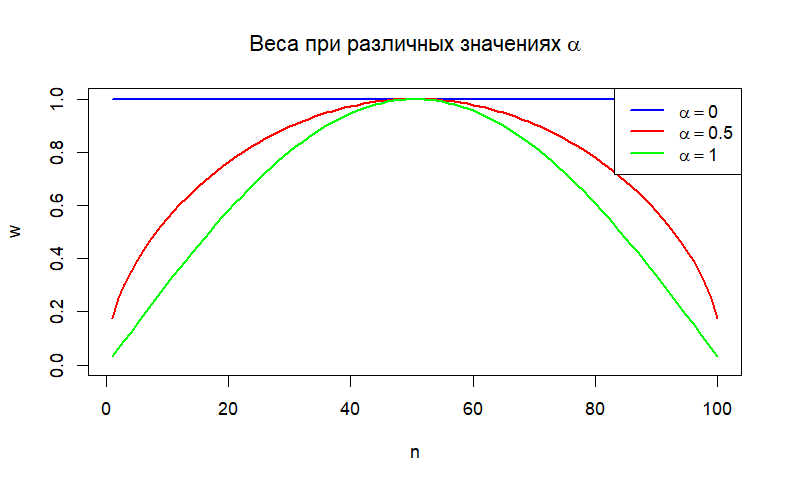
\includegraphics[width=0.8\textwidth]{img/weights.png} % Указываем путь к изображению и ширину
	\caption{График весов для различных значений \(\alpha\)} % Подпись под изображением
	\label{fig:weights} % Метка для ссылки на эту фигуру
\end{figure}


\subsubsection{Вложение}
$L$ --- некоторое целое число (длина окна), $1 < L < N$. Строится $L$-траекторная матрица $\mathbf{X}^{(\alpha)}$:
\begin{equation}
	\label{eq:X_alpha}
	\mathbf{X}^{(\alpha)} =
	\begin{pmatrix}
		w_1 x_1   & w_1 x_2     & w_1 x_3     & \dots  & w_1 x_{K}   \\
		w_2 x_2   & w_2 x_3     & w_2 x_4     & \dots  & w_2 x_{K+1} \\
		w_3 x_3   & w_3 x_4     & w_3 x_5     & \dots  & w_3 x_{K+2} \\
		\vdots    & \vdots      & \vdots      & \ddots & \vdots      \\
		w_L x_{L} & w_L x_{L+1} & w_L x_{L+2} & \dots  & w_L x_{N}
	\end{pmatrix}.
\end{equation}

\subsubsection{Сингулярное разложение (SVD)}
Этот шаг такой же, как и в $\SSA$, только матрица $\mathbf{X}$ заменяется на $\mathbf{X}^{(\alpha)}$. Будем обозначать собственные тройки в этом случае так: $(\sqrt{\lambda^{(\alpha)}},\,U^{(\alpha)},\,V^{(\alpha)})$.

\subsubsection{Группировка}
В точности как в $\SSA$. Тем самым, разложение может быть записано в сгруппированном виде:
\begin{equation*}
	\mathbf{X}^{(\alpha)} = \mathbf{X}^{(\alpha)}_{I_1} + \dots + \mathbf{X}^{(\alpha)}_{I_m}.
\end{equation*}

\subsubsection{Взвешенное диагональное усреднение}
Поскольку траекторная матрица была изменена весами, то диагональное усреднение тоже будет зависеть от весов.

Пусть $\mathbf{Y}$ --- матрица размерности $L \times K$. Взвешенное диагональное усреднение переводит матрицу $\mathbf{Y}$ в временной ряд $g_1, \dots, g_{N} $:

\begin{equation*}
	g_{k}=
	\begin{cases}
		\frac{1}{\sum_{n = 1}^k w_n} \sum\limits_{m=1}^{k+1} y_{m,k-m+2}^{*}           &
		\text{для } 1 \leq k < L,                                                        \\

		\frac{1}{\sum_{n = 1}^L w_n} \sum\limits_{m=1}^{L} y_{m,k-m+2}^{*}             &
		\text{для } L \leq k < K+1 ,                                                     \\

		\frac{1}{\sum_{n = k-K+1}^L w_n} \sum\limits_{m=k-K+2}^{N-K+1} y_{m,k-m+2}^{*} &
		\text{для } K+1 \leq k \leq N .                                                  \\
	\end{cases}
\end{equation*}
Применяя данную операцию к матрицам $\mathbf{X}_{I_1}^{(\alpha)}, \dots, \mathbf{X}_{I_m}^{(\alpha)}$, получаются $m$ новых рядов: $\TS^{(\alpha)}_1, \dots, \TS^{(\alpha)}_m$.
Результатом данного шага и всего алгоритма является разложение временного ряда $\TS^{(\alpha)}_1 + \dots + \TS^{(\alpha)}_m = \TS^{(\alpha)}$.



\subsection{Свойства GSSA}

\subsubsection{Веса}

Для минимизации эффекта спектрального размывания (spectral leakage), связанного с конечностью временного интервала наблюдений, к исходному ряду применялось оконное преобразование (tapering \cite{weisstein2002crc}). В качестве оконной функции используются степенные синус-косинусные веса (power-of-sine/cosine window).

Данное преобразование выполняет две ключевые функции:
\begin{enumerate}
	\item Снижение краевых эффектов: умножение исходного ряда на убывающую к краям функцию \( w(t) \);
	\item Сглаживание периодограммы: веса используются для усреднения значений.
\end{enumerate}

Такой подход позволяет более точно отделять компоненты ряда друг от друга.


\subsubsection{Ранг ряда}
Зафиксируем ряд $\TS = (x_1, \dots, x_{N})$ длины $N > 3$ и длину окна $L$.

%Рассмотрим базовый $\SSA$. В процессе процедуры вложения получаем последовательность векторов вложения:
%\begin{equation*}
%	\mathrm{X}_i^{(L)} = \mathrm{X}_i = (x_{i-1}, \dots, x_{i+L-2}), \quad i = 1, \dots, K,
%\end{equation*}
%$\mathcal{L}^{(L)} = \mathcal{L}^{(L)}(\TS) \stackrel{{\rm def}}{{=}} \operatorname{span}(\mathrm X_{1}, \ldots, \mathrm X_{K})$ --- траекторное пространство ряда $\TS$. 
%При этом, если $\dim \mathcal{L}^{(L)}= \operatorname{rank} \mathbf X = d$, то будем говорить, что ряд $\TS$ имеет $L$-ранг $d$ и записывать это как $\operatorname{rank}_L = d$.

В секции \ref{subsubsec: ssa_rank} было введено понятие ранга ряда для базового $\SSA$.
Теперь рассмотрим $\GSSA$ и поймем, что для того же ряда $\operatorname{rank} \mathbf{X}^{(\alpha)} = \operatorname{rank} \mathbf{X}$, а значит, что для $\GSSA$ также применимы понятия $L$-ранга ряда. Из вида \eqref{eq:X_alpha} $\mathbf{X}^{(\alpha)}$ можно получить, что $\mathbf{X}^{(\alpha)} = \operatorname{diag}\left(w_1, w_2, \dots, w_L \right) \mathbf{X} = \operatorname{diag}\left({\boldsymbol{w}}^{(a)}\right) \mathbf{X}$. Поскольку матрица $\operatorname{diag}\left({\boldsymbol{w}}^{(a)}\right)$ имеет ранг равный $L$, она диагональна, то и $\operatorname{rank} \mathbf{X}^{(\alpha)} = \operatorname{rank} \operatorname{diag}\left({\boldsymbol{w}}^{(a)}\right)\mathbf{X} = \operatorname{rank} \mathbf{X}$.

\subsubsection{GSSA как линейный фильтр}
Аналогично $\SSA$, метод $\GSSA$ можно переписать с помощью линейных фильтров.
Пусть $\TS = (x_1, \dots, x_{N})$ --- временной ряд длины $N$, $K = N - L + 1, \quad L^{*} = \min(L, K)$. Пусть $L$ будет длиной окна, а $(\sqrt{\lambda^{(\alpha)}},\,U^{(\alpha)},\,V^{(\alpha)})$ — одной из собственных троек. Определим диагональную матрицу $N \times N$:
$$
	\mathbf{D}^{(\alpha)} = \text{diag}(w_1, w_1 + w_2, \ldots,
	\sum \limits_{i = 1}^{L^*-1}w_i,
	\sum \limits_{i = 1}^{L^*}w_i, \sum \limits_{i = 1}^{L^*}w_i, \ldots, \sum \limits_{i = 1}^{L^*}w_i,
	\sum \limits_{i = 2}^{L^*}w_i, \ldots, w_{L^*-1}+ w_{L^*}, w_{L^*})
$$
и две матрицы  $K \times N$:
\[
	\mathbf{W}^{(\alpha)} = \begin{pmatrix}
		u_{1}^{(\alpha)} & u_{2}^{(\alpha)} & u_{3}^{(\alpha)} & \cdots           & u_{L}^{(\alpha)} & 0                & \cdots           & 0                & 0                & 0                \\
		0                & u_{1}^{(\alpha)} & u_{2}^{(\alpha)} & u_{3}^{(\alpha)} & \cdots           & u_{L}^{(\alpha)} & 0                & \cdots           & 0                & 0                \\
		\vdots           & 0                & \ddots           & \ddots           & \ddots           & \cdots           & \ddots           & 0                & \cdots           & 0                \\
		0                & \cdots           & 0                & u_{1}^{(\alpha)} & u_{2}^{(\alpha)} & u_{3}^{(\alpha)} & \cdots           & u_{L}^{(\alpha)} & 0                & \vdots           \\
		0                & 0                & \cdots           & 0                & u_{1}^{(\alpha)} & u_{2}^{(\alpha)} & u_{3}^{(\alpha)} & \cdots           & u_{L}^{(\alpha)} & 0                \\
		0                & 0                & 0                & \cdots           & 0                & u_{1}^{(\alpha)} & u_{2}^{(\alpha)} & u_{3}^{(\alpha)} & \cdots           & u_{L}^{(\alpha)}
	\end{pmatrix},
\]
\[
	\mathbf{W}_{\boldsymbol{w}}^{(\alpha)} = \begin{pmatrix}
		w_1 u_{1}^{(\alpha)} & w_2 u_{2}^{(\alpha)} & w_3 u_{3}^{(\alpha)} & \cdots               & w_L u_{L}^{(\alpha)} & 0                    & \cdots               & 0                    & 0                    & 0                    \\
		0                    & w_1 u_{1}^{(\alpha)} & w_2 u_{2}^{(\alpha)} & w_3 u_{3}^{(\alpha)} & \cdots               & w_L u_{L}^{(\alpha)} & 0                    & \cdots               & 0                    & 0                    \\
		\vdots               & 0                    & \ddots               & \ddots               & \ddots               & \cdots               & \ddots               & 0                    & \cdots               & 0                    \\
		0                    & \cdots               & 0                    & w_1 u_{1}^{(\alpha)} & w_2 u_{2}^{(\alpha)} & w_3 u_{3}^{(\alpha)} & \cdots               & w_L u_{L}^{(\alpha)} & 0                    & \vdots               \\
		0                    & 0                    & \cdots               & 0                    & w_1 u_{1}^{(\alpha)} & w_2 u_{2}^{(\alpha)} & w_3 u_{3}^{(\alpha)} & \cdots               & w_L u_{L}^{(\alpha)} & 0                    \\
		0                    & 0                    & 0                    & \cdots               & 0                    & w_1 u_{1}^{(\alpha)} & w_2 u_{2}^{(\alpha)} & w_3 u_{3}^{(\alpha)} & \cdots               & w_L u_{L}^{(\alpha)}
	\end{pmatrix}.
\]
Здесь $U = (u_1, \dots, u_L)$ --- собственный вектор матрицы $\mathbf{S}$.
\begin{theorem}
	\label{th:filter_GSSA}
	Компонента временного ряда $\widetilde \TS$, восстановленная с использованием собственной тройки $(\sqrt{\lambda^{(\alpha)}},\,U^{(\alpha)},\,V^{(\alpha)})$, имеет вид:
	\[
		\widetilde{\TS}^{{\rm T}} = {\mathbf{D}^{(\alpha)}}^{-1}
			{\mathbf{W}^{(\alpha)}}^{{\rm T}}
		\mathbf{W}_{\boldsymbol{w}}^{(\alpha)}
		\TS^{\rm T}.
	\]
\end{theorem}
\begin{proof}
	Доказательство проводится аналогично доказательству теоремы $\ref{th:filter_SSA}$.
\end{proof}

Таким образом, для восстановления методом $\GSSA$ средних точек (индексы от $L$ до $K$) имеем следующий фильтр:
\begin{equation}
	\label{eq:representation_gssa_as_filter}
	{\widetilde{x}}_{s} = \sum_{j=-(L-1)}^{L-1} \left( \sum_{k=1}^{L-|j|} u_{k}^{(\alpha)} u_{k+|j|}^{(\alpha)} w_k / \sum\limits_{i = 1}^{L}w_i \right) x_{s-j}, \quad L \leq s \leq K.
\end{equation}
Похожим образом можно переписать $\GSSA$ через линейные фильтры для точек в начале и конце.


\newpage




\section{Сравнение SSA и GSSA}
\label{sec:compare_ssa_gssa}
В данном разделе сравниваются алгоритмы базового $\SSA$ и $\GSSA$ с параметром $\alpha \not = 0$. Все вычисления, а также код метода $\GSSA$ можно найти в github репозитории \cite{spbu_cissa_coursework_github}.


\subsection{Линейные фильтры}
Чтобы понять их принципиальное отличие, рассмотрим методы с точки зрения линейных фильтров: по представлениям \eqref{eq:representation_ssa_as_filter} и \eqref{eq:representation_gssa_as_filter} можно построить амплитудно-частотные характеристики.

Рассмотрим временной ряд $\TS = \sin\left(\frac{2\pi}{12}x\right)$, $N = 96 \cdot 2 - 1$, $L = 48$.
Построим АЧХ для $\alpha$ равных $0$ (базовый $\SSA$), $\frac{1}{2}$, $1$, $2$:
\begin{figure}[H]
	\centering
	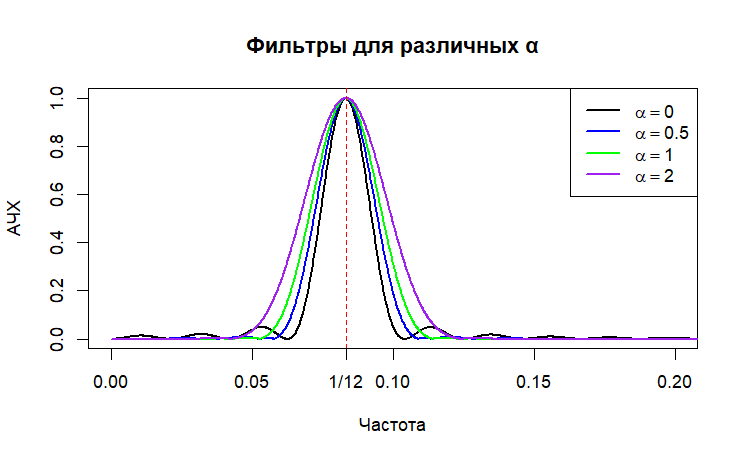
\includegraphics[width=1\textwidth]{img/various_alphas.png}
	\caption{АЧХ фильтров, отвечающих за $\TS = \sin\left(\frac{2\pi}{12}x\right)$, при разных $\alpha$}
	\label{fig:various_alphas}
\end{figure}
На рисунке \ref{fig:various_alphas} показано, как фильтры ведут себя для различных значений параметра \(\alpha\). Для всех рассмотренных значений \(\alpha\) фильтры подавляют частоты, значительно отличающиеся от частоты синуса $ \omega = \frac{1}{12}$. При малых значениях \(\alpha\), таких как \(\alpha = 0\), наблюдается волнообразное поведение фильтра, что указывает на частичное захватывание соседних частот, хотя и не близких к частоте синуса. С увеличением \(\alpha\) это волнообразное поведение уменьшается, и фильтр начинает захватывает больше частот, максимально близких к \(\frac{1}{12}\).

Таким образом, метод $\GSSA$ должен работать лучше $\SSA$ в случае, когда в временном ряде содержится пара периодических функций, частота одной из которых попадает в вершину волны АЧХ фильтра для другой функции. Например, добавим к $\TS_{\sin} = \sin\left(\frac{2\pi}{12} n \right)$ косинус с частотой $\frac{1}{19}$. Тогда $\TS = \TS_{\sin} + \TS_{\cos} = \sin\left(\frac{2\pi}{12} n \right) + \frac{1}{2}\cos\left(\frac{2\pi}{19} n \right)$, и можем рассмотреть АЧХ, отвечающие за синус, при базовом $\SSA$ ($\alpha = 0$) и $\GSSA$ при $\alpha = \frac{1}{2}$. При этом, $N = 96 \cdot 2 - 1$, $L = 48$.

\begin{figure}[H]
	\centering
	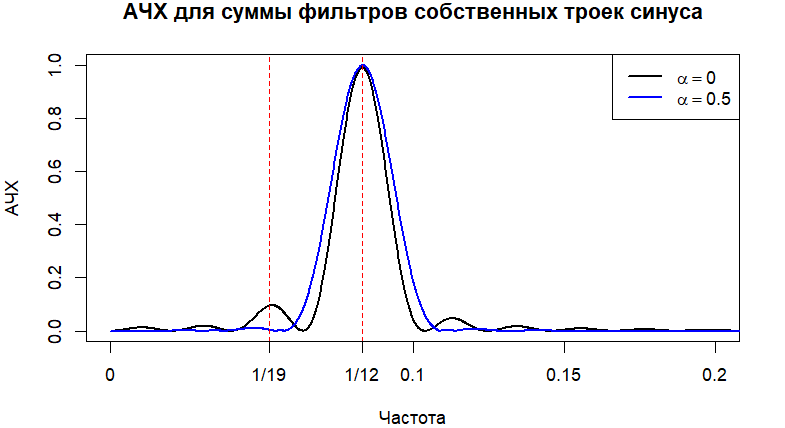
\includegraphics[width=1\textwidth]{img/various_alphas_sin_cos.png}
	\caption{Ряд $\TS = \TS_{\sin} + \TS_{\cos}$. АЧХ фильтров, отвечающих за $\TS_{\sin} = \sin\left(\frac{2\pi}{12} n \right)$, при разных $\alpha$}
	\label{fig:various_alphas_sin_cos}
\end{figure}

По рисунку \ref{fig:various_alphas_sin_cos} заметно, что фильтр для синуса в базовом $\SSA$ также частично захватит периодику с частотой $\frac{1}{19}$, в то время, как $\GSSA$ не будет испытывать таких проблем. Сравним результаты по среднеквадратичной ошибке:

\begin{table}[H]
	\caption{MSE разложений ряда $\TS = \TS_{\sin} + \TS_{\cos}$ для $\SSA$ и $\GSSA$ с $\alpha = \frac{1}{2}$}
	\centering
	\begin{tabular}{c|ccc}
		\hline
		Метод/Ошибка                  & $\TS_{\sin}$      & $\TS_{\cos}$      & $\TS$             \\
		\hline
		\textbf{SSA}                  & 5.15e-03          & 5.15e-03          & \textbf{6.01e-30} \\
		\textbf{GSSA}, $\alpha = 0.5$ & \textbf{3.68e-04} & \textbf{3.68e-04} & \textbf{9.53e-30} \\
		\hline
	\end{tabular}

	\label{tab:mse_ssa_gssa}
\end{table}

Как видно из таблицы \ref{tab:mse_ssa_gssa}, $\GSSA$ справился с разделением на порядок лучше $\SSA$.

Однако, у $\GSSA$ есть другая проблема. Если добавить к ряду шум, то оба алгоритма будут воспринимать этот шум как что-то близкое к частотам периодик, содержащихся в исходном ряде. А поскольку $\GSSA$ захватывает больше частот, максимально близких к периодикам, то и больше шума попадет в компоненты, отвечающие за периодики.

Добавим к $\TS$ шумовую компоненту: $\TS = \TS_{\sin} + \TS_{\cos} + \TS_{\mathrm{noise}} =
	\sin\left(\frac{2\pi}{12}x\right) +
	\frac{1}{2}\cos\left(\frac{2\pi}{19}x\right)+
	\varepsilon_n$,
где $\varepsilon_n \sim \mathrm N(0, 0.1^2)$, $N = 96 \cdot 2 - 1$, $L = 48$.
Проводилось $100$ тестов, в таблице \ref{tab:errs_ssa_gssa} указаны средние значения ошибки для одних и тех же реализаций шума.


\begin{table}[H]
	\caption{MSE разложений ряда $\TS = \TS_{\sin} + \TS_{\cos} + \TS_{\mathrm{noise}}$ для $\SSA$ и $\GSSA$ с $\alpha = \frac{1}{2}$}
	\label{tab:errs_ssa_gssa}
	\centering
	\begin{tabular}{c|ccc}
		\hline
		Метод                                 & $\TS_{\sin}$      & $\TS_{\cos}$      & $\TS$             \\
		\hline
		\textbf{SSA}                          & 5.68e-03          & 5.44e-03          & \textbf{7.48e-04} \\
		\textbf{GSSA}, $\alpha = \frac{1}{2}$ & \textbf{1.21e-03} & \textbf{1.25e-03} & 1.04e-03          \\
		\hline
	\end{tabular}

\end{table}

По таблице \ref{tab:errs_ssa_gssa} видно, что $\GSSA$ все же справился лучше $\SSA$, однако порядок ошибки теперь одинаковый для рассмотрения косинуса или синуса. Но при этом, отделение сигнала от шума получилось лучше у $\SSA$.
Также был проведен парный t-критерий для зависимых выборок с целью проверки гипотезы о равенстве средних значений ошибки для каждой компоненты. В качестве нулевой гипотезы ($H_0$) предполагалось, что средние значения двух сравниваемых выборок равны. Критический уровень значимости был установлен на уровне $\alpha_{\mathrm{hypothesis}} = 0.05$.
Результаты анализа показали, что во всех случаях $p$-значение оказалось меньше 0.05, что позволяет отвергнуть нулевую гипотезу.

\subsection{Отделение сигнала от шума}


Сингулярное разложение матрицы обладает наилучшими аппроксимационными свойствами в смысле минимизации нормы Фробениуса (или спектральной нормы) для заданного ранга. Из этого следует, что разложение матрицы $\mathbf{S} = \mathbf{X}\mathbf{X}^{\mathrm{T}}$ методом SVD будет наилучшим образом отделять сигнал от шума.

По результатам сравнений методов из таблиц \ref{tab:mse_ssa_gssa} и \ref{tab:errs_ssa_gssa}, а также предыдущих рассуждений, получается, что есть смысл использовать базовый $\SSA$ для выделения сигнала, а уже сам сигнал разделять на различные компоненты с помощью $\GSSA$.

Рассмотрим $\TS = \TS_{\sin} + \TS_{\cos} + \TS_{\mathrm{noise}} =
	\sin\left(\frac{2\pi}{12}x\right) +
	\frac{1}{2}\cos\left(\frac{2\pi}{19}x\right)+
	\varepsilon_n$,
где $\varepsilon_n \sim \mathrm N(0, 0.1^2)$, только теперь сначала применим $\SSA$, а затем $\GSSA$.
$N = 96 \cdot 2 - 1$, $L = 48$ для обоих методов.

\begin{table}[H]
	\centering
	\caption{$\TS_{\sin} + \TS_{\cos}+
			\varepsilon_n$, $\varepsilon_n \sim \mathrm N(0, 0.1^2)$, MSE оценок }
	\label{tab:errs_ssa_gssa_unite}
	\begin{tabular}{l|ccc}
		\hline
		Метод/Ошибка                     & $\TS_{\sin}$      & $\TS_{\cos}$      & $\TS$             \\
		\hline
		$\SSA$                           & 5.68e-03          & 5.44e-03          & \textbf{7.48e-04} \\
		$\GSSA$, $\alpha = 0.5$          & \textbf{1.21e-03} & \textbf{1.25e-03} & 1.04e-03          \\
		\hline
		$\SSA$ + $\GSSA$, $\alpha = 0.5$ & \textbf{1.06e-03} & \textbf{1.12e-03} & \textbf{7.15e-04} \\
		\hline
	\end{tabular}
\end{table}

Анализ данных, представленных в таблице \ref{tab:errs_ssa_gssa_unite}, позволяет сделать вывод, что комбинирование алгоритмов привело к улучшению как в выделении полезного сигнала, так и в разделении компонент между собой. Полученные результаты демонстрируют более высокую точность по сравнению с данными, приведёнными в таблице \ref{tab:errs_ssa_gssa}.


Таким образом, по приведенным примерам можно сделать вывод, что $\GSSA$ позволяет улучшить разделимость периодических компонент ряда. Однако, вместе с тем, разложение будет захватывать больше шума в сравнении с базовым $\SSA$.


\subsection{Фильтры в различных точках}
В зависимости от точек ряда, линейные фильтры будут отличаться друг от друга. Рассмотрим тот же пример $\TS = \TS_{\sin} + \TS_{\cos} + \TS_{\mathrm{noise}} =
	\sin\left(\frac{2\pi}{12}x\right) +
	\frac{1}{2}\cos\left(\frac{2\pi}{19}x\right)+
	\varepsilon_n$,
где $\varepsilon_n \sim \mathrm N(0, 0.1^2)$.
\begin{figure}[H]
	\centering
	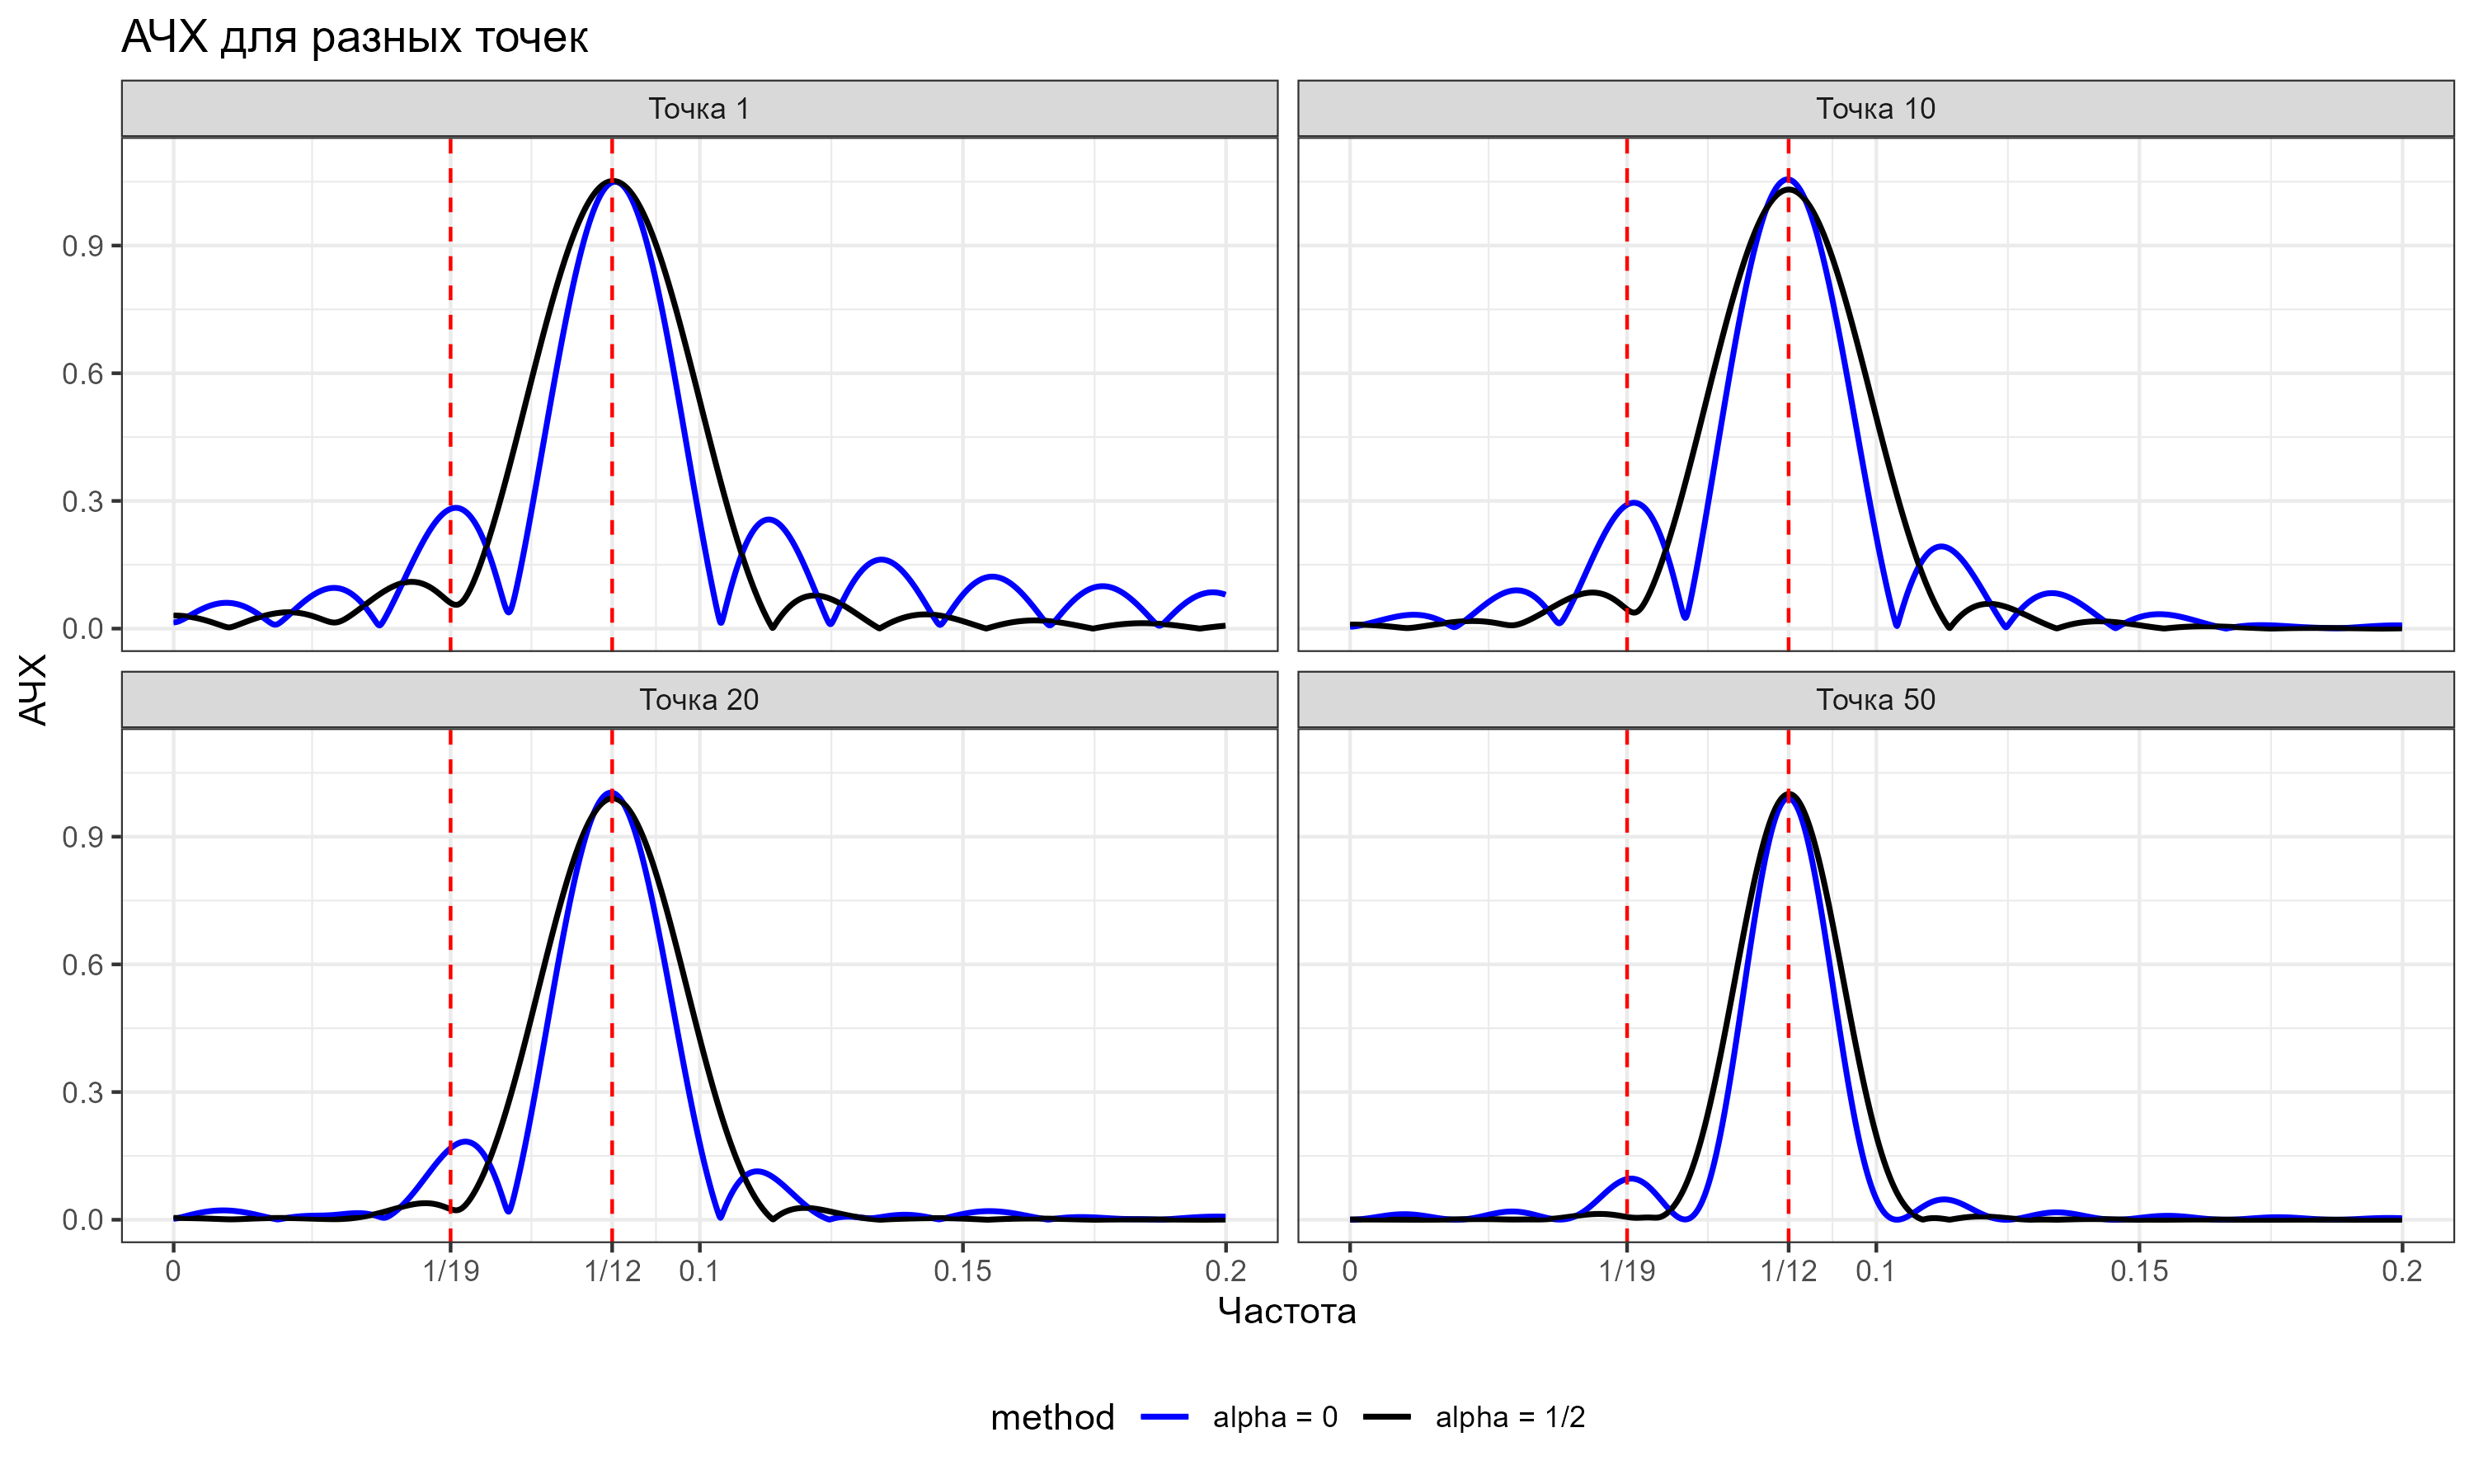
\includegraphics[width=1\textwidth]{img/afc_4_points.png}
	\caption{Ряд $\TS = \TS_{\sin} + \TS_{\cos}+ \TS_{\mathrm{noise}}$. АЧХ фильтров в разных точках, отвечающих за $\TS_{\sin} = \sin\left(\frac{2\pi}{12} n \right)$, при разных $\alpha$}
	\label{fig:filter_point_depends}
\end{figure}

По рисунку \ref{fig:filter_point_depends} видно, что когда точка s приближается по времени к средним точкам временного ряда ($L \leq s \leq K$), полоса пропускания фильтра становится уже, а также фильтр начинает все меньше и меньше захватывать соседние частоты.

Для этого примера также можно посмотреть на график средней MSE ошибки в зависимости от точки ряда. Эксперимент проводился 1000 раз.
\begin{figure}[H]
	\centering
	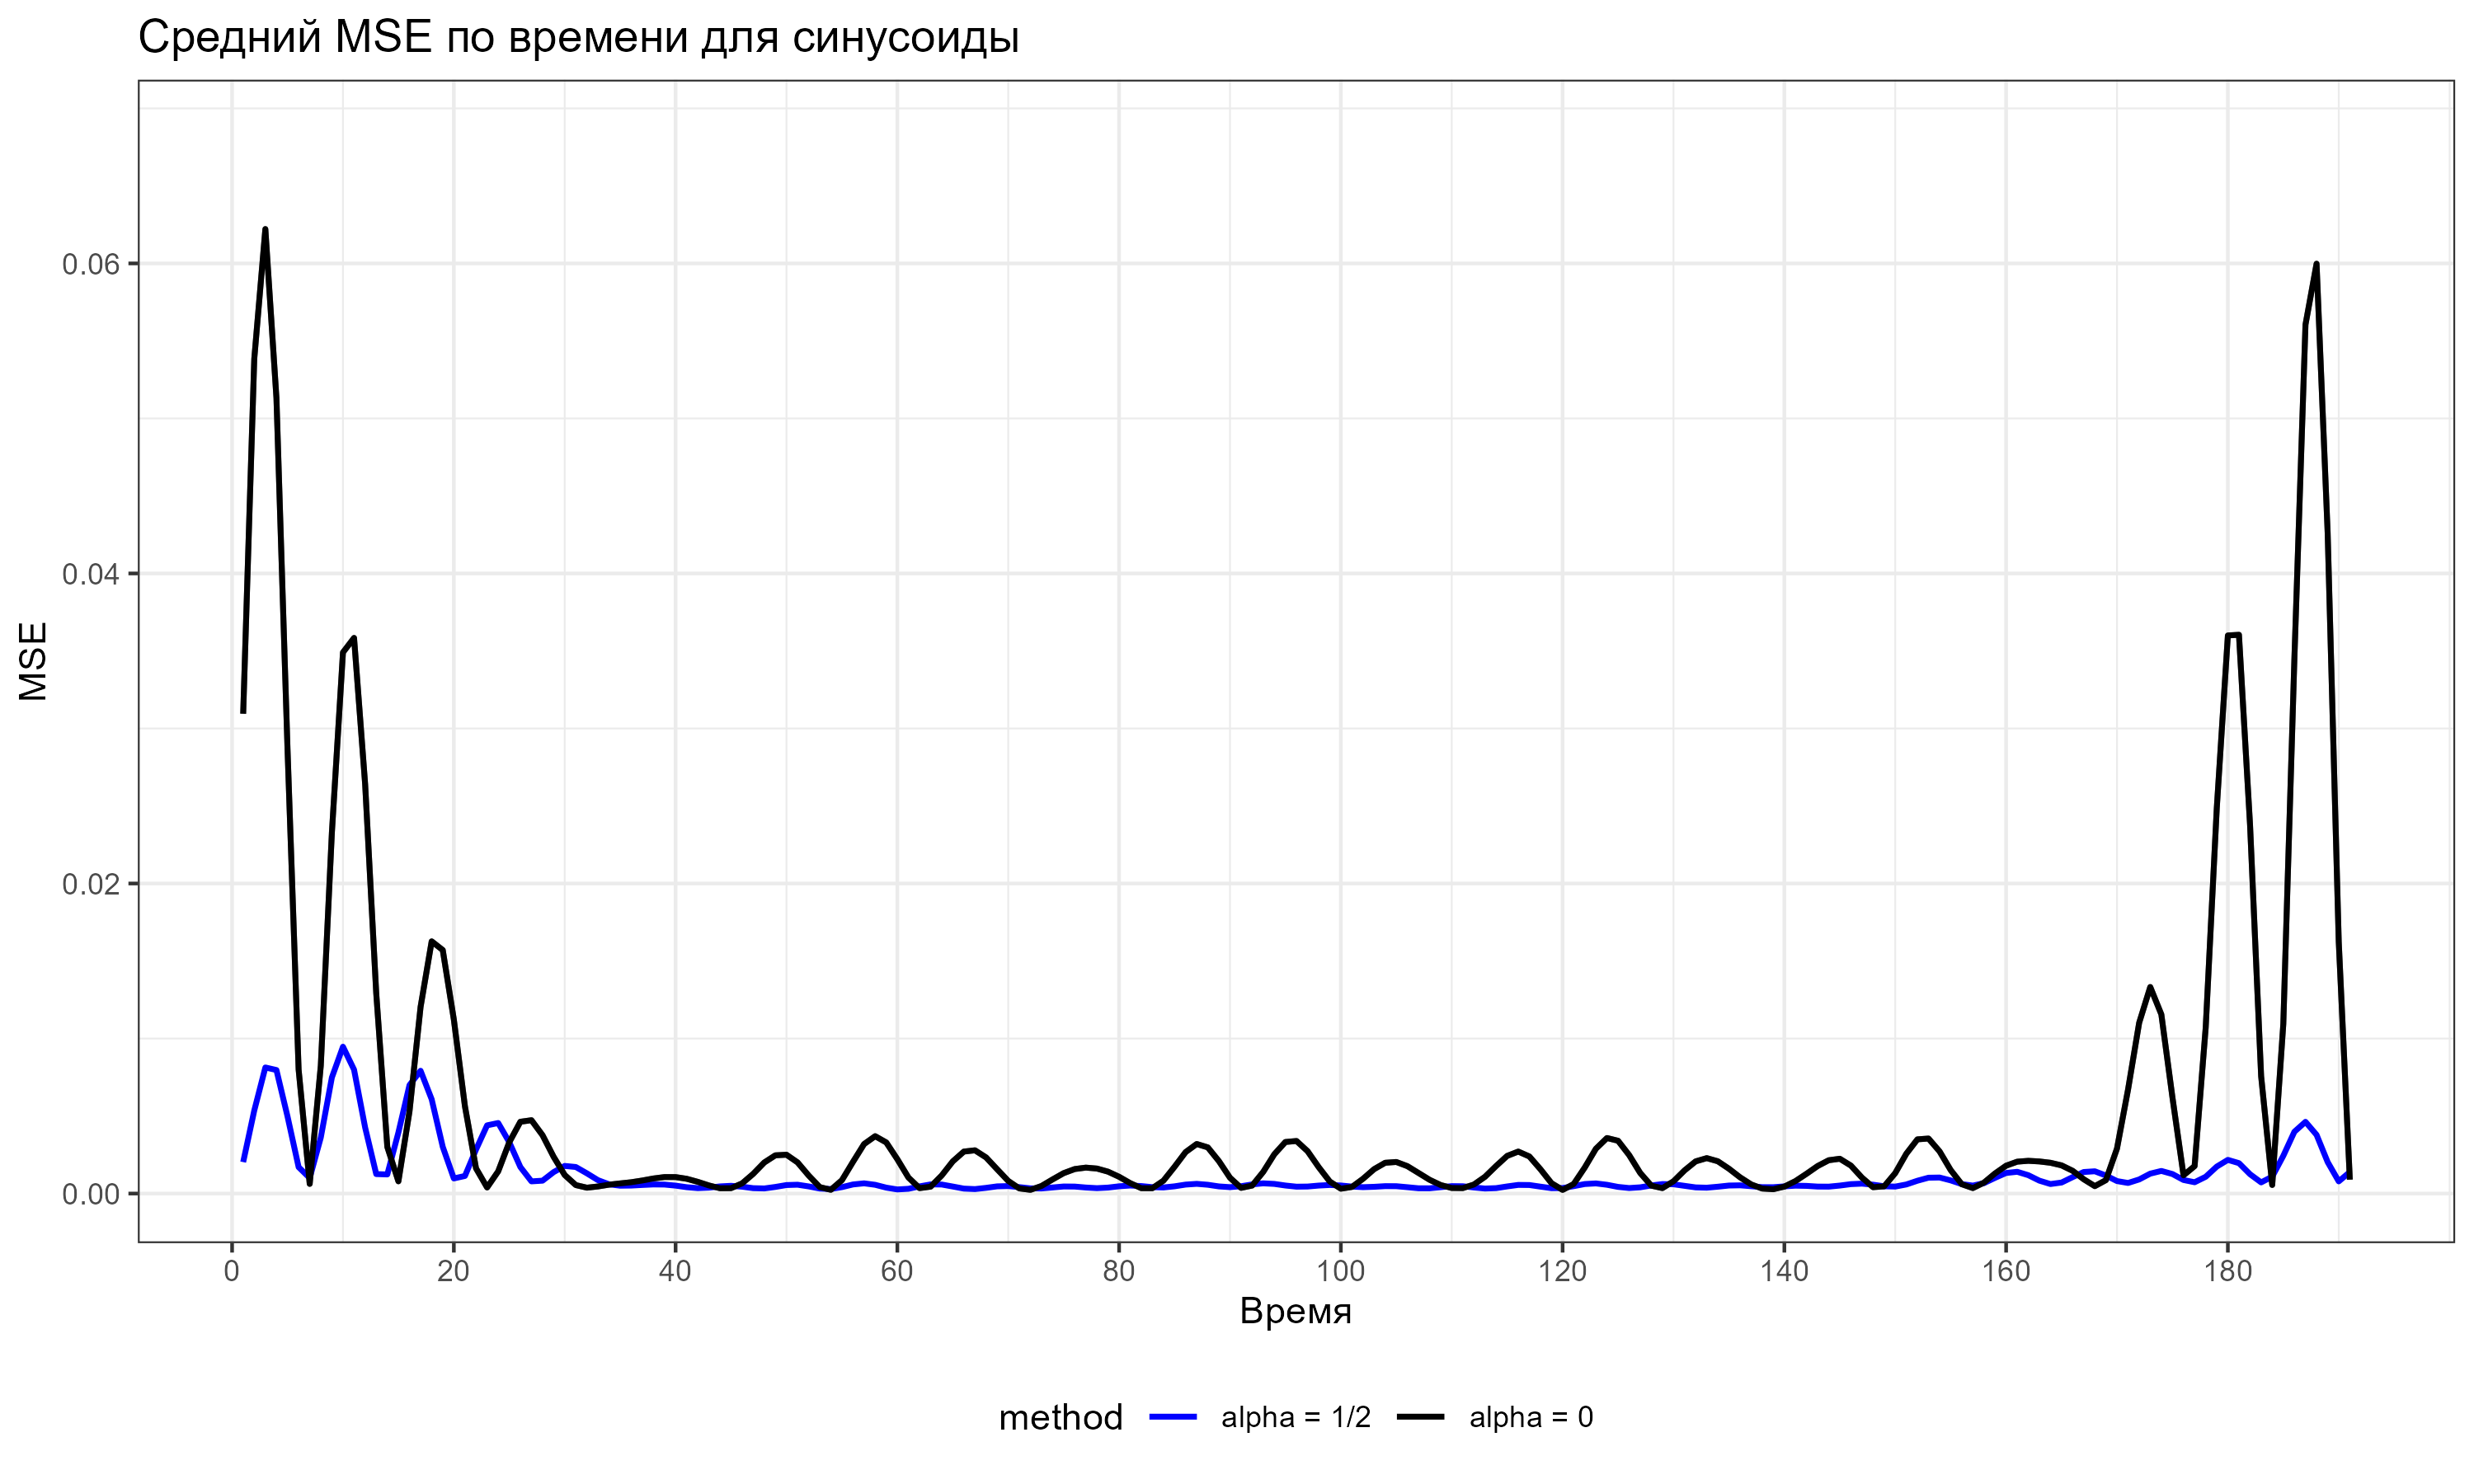
\includegraphics[width=1\textwidth]{img/mse_y1_time.png}
	\caption{Ряд $\TS = \TS_{\sin} + \TS_{\cos}+ \TS_{\mathrm{noise}}$. MSE ошибки выделения синуса в зависимости от точки ряда}
	\label{fig:mse_filter_point_depends}
\end{figure}

Таким образом, можно сделать вывод, что разделимость также зависит от точки ряда. В средних точках достигаются наилучшие значения ошибки. Однако это не означает, что нужно брать маленькое $L$, поскольку чем больше длина окна, тем лучше происходит разделение компонент между собой в целом \cite{golyandina2001analysis}.


\newpage






\section{Метод Circulant singular spectrum analysis (CiSSA)}
\label{sec:cissa}

%* Переформулировка начала секции 3 из статьи про $\CISSA$ от третьего лица (сказать зачем он создавался, т.е. для автоматического выделения частот)

В этом разделе описана модификация $\SSA$ на основе циркулярной матрицы \cite{bogalo2020}. В отличие от базового $\SSA$, в $\CISSA$ для каждого конкретного $L$ базис разложения остается одинаковым для любого входного временного ряда. Поскольку из-за этого повышается интерпретируемость каждой компоненты в разложении, авторы метода назвали $\CISSA$ автоматизированной версией $\SSA$. Причем автоматизированная в том смысле, что компоненты ряда группируются по частотам самим алгоритмом. Сначала будет рассмотрен метод только для стационарного случая, затем показана применимость модифицированной версии $\CISSA$ при использовании нестационарного ряда.

Стационарность подразумевает неизменность статистических свойств ряда во времени. Определим это понятие формально \cite{golyandina2001analysis}.
\begin{definition}
	Пусть $\TS = (x_1, \dots, x_n, \dots)$ — временной ряд. Ряд $\TS$ называется стационарным, если существует функция $R_{\TS}(k)$ ($-\infty < k < +\infty$) такая, что для любых $k, l \geq 1$
	\begin{equation}
		R_{\TS}^{(N)}(k, l) \overset{\mathrm{def}}{=} \frac{1}{N} \sum_{m=1}^{N} x_{k+m} x_{l+m} \xrightarrow{N \to \infty} R_{\TS}(k - l). \label{eq:R}
	\end{equation}

	Если \eqref{eq:R} выполняется, тогда $R_{\TS}$ называется ковариационной функцией стационарного ряда $\TS$.
\end{definition}

\begin{theorem}
	Пусть $R_{\TS}$ — ковариационная функция стационарного ряда $\TS$. Тогда существует конечная мера $m_{\TS}$, определенная на борелевских подмножествах $(-1/2, 1/2]$, такая, что
	\[
		R_{\TS}(k) = \int_{(-\frac{1}{2}, \frac{1}{2}]} e^{i 2 \pi k \omega} m_{\TS}(d\omega).
	\]


	Мера $m_{\TS}$ называется спектральной мерой ряда $\TS$.
\end{theorem}
\begin{proof}
	Доказательство в \cite{golyandina2001analysis}.
\end{proof}

%\begin{definition}
%	 ряд $\TS = (x_1, x_2, x_3, \dots)$ называется стационарным, если:
%	\begin{enumerate}
%		\item $\mathrm E (x_t) \equiv \mathrm{const}, \, \forall t \in 1:N$;
%		\item $\mathrm{Cov}(x_t, x_{t+h}) \equiv \mathrm{const}$ при фиксированном h.
%	\end{enumerate}
%\end{definition}

\subsection{Алгоритм метода CiSSA}
%План:
%\begin{enumerate}
%	\item Алгоритм в текстовом виде.
%	\item ??? Алгоритм на псевдокоде.
%	\item Кратко указать, почему он работает (сослаться на доказательства в статье)
%	\item Пояснить, что делать с нестационарными рядами, показать расширение ряда
%	\item Кратко упомянуть, что алгоритм был реализован на языке R, сослаться на код в GitHub.
%\end{enumerate}

Данный алгоритм, как и $\SSA$, состоит из четырех основных шагов.

Зафиксируем стационарный временной ряд $\TS$ состоящий из $N$ элементов и выберем длину окна $L$.
\subsubsection{Вложение}
Такой же, как и в $\SSA$. Считаем матрицу $\mathbf{X}$, заданную в \eqref{eq:X}.

\subsubsection{Разложение}

Для каждого $k = 1:L$ вычисляются собственные векторы ${U}_{k}$:
\begin{equation*}
	{U}_{k}=L^{-1/2}(u_{k,1\cdot}\cdot\cdot\cdot,u_{k,L}), \, \text{где} \,
	u_{k,j}=\exp\left(-\mathrm{i}2\pi(j-1)\frac{k-1}{L}\right), \,
	\text{причем} \, U_{k} = U_{L+2-k}^*,
\end{equation*}
где $U^*$ --- комплексное сопряжение вектора $U$.


\paragraph{Элементарное разложение \newline}

Для каждой частоты $w_k = \frac{k-1}{L}$, $k = 1:\lfloor \frac{L+1}{2} \rfloor$, есть два собственных вектора: $U_k$ и $U_{L+2-k}$. За частоту $w_0$ отвечает один собственный вектор --- $U_0$. Если же $L$ --- четное, то частоте $w_{\frac{L}{2} + 1}$ будет соответствовать один вектор $U_{\frac{L}{2}+1}$.

Следовательно, индексы группируются следующим образом:
\begin{equation*}
	B_1 = \{1\}; \, B_k = \{k, L+2-k\}, \,  \text{для } k = 1:\lfloor \frac{L+1}{2}\rfloor; \,
	B_{\frac{L}{2} + 1} = \left\{ \frac{L}{2} + 1 \right\}, \, \text{если} \, L\mod 2 = 0.
\end{equation*}
%Разложение $\mathbf X_{B_k} = \mathbf X_k + \mathbf X_{L+2-k} = U_k U_k^H \mathbf X + U_{L+2-k} U_{L+2-k}^H \mathbf X$, где $U^H$ --- это комплексное сопряжение и транспонирование вектора $U$.

Таким образом, получается элементарная группировка по частотам $w_k$:
\begin{align*}
	\mathbf X_{B_k}                 & = \mathbf X_k + \mathbf X_{L+2-k} = U_k U_k^H \mathbf X + U_{L+2-k} U_{L+2-k}^H \mathbf X, \,  \text{для } k = 1:\lfloor \frac{L+1}{2}\rfloor; \\
	\mathbf X_{B_{\frac{L}{2} + 1}} & = \mathbf X_{{\frac{L}{2} + 1}} =
	U_{\frac{L}{2} + 1} U_{\frac{L}{2} + 1}^H \mathbf X, \, \text{если} \, L \mod 2 = 0,
\end{align*}
где $U^H$ --- это комплексное сопряжение и транспонирование вектора $U$.

Пусть $d = \lfloor \frac{L+1}{2} \rfloor$, если $L \mod 2 \not = 0$, иначе $d = \frac{L}{2} + 1$. Тогда результатом данного шага будет разложение исходной матрицы $\mathbf X$ в сумму матриц $\mathbf{X}_{B_k}$, отвечающих периодикам с определенными частотами $w_k$:
\begin{equation*}
	\mathbf X = \sum\limits_{k=1}^d \mathbf{X}_{B_k} .
\end{equation*}


\subsubsection{Группировка}
Такой же шаг, как и в базовом $\SSA$. Однако группировка будет производиться на непересекающиеся подгруппы по частотам от $w_k$, которые находятся в диапазоне от $0$ до $0.5$. То есть, заранее заданному произвольному количеству непересекающихся диапазонов $I_i = \left[w_{\mathrm{i0}}, w_{\mathrm{i1}}\right]$, $w_{\mathrm{i0}} \leq w_{\mathrm{i1}}$ и $0 \leq w_{\mathrm{i0}}, w_{\mathrm{i1}} \leq 0.5$, строятся матрицы $\mathbf X_{I_i}$, в которые входят суммы $\mathbf X_{B_k}$, отвечающие частотам $w_k: w_{i0} \leq w_k \leq w_{i1}$.

\subsubsection{Диагональное усреднение}
Такой же шаг, как и в базовом $\SSA$.

\begin{comment}
$U_k$ можно получить по аналогии с $\SSA$.

Будем рассматривать временной ряд как выборку после эксперимента, а не как случайную величину. Соответственно, все формулы будут выборочными.

Определим автоковариации:
\begin{equation*}
	\hat{\gamma}_m = \frac{1}{N-m} \sum \limits_{t = 1}^{N-m}x_t x_{t+m}, \, m = 0:(L-1).
\end{equation*}
На основе $\hat{\gamma}_m$ определим матрицу:
\begin{equation}
	\label{eq:tepl_mat}
	\hat{\gamma}_{L}=\left(\begin{array}{cccc}
			\hat{\gamma}_{1} & \hat{\gamma}_{2}   & \ldots & \hat{\gamma}_{L}   \\
			\hat{\gamma}_{2} & \hat{\gamma}_{1}   & \ldots & \hat{\gamma}_{L-1} \\
			\vdots           & \vdots             & \vdots & \vdots             \\
			\hat{\gamma}_{L} & \hat{\gamma}_{L-1} & \hdots & \hat{\gamma}_{1}
		\end{array}\right).
\end{equation}
Данная матрица $L \times L$ называется Теплицевой и используется в методе Toeplitz SSA (подробнее про данный метод можно прочитать в книге \cite{golyandina2001analysis}). На ее основе составим циркулярную матрицу для алгоритма Circulant SSA \cite{bogalo2020}:


\begin{equation}
	\label{eq:circ_mat}
	\hat{\mathrm{C}}_{L}=\left(\begin{array}{cccc}
			\hat c_{1} & \hat c_{2}   & \ldots & \hat c_{L}   \\
			\hat c_{2} & \hat c_{1}   & \ldots & \hat c_{L-1} \\
			\vdots     & \vdots       & \vdots & \vdots       \\
			\hat c_{L} & \hat c_{L-1} & \hdots & \hat c_{1}
		\end{array}\right),
\end{equation}
где $\hat c_m = \frac{L-m}{L}\hat{\gamma}_m + \frac{m}{L}\hat{\gamma}_{L-m}, \, m = 0:L-1$.
Собственные числа матрицы $\hat{\mathrm{C}}_{L}$, определенной в \eqref{eq:circ_mat} задаются по формуле:
\begin{equation*}
	\lambda_{L,k}=\sum_{m=0}^{L-1}\hat c_{m}\exp\left(i 2\pi m\frac{k-1}{L}\right), \, k = 1:L, \, \text{причем} \, \lambda_{L,k} = \lambda_{L,L+2-k},
\end{equation*}
а собственные вектора, связанные с $\lambda_{L, k}$ --- это векторы $U_k$.
\end{comment}

\begin{comment}
\label{comm:proector}
$U_k U_k^H + U_{L+2-k} U_{L+2-k}^H$ является оператором проектирования на подпространство, которое порождено синусами и косинусами с частотой $w_k = \frac{k-1}{L}$. Это пространство соответствует компонентам синусоидальной структуры временного ряда, связанных с конкретной частотой, выделяемой методом.
\end{comment}
\begin{proof}
	Рассмотрим на примере одного вектора-столбца $X_i = \left(x_i, \dots, x_{i+L}\right)^{\mathrm T}$, где $i = 1, \dots, K$. Возьмем для наглядности $i = 1$.
	$$
		U_k = L^{-\frac{1}{2}}\left(1, e^{-i2\pi \frac{k-1}{L}}, e^{-i2\pi 2\frac{k-1}{L}}, \dots, e^{-i2\pi (L-1)\frac{k-1}{L}}\right)^{\mathrm T},
	$$
	$$
		U_k^H = L^{\frac{1}{2}}\left(1, e^{i2\pi \frac{k-1}{L}}, e^{i2\pi 2\frac{k-1}{L}}, \dots, e^{i2\pi (L-1)\frac{k-1}{L}}\right).
	$$
	$$
		L^{-\frac{1}{2}}c_k = U_k^H X_1 = x_1 + e^{i2\pi \frac{k-1}{L}} x_2 + e^{i2\pi 2\frac{k-1}{L}} x_3 + \dots + e^{i2\pi (L-1)\frac{k-1}{L}} x_L.
	$$
	$$
		X_1^k = c_k U_k = \left(c_k, c_k e^{-i2\pi \frac{k-1}{L}}, c_k e^{-i2\pi 2\frac{k-1}{L}}, \dots, c_k e^{-i2\pi (L-1)\frac{k-1}{L}}\right)^{\mathrm T}.
	$$
	Таким образом, получилось проектирование на пространство синусов и косинусов, если разложить комплексную экспоненту.
	Если брать всю матрицу $\mathbf X$, выйдет $K$ столбцов, спроектированных на данное пространство.
\end{proof}
\begin{comment}
В разделе \ref{subsec:cissa_fourier} рассмотрена связь между матрицей $\mathbf X_{B_k}$ и разложениями Фурье для векторов вложения.
\end{comment}

\noindent \textbf{\large{Нестационарный случай}} \newline \newline
Для применения данного алгоритма на нестационарных временных рядах, нужно применить процедуру расширения ряда. Как утверждается авторами статьи \cite{bogalo2020}, после расширения, $\CISSA$ можно применить к нестационарному ряду.
Сама процедура расширения ряда $\TS$ производится с использованием авторегрессионной (AR) модели. Эта процедура позволяет предсказать значения временного ряда за его пределами (экстраполяция) как в правом, так и в левом направлениях на заданное число шагов $H$. Таким образом, трендовая (нелинейная) компонента ряда будет выделяться заметно лучше. В ходе работы алгоритм выполняет следующие шаги:
\begin{enumerate}
	\item \textbf{Определение порядка AR-модели}:
	      Метод определяет порядок $p$ AR-модели как целую часть от деления длины ряда $N$ на 3. Это значение порядка модели $p$ будет использовано для построения авторегрессионной модели на дифференцированном временном ряде;

	\item \textbf{Построение дифференцированного ряда}:
	      Временной ряд $\TS$ сначала преобразуется в дифференцированный ряд $d \TS$, чтобы удалить трендовые компоненты;

	\item \textbf{Построение AR-модели}:
	      После этого для дифференцированного ряда вычисляются коэффициенты авторегрессионной модели $A$ с использованием метода Юла-Уокера, основываясь на определенном ранее порядке $p$;

	\item \textbf{Правое расширение ряда}:
	      С помощью AR-модели ряд $d\TS$ прогнозируется на $H$ шагов вправо. Затем возвращается к своему изначальному состоянию путем интегрирования $d\TS$. Получается расширение исходного ряда $\TS$ на $H$ шагов вправо;

	\item \textbf{Левое расширение ряда}:
	      Аналогично предыдущему пункту, ряд прогнозируется на $H$ шагов влево;

	\item \textbf{Возвращение расширенного ряда}:
	      В конце метод возвращает расширенный временной ряд $\TS_{\mathrm{extended}}$, который содержит как левое, так и правое расширение на $H$ шагов от исходного ряда $\TS$.
\end{enumerate}


Таким образом, алгоритм расширения ряда позволяет выполнять предсказания временного ряда по обе стороны от его границ, основываясь на авторегрессионной модели, построенной на дифференцированном ряде, что полезно для выделения тренда.
\begin{figure}[H]
	\centering
	\includegraphics[width=1\textwidth]{img/extended_IP_values.png}
	\caption{Расширение временного ряда IP values. Красным показан настоящий ряд, черным --- его расширение}
	\label{fig:extended_IP_values}
\end{figure}
Однако поскольку мы рассматриваем расширенный ряд, то и периодические компоненты будут строиться по нему. Поэтому в угоду лучшего выделения трендовой составляющей, будет несколько жертвоваться точность разделения периодических компонентов.
\begin{figure}[H]
	\centering
	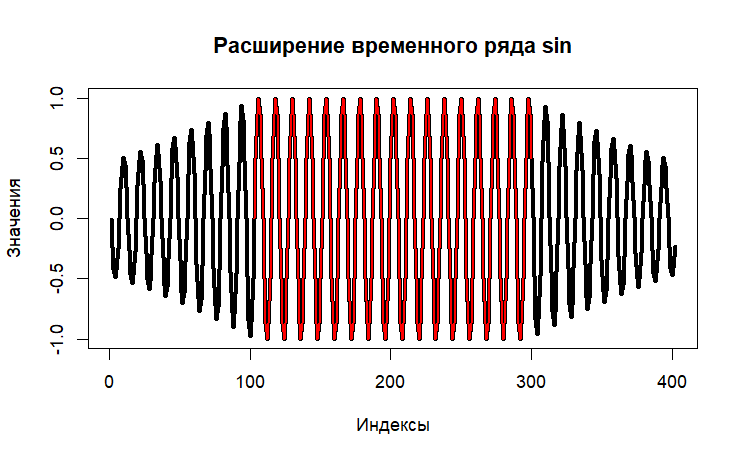
\includegraphics[width=1\textwidth]{img/extended_sin.png}
	\caption{Расширение временного ряда синуса. Красным показан настоящий ряд, черным --- его расширение}
	\label{fig:extended_sin}
\end{figure}

На рисунке \ref{fig:extended_sin} видно, что синус расширился неправильно, от концов настоящего ряда до концов расширенного значения постепенно уменьшались. Как будет показано в секции \ref{sec:comparison_cissa}, это повлияет на значения ошибки.




\subsection{Свойства}

%\subsubsection{Асимптотическая эквивалентность методов}
%В статье \cite{bogalo2020} говорится, что асимптотически методы $\SSA$ и $\CISSA$ эквивалентны в случае стационарного ряда и в доказательство приводится теорема \ref{th:equiv}.
%
%\begin{definition}
%	Будем говорить, что методы $M_1$ и $M_2$ асимптотически эквивалентны, если их матрицы вложения $S_1$, $S_2$ асимптотически эквиваленты в смысле $\operatorname*{lim}\limits_{L\rightarrow\infty \, N\rightarrow\infty}\frac{\|{S_1-S_2}\|_F}{\sqrt{L}}=0$, при некоторой последовательности $L = L(N) $, $N \rightarrow \infty$, где $\|{\cdot}\|_F$ --- норма Фробениуса. Тогда $M_1 \sim M_2$, $S_1 \sim S_2$.
%\end{definition}
%
%\begin{theorem}
%	\label{th:equiv}
%	Пусть $\TS$ --- стационарный временной ряд.
%	Дана $L \times K$ траекторная матрица $\mathbf{X}$, определенная в \eqref{eq:X}. Пусть $S_B = \mathbf{X} \mathbf{X}^T / K$, $S_T$ --- матрица, определенная в \eqref{eq:tepl_mat}, $S_C$ --- матрица, определенная в \eqref{eq:circ_mat}. Тогда $S_B \sim S_T \sim S_C$.
%\end{theorem}
%
%\begin{proof}
%	Доказательство в источнике \cite{bogalo2020}.
%\end{proof}
%
%
%Теорема \ref{th:equiv} дает понимание похожих практических результатов при применении разных методов.

\subsubsection{Связь CiSSA с разложением Фурье}
\label{subsec:cissa_fourier}
Для описания конечных, но достаточно длинных рядов можно использовать разложение Фурье. Пусть $\TS = (x_1, \dots, x_N)$ — временной ряд
\begin{definition}
	Разложение
	\begin{equation}
		\label{eq:fourier}
		x_n = c_0 + \sum\limits_{k = 1}^{\lfloor \frac{N+1}{2} \rfloor}\left(c_k \cos(2\pi n k / N) + s_k \sin(2\pi n k / N) \right),
	\end{equation}
	где $1 \leq n \leq N$ и $s_{N/2} = 0 $ для четного N, называется разложением Фурье ряда $\TS$.
\end{definition}

Таким образом, можно выделить компоненту ряда, отвечающую за частоту $w_k = \frac{k-1}{L}$, $k = 1:\lfloor \frac{N+1}{2} \rfloor$;

Алгоритм $\CISSA$ тесно связан с разложением Фурье. По замечанию \ref{comm:proector} видно, что при вычислении $\mathbf X_{B_k} = \mathbf X_k + \mathbf X_{L+2-k} = U_k U_k^H \mathbf X + U_{L+2-k} U_{L+2-k}^H \mathbf X$, воспроизводится разложение Фурье для $K$ векторов матрицы $\mathrm X$. Затем вычисляется диагональное усреднение $\mathbf X_{B_k}$. А именно, $\CISSA$ можно представить так:
\begin{enumerate}
	\item Вычисляем разложение Фурье для каждого вектора вложения $L$-траекторной матрицы $\mathbf{X}$, состоящей из $K = N - L + 1$ векторов. Получается $K$ разложений Фурье по частотам $w_k = \frac{k-1}{L}$, $k = 1:\lfloor \frac{L+1}{2} \rfloor$;
	\item По получившимся разложениям Фурье усредняем значения для соответствующих $x_i$ и частот $w_k$.
\end{enumerate}

\subsubsection{Точная разделимость}
Поскольку данный метод является аналогом разложения Фурье, то в смысле сильной разделимости можно точно разделить ряд, в котором одной из компонентов является $\cos(2\pi \omega + \varphi)$ с частотой $\omega$ такой, что $L\omega = k \in \mathbb N$, или константа. Для сравнения, при применении базового $\SSA$, условие накладывалось не только на $L\omega \in \mathbb N$, но и на $K\omega \in \mathbb N$.

Поэтому до применения алгоритма необходимо выделить интересующие частоты, то есть знать их заранее, и, исходя из них, выбирать значение $L$.

\subsubsection{Асимптотическая разделимость}
Асимптотическая разделимость в данном случае будет означать, что при увеличении $L$ разбиение сетки будет увеличиваться, а значит, и частоты в сетке начнут сближаться к истинным частотам периодических компонентов (либо становиться равными им), что будет снижать ошибку вычислений.

То есть, в случае непопадания периода определенной компоненты в разбиение частот алгоритма, будет выполняться $\CISSA$-асимптотическая $L(N)$-разделимость по определению \ref{def:asymp}.


\subsection{Обзор литературы}

% ? Лучше не делать отдельной секцией ? 

В данной секции рассмотрены применения $\CISSA$ на практике.

\subsubsection{Cognitive Load Detection through EEG Lead-Wise Feature Optimization and Ensemble Classification}

В статье~\cite{cognitive} рассматриваются несколько наборов данных ЭЭГ под различной нагрузкой, два из которых наиболее значимы:

\begin{itemize}
	\item \textbf{MAT (Mental Arithmetic Task)}: участие студентов в задаче на математический счёт.
	\item \textbf{STEW (Simultaneous Task EEG Workload)}: параллельное выполнение нескольких заданий.
\end{itemize}

Задача исследования заключалась в следующем:

\begin{itemize}
	\item С помощью метода $\CISSA$ (и других различных методов) разлагают исходные сигналы ЭЭГ на несколько компонент, каждая из которых несёт информацию о разных частотных диапазонах и временных структурах.
	\item После разложения из полученных компонент (или их комбинаций) вычисляют числовые признаки: энергетические, энтропийные и другие.
	\item Эти признаки затем подают на вход классификатору (например, $k$NN, SVM или другому алгоритму машинного обучения), чтобы автоматически определить уровень когнитивной нагрузки. Классификация может быть как бинарной (наличие/отсутствие нагрузки), так и многоуровневой (лёгкая/средняя/высокая нагрузка).
\end{itemize}

Таким образом, метод CiSSA был выбран в качестве одного из подходов разложения сигнала по частотам.

Выводом исследования является таблица 5 статьи~\cite{cognitive}, в которой авторы сравнивают по метрикам различные решения задачи. Подходы, связанные с $\CISSA$, являются не самыми наилучшими.



\subsubsection{Application of visual stratigraphy from line-scan images to constrain chronology and melt features of a firn core from coastal Antarctica}

В работе \cite{Dey_Thamban_Laluraj_Mahalinganathan_Redkar_Kumar_Matsuoka_2023} исследовалось таяние ледников, а также анализировались данные визуальной стратиграфии (VS) для построения хронологии фирнового керна из прибрежной Антарктиды. Основной задачей было отделение долгосрочного тренда, связанного с изменением плотности фирна, от сезонных сигналов, обусловленных включениями пыли и морской соли.
Для разложения сигнала по частотам был выбран алгоритм $\CISSA$. Длина окна была установлена равной 10, поскольку "дальнейшее её увеличение не оказывало существенного влияния на результаты".

\noindent \textbf{Ключевые этапы анализа}

\begin{itemize}
	\item \textbf{Первая компонента (RC1)}: отвечала за долгосрочный тренд, связанный с постепенным увеличением плотности фирна с глубиной;
	\item \textbf{Компоненты со второй по пятую (RC2-RC5)}: отражали сезонность, обусловленную изменениями в содержании пыли и морских солей;
	\item \textbf{Остальные компоненты}: содержали шумовой сигнал и не учитывались в дальнейшем анализе.
\end{itemize}

Таким образом, метод CiSSA был использован как инструмент частотного разложения.

\subsubsection{Выводы}

В рассмотренных работах $\CISSA$ используется как прикладной инструмент для разделения сигнала по частотам. В работе \cite{cognitive} это конкретные частоты, а для \cite{Dey_Thamban_Laluraj_Mahalinganathan_Redkar_Kumar_Matsuoka_2023} это инструмент для выделения тренда. По целям использования алгоритмов, можно сделать вывод, что с таким же успехом можно было применить базовый $\SSA$ с автоматической группировкой по компонентам, как сказано в секции \ref{sec:eossa_and_autogroup}.


\newpage




\section{Различия SSA, CiSSA и Фурье}
\label{sec:comparison_cissa}
В данной секции проводится сравнение методов разложения временного ряда: базовый $\SSA$,  $\SSA$ с использованием EOSSA для улучшения разделимости, разложения Фурье и Фурье с расширением ряда, базового $\CISSA$ и $\CISSA$ с расширением ряда. Все вычисления, а также код метода $\CISSA$ можно найти в github репозитории \cite{spbu_cissa_coursework_github}


\subsection{Автоматическая группировка}

\label{subsubsec:autogroup}

Авторы статьи \cite{bogalo2020} выделяют главным преимуществом то, что $\CISSA$ автоматически разделяет компоненты ряда по частотам. Однако есть метод, позволяющий сделать автоматическое объединение частот по периодограмме в методе $\SSA$
\cite{golyandina2023automatedidentificationsingularspectrum}
. При этом, прежде чем применять его, стоит выполнить процедуру улучшения разделимости. В данной работе будут использоваться методы EOSSA и FOSSA \cite{golyandina2023intelligent}. Отсюда следует, что все рассматриваемые в данной секции алгоритмы могут по заранее заданным диапазонам частотам выдать временные ряды, отвечающие за эти диапазоны.



\subsection{Собственные пространства}
Каждый алгоритм после группировки порождает построенными матрицами собственные подпространства. В случае базового $\SSA$ базис подпространств является адаптивным, то есть зависящим от $\TS, L, N$.

В случае $\CISSA$ базис зависит только от $L, N$. Если зафиксировать данные параметры, и менять $\TS$, базис никак не поменяется.

На базис разложения Фурье влияет только $N$.


\subsection{Точная разделимость}
\label{subsubsec:exact}

В свойствах методов были приведены классы функций и условия, при которых методы могут безошибочно разделить два ряда друг от друга. Сравним эти условия.

Разложение Фурье может отличить друг от друга периодические компоненты, попадающие в решетку его частот. Другими словами, разложением Фурье может быть точно разделен ряд $\TS = \TS_{w_1} + \TS_{w_2}$, где $\TS_{w_1} = A_1 \cos(2\pi w_1 n + \varphi_1)$, $\TS_{w_2} = A_2 \cos(2\pi w_2 n + \varphi_2)$ и $Nw_1, Nw_2 \in \mathbb{N}$, $w_1 \not = w_2$.

Похожие условия точной разделимости у метода $\CISSA$. С помощью данного алгоритма может быть точно разделен ряд $\TS = \TS_{w_1} + \TS_{w_2}$, где $\TS_{w_1} = A_1 \cos(2\pi w_1 n + \varphi_1)$, $\TS_{w_2} = A_2 \cos(2\pi w_2 n + \varphi_2)$, только $Lw_1, Lw_2 \in \mathbb{N}$, $w_1 \not = w_2$.

У алгоритма $\SSA$ для разделения $\TS = \TS_{w_1} + \TS_{w_2}$ накладываются более жесткие ограничения:  $Lw_1, Lw_2, Kw_1, Kw_2 \in \mathbb{N}$, $w_1 \not = w_2$, $A_1 \not = A_2$. Однако также могут быть точно разделены ряды $\TS = \TS_{\exp_1} + \TS_{\exp_2} = A_1 \exp(\alpha_1 n)\cos(2\pi w_1 n + \varphi_1) + A_2 \exp(\alpha_2 n)\cos(2\pi w_2 n + \varphi_2)$, где $Lw_1, Lw_2, Kw_1, Kw_2 \in \mathbb{N}$, $w_1 \not = w_2$, $A_1 \not = A_2$, $\alpha_1 \not = \alpha_2$.

\textbf{\large{Пример.}} Будем разделять временной ряд $\TS = \TS_{\sin} + \TS_{\cos} = \sin{\frac{2\pi}{12}n} + \frac{1}{2}\cos{\frac{2\pi}{3}n}$. Рассмотрим разложения методов в лучшем и худшем случае. Для всех алгоритмов кроме базового $\SSA$ выделялись периодические компоненты по диапазонам $\left(w \pm \Delta \right)$, где $\Delta = \frac{1}{N+1}$, $w = \frac{1}{12}, \frac{1}{3}$.

\begin{table}[H]
	\caption{$\operatorname{MSE}$ ошибки разложений методов ряда $\TS = \TS_{\sin} + \TS_{\cos}$ в лучших и худших случаях}
	\centering
	\begin{tabular}{l|ll|ccc}
		\hline
		Метод              & Параметры                                     &         & $\operatorname{MSE}(\TS_{\sin})$ & $\operatorname{MSE}(\TS_{\cos})$ & $\operatorname{MSE}(\TS)$ \\
		\hline
		SSA                &
		$L = 96, K = 96 $  & $ (Lw, Kw \in \mathbb{N})$                    & 6.8e-30 & 1.5e-29                          & 1.8e-29                                                      \\
		SSA EOSSA, $r = 4$ &
		$L = 96, K = 96  $ & $ (Lw, Kw \in \mathbb{N})$                    & 1.5e-29 & 7.5e-30                          & 2.0e-29                                                      \\
		Fourier            &
		$N = 96\cdot2  $   & $ (Nw \in \mathbb{N})$                        & 1.7e-28 & 3.5e-28                          & 5.1e-28                                                      \\
		Fourier extended   &
		$N = 96\cdot2  $   & $ (Nw \in \mathbb{N})$                        & 6.2e-04 & 2.6e-03                          & 3.2e-03                                                      \\
		CiSSA              &
		$L = 96  $         & $ (Lw \in \mathbb{N})$                        & 1.9e-29 & 5.3e-30                          & 2.1e-29                                                      \\
		CiSSA extended     &
		$L = 96  $         & $ (Lw \in \mathbb{N})$                        & 2.0e-04 & 8.6e-04                          & 1.1e-03                                                      \\
		\hline
		SSA                &
		$L = 96, K = 97  $ & $ (Lw \in \mathbb{N}, Kw \not\in \mathbb{N})$ & 2.2e-06 & 2.2e-06                          & 2.0e-29                                                      \\
		SSA EOSSA, $r = 4$ &
		$L = 96, K = 97  $ & $ (Lw \in \mathbb{N}, Kw \not\in \mathbb{N})$ & 1.5e-29 & 8.8e-30                          & 1.9e-29                                                      \\
		Fourier            &
		$N = 96\cdot2-1  $ & $ (Nw \not\in \mathbb{N})$                    & 9.4e-03 & 3.5e-03                          & 1.3e-02                                                      \\
		Fourier extended   &
		$N = 96\cdot2-1  $ & $ (Nw \not\in \mathbb{N})$                    & 1.1e-05 & 4.9e-04                          & 4.9e-04                                                      \\
		CiSSA              &
		$L = 97  $         & $ (Lw \not \in \mathbb{N})$                   & 1.7e-02 & 7.0e-03                          & 2.3e-02                                                      \\
		CiSSA extended     &
		$L = 97  $         & $ (Lw \not \in \mathbb{N})$                   & 2.4e-03 & 6.9e-04                          & 3.1e-03                                                      \\
		\hline
	\end{tabular}
	\label{tab:precise_separability_example1}
\end{table}

% \begin{table}[ht]
% 	\centering
% 	\begin{tabular}{llll}
% 		\hline
% 		Метод                         & sin\_err & cos\_err & all\_err \\
% 		\hline
% 		SSA,
% 		Lw, Kw in N                   & 6.8e-30  & 1.5e-29  & 1.8e-29  \\
% 		SSA EOSSA,
% 		Lw, Kw in N                   & 1.5e-29  & 7.5e-30  & 2.0e-29  \\
% 		Fourier, Nw in N              & 9.8e-29  & 3.4e-28  & 4.0e-28  \\
% 		CiSSA, Lw in N                & 6.5e-30  & 1.1e-29  & 7.8e-30  \\
% 		CiSSA extended, Lw in N       & 5.5e-06  & 1.6e-06  & 3.7e-06  \\
% 		Fourier extended, Nw in N     & 1.4e-06  & 8.4e-07  & 5.9e-07  \\
% 		SSA,
% 		Lw in N, Kw not in N          & 2.2e-06  & 2.2e-06  & 2.0e-29  \\
% 		SSA EOSSA,
% 		Lw in N, Kw not in N          & 1.3e-29  & 8.8e-30  & 1.7e-29  \\
% 		Fourier, Nw not in N          & 7.9e-04  & 4.9e-04  & 2.4e-04  \\
% 		CiSSA, Lw not in N            & 1.7e-03  & 1.4e-03  & 2.5e-04  \\
% 		CiSSA extended, Lw not in N   & 1.0e-05  & 5.8e-06  & 3.1e-06  \\
% 		Fourier extended, Nw not in N & 1.2e-05  & 2.3e-06  & 1.4e-05  \\
% 		\hline
% 	\end{tabular}
% 	\caption{Example Table}
% \end{table}

Таблица \ref{tab:precise_separability_example1} подтверждает теоретические результаты. Кроме того, можно заметить, что разложение Фурье справляется лучше при невыполнении условий точной разделимости, чем $\CISSA$. Это объяснимо тем, что для разложения Фурье частоты делятся на $N$ частей, а для $\CISSA$ на $L$. В данном примере, разбиение сетки частот у разложения Фурье в два раза меньше, чем у $\CISSA$ ($N = 96 \cdot 2, L = 96$). В условиях точной разделимости результаты примерно одинаковы.

Таким образом, условия на разделение синусов, слабее у методов $\CISSA$ и Фурье, чем у $\SSA$. Однако $\SSA$ может точно отличать друг от друга больше классов функций.





%Проверим на примерах. 
%Возьмем временной ряд, с разложением которого оба алгоритма должны справиться: $\TS = \TS_{C} + \TS_{cos} = 1 + \cos(\frac{2\pi}{12}x)$, $L = 96 \mid 12$, $N = 96 \cdot 2-1$, $K = 96 \mid 12$. Будем считать MSE между настоящими компонентами ряда и вычисленными.
%\begin{table}[H]
%	\centering
%	\begin{tabular}{l|lllllll}
%		\hline
%		Метод/Компонента & $\TS_{C}$ & $\TS_{\cos} $\\ 
%		\hline
%		SSA & 2.1e-30 & 4.9e-30 \\ 
%		CiSSA & 3.6e-31 & 5.2e-30 \\ 
%		
%		\hline
%	\end{tabular}
%	\caption{MSE разложений ряда $\TS = \TS_{C} + \TS_{\cos}$, $\omega K \in \mathbb N$.} 
%	\label{tab:4_2_1}
%\end{table}
%Ошибки таблицы \ref{tab:4_2_1} можно посчитать за погрешность вычислений на компьютере.
%
%Теперь возьмем временной ряд, при котором $\SSA$ должен отработать хуже $\CISSA$: $\TS = \TS_{C} + \TS_{\cos} = 1 + cos(\frac{2\pi}{12}x)$, $L = 96 \mid 12$, $N = 96 \cdot 2+5$, $K = 102 \nmid 12$. Поскольку $K$ не делится на частоту косинуса, условия точной разделимости в $\SSA$ не выполняются. Будем считать MSE между настоящими компонентами ряда и вычисленными.
%\begin{table}[H]
%	\centering
%	\begin{tabular}{l|lllllll}
%		\hline
%		Метод/Компонента & $\TS_{C}$ & $\TS_{\cos} $\\ 
%		\hline
%		SSA & 9.5e-5 & 9.6e-5 \\ 
%		CiSSA & 3.2e-31 & 5.1e-30 \\ 
%		
%		\hline
%	\end{tabular}
%	\caption{MSE разложений ряда $\TS = \TS_{C} + \TS_{\cos}$, $\omega K \not \in \mathbb N$.} 
%	\label{tab:4_2_2}
%\end{table}
%Таким образом, с разделением косинуса от константы лучше справился алгоритм $\CISSA$, поскольку в нем требуется меньше условий на параметры алгоритма.





\subsection{Асимптотическая разделимость}
\label{subsubsec:asymp}
Как было сказано, асимптотически разделимы в методе $\SSA$ полиномы, гармонические функции (косинус, косинус помноженный на экспоненту) \cite{golyandina2001analysis}.

В алгоритме $\CISSA$ при увеличении длины окна $L$ меняется сетка разбиения частот. Из-за этого, даже если не удастся выбрать подходящее $L$, при котором будет точно отделим косинус, но постоянно его увеличивать, в конечном счете получится снизить ошибку выделения нужной компоненты косинуса, если брать соседние частоты с частотой компоненты. Однако в таком подходе есть две проблемы. Во-первых, в этом случае нужно выбирать диапазон частот, которые стоит объединить. Во-вторых, в реальности это труднореализуемо, слишком большое $N$ и $L$ придется выбрать, чтобы значимо снизить ошибку. Поэтому, при использовании $\CISSA$ обязательно нужно заранее понимать, какие частоты интересуют. Аналогичная ситуация для разложения Фурье.

Как следствие асимптотической разделимости можно рассмотреть следующий пример:
$\TS = \TS_{e\cdot\sin} + \TS_{e\cdot\cos} = e^{A_1 n } \sin(2\pi \omega_1 n ) + e^{A_2 n} \cos(2\pi \omega_2 n )$.

\begin{table}[H]
	\caption{MSE разложений $\TS = \TS_{e\cdot\sin} + \TS_{e\cdot\cos}$ в худших и лучших случаях }
	\centering
	\resizebox{0.95\textwidth}{!}{ % Масштабируем таблицу
		\label{tab:exp_mod}
		\begin{tabular}{l|l|ccc}
			\hline
			\textbf{Метод} & \textbf{Параметры}                                                     & $\MSE\left(\TS_{e \cdot \sin}\right)$ & $\MSE\left(\TS_{e \cdot \cos}\right)$ & $\MSE\left(\TS\right)$ \\
			\hline
			SSA            & (1) \( L\omega_i \in \mathbb{N}, K\omega_i \in \mathbb{N} \)           & 5.3e-05                               & 5.3e-05                               & \textbf{1.2e-27}       \\
			SSA EOSSA      & (2) \( L\omega_i \in \mathbb{N}, K\omega_i \in \mathbb{N}, r = 4 \)    & \textbf{3.0e-28}                      & \textbf{4.4e-28}                      & \textbf{7.4e-29}       \\
			Fourier        & (3) \( N\omega_i \in \mathbb{N} \)                                     & 6.7e-02                               & 1.4e-02                               & 4.9e-02                \\
			CiSSA          & (4) \( L\omega_i \in \mathbb{N} \)                                     & 3.8e-03                               & 2.6e-02                               & 1.5e-02                \\
			\hline
			SSA            & (5) \( L\omega_i \in \mathbb{N}, K\omega_i \notin \mathbb{N} \)        & 4.8e-04                               & 4.8e-04                               & \textbf{1.1e-27}       \\
			SSA EOSSA      & (6) \( L\omega_i \in \mathbb{N}, K\omega_i \notin \mathbb{N}, r = 4 \) & \textbf{2.8e-28}                      & \textbf{4.2e-28}                      & \textbf{7.5e-29}       \\
			Fourier        & (7) \( N\omega_i \notin \mathbb{N} \)                                  & 3.7e-02                               & 1.1e-01                               & 1.1e-01                \\
			\hline
		\end{tabular}
	}
\end{table}

Для параметров таблицы \ref{tab:exp_mod} выбраны такие значения:

\begin{table}[H]
	\caption{Конкретные параметры для таблицы \ref{tab:exp_mod}}
	\centering
	\label{tab:exp_mod_parameters}
	\begin{tabular}{c|p{10cm}} % p{8cm} задаёт ширину второго столбца
		\hline
		\hline
		Случай & Значения                                                                                                         \\
		\hline
		\hline
		(1)    & \parbox{10cm}{$N = 96 \cdot 2-1, L = 96, \omega_1 = \frac{1}{12}, \omega_2 = \frac{1}{3}, A_1 = 200, A_2 = 100$. \\Группы: $\TS_{e\cdot\sin} - [1,2]; \TS_{e\cdot\cos} - [3,4]$. }\\
		\hline
		(2)    & \parbox{10cm}{$N = 96 \cdot 2-1, L = 96, \omega_1 = \frac{1}{12}, \omega_2 = \frac{1}{3}, A_1 = 200, A_2 = 100$. \\Частоты: $\TS_{e\cdot\sin} - [\omega_1 \pm \varepsilon]; \TS_{e\cdot\cos} - [\omega_2 \pm \varepsilon]$, $\varepsilon = 1/L$.}\\
		\hline
		(3)    & \parbox{10cm}{$N = 96 \cdot 2, \omega_1 = \frac{1}{12}, \omega_2 = \frac{1}{3}, A_1 = 200, A_2 = 100$.           \\Частоты: $\TS_{e\cdot\sin} - [\omega_1 \pm \varepsilon]; \TS_{e\cdot\cos} - [\omega_2 \pm \varepsilon]$, $\varepsilon = 1/N$.}\\
		\hline
		(4)    & \parbox{10cm}{$N = 96 \cdot 2-1, L = 96, \omega_1 = \frac{1}{12}, \omega_2 = \frac{1}{3}, A_1 = 200, A_2 = 100$. \\Частоты: $\TS_{e\cdot\sin} - [\omega_1 \pm \varepsilon]; \TS_{e\cdot\cos} - [\omega_2 \pm \varepsilon]$, $\varepsilon = 1/L$.}\\
		\hline
		\hline
		(5)    & \parbox{10cm}{$N = 96 \cdot 2-2, L = 96, \omega_1 = \frac{1}{12}, \omega_2 = \frac{1}{3}, A_1 = 200, A_2 = 100$. \\Группы: $\TS_{e\cdot\sin} - [1,2]; \TS_{e\cdot\cos} - [3,4]$.}\\
		\hline
		(6)    & \parbox{10cm}{$N = 96 \cdot 2-2, L = 96, \omega_1 = \frac{1}{12}, \omega_2 = \frac{1}{3}, A_1 = 200, A_2 = 100$. \\Частоты: $\TS_{e\cdot\sin} - [\omega_1 \pm \varepsilon]; \TS_{e\cdot\cos} - [\omega_2 \pm \varepsilon]$, $\varepsilon = 1/L$.}\\
		\hline
		(7)    & \parbox{10cm}{$N = 96 \cdot 2-1, \omega_1 = \frac{1}{12}, \omega_2 = \frac{1}{3}, A_1 = 200, A_2 = 100$.         \\Частоты: $\TS_{e\cdot\sin} - [\omega_1 \pm \varepsilon]; \TS_{e\cdot\cos} - [\omega_2 \pm \varepsilon]$, $\varepsilon = 1/N$.}\\
		\hline
		\hline
	\end{tabular}
\end{table}


В таблице \ref{tab:exp_mod} первая половина является примерами с хорошими параметрами, а вторая -- с плохими. Из неё видно, что $\CISSA$ все же разделяет ряды, но не так хорошо, как это делает $\SSA$ или тем более $\SSA$ с EOSSA.



Теперь рассмотрим разложение непериодических компонент. Поскольку все непериодические компоненты относятся к частотам достаточно близким к нулю, то и разделить между собой непериодические компоненты методы $\CISSA$ и Фурье не могут даже асимптотически, в отличие от $\SSA$.


%
%\begin{figure}[H]
%	\centering
%	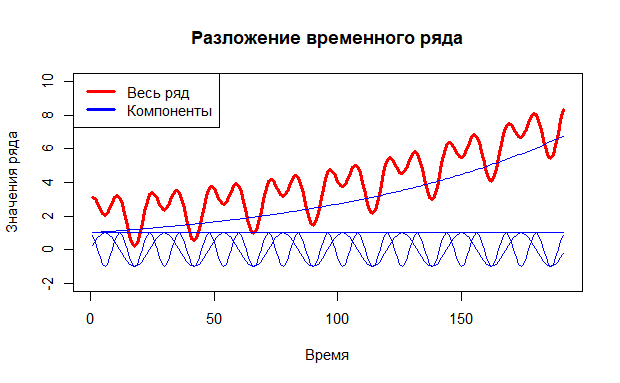
\includegraphics[width=0.8\textwidth]{img/trend inseparability example/all.png}
%	\caption{Правильное разложение ряда $\TS = \TS_c + \TS_e + \TS_{\cos} + \TS_{\sin}$}
%	\label{fig:c_e_cos}
%\end{figure}
%
%\begin{figure}[H]
%	\centering
%	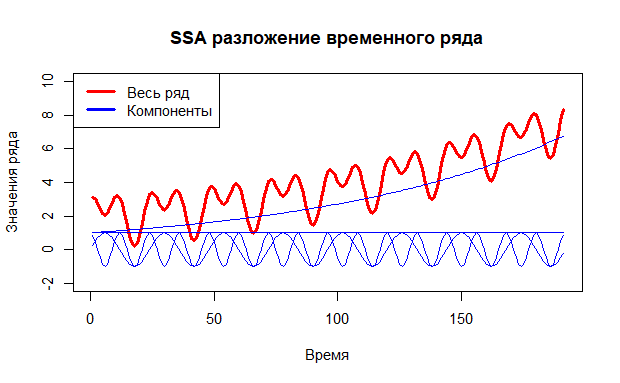
\includegraphics[width=0.8\textwidth]{img/trend inseparability example/ssa.png}
%	\caption{Разложение ряда $\TS = \TS_c + \TS_e + \TS_{\cos} + \TS_{\sin}$ методом $\SSA$}
%	\label{fig:c_e_cos_ssa}
%\end{figure}
%
%Метод $\SSA$ разделил правильно все компоненты друг от друга.
%
%\begin{figure}[H]
%	\centering
%	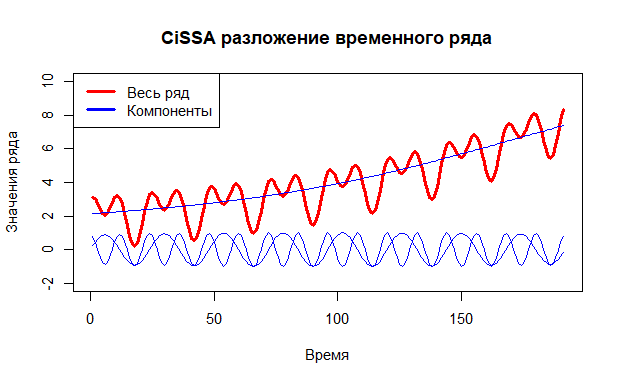
\includegraphics[width=0.8\textwidth]{img/trend inseparability example/cissa.png}
%	\caption{Разложение ряда $\TS = \TS_c + \TS_e + \TS_{\cos} + \TS_{\sin}$ методом $\CISSA$}
%	\label{fig:c_e_cos_cissa}
%\end{figure}
%
%В случае $\CISSA$ получилось так, что экспонента и константа смешались в одну компоненту, одни и те же низкие частоты отвечают за них одновременно, поскольку они не являются периодиками.
%
%% latex table generated in R 4.2.2 by xtable 1.8-4 package
%% Wed Jun 12 06:57:37 2024
%\begin{table}[H]
%	\centering
%	\begin{tabular}{l|lll|llll}
%		\hline
%		Метод/Компонента & $\TS_e$ & $\TS_c$ & $\TS_c + \TS_e$ & $\TS_{\sin}$ & $\TS_{\cos}$ \\ 
%		\hline
%		SSA & 2.2e-25 & 2.2e-25 & 4.2e-28 &3.8e-29 & 1.6e-29 \\ 
%		CiSSA &none & none & 3.5e-02 & 1.4e-04 & 1.9e-03 \\ 
%		\hline
%	\end{tabular}
%	\caption{MSE разложений ряда $\TS = \TS_c + \TS_e + \TS_{\cos} + \TS_{\sin}$ методов $\SSA$ и \CISSA} 
%	\label{tab:errs}
%\end{table}
%
%Таблица \ref{tab:errs} и рисунки \ref{fig:c_e_cos_ssa}, \ref{fig:c_e_cos_cissa} показывают, что метод $\SSA$ справился лучше в сравнении с $\CISSA$, причем как по разделимости, так и по ошибке. В алгоритме $\CISSA$ трендовая составляющая также смешалась с сезонной, поэтому увеличилась ошибка при косинусе. Стоит отметить, что в данном примере использовался алгоритм улучшения разделимости EOSSA \cite{golyandina2023intelligent} для метода $\SSA$. Без него не получились бы такие результаты.
%
%Или же, если заменить $\TS_{e}$ на $\TS_{e \cdot \cos}$, то есть теперь ряд $\TS = \TS_c + \TS_{e \cdot \cos} + \TS_{\cos} + \TS_{\sin} = 1 + e^{\frac{x}{100}} \cos(\frac{2\pi}{48} x) + \cos(\frac{2\pi}{12} x) + \sin(\frac{2\pi}{24} x)$, то получится следующая таблица ошибок:
%\begin{table}[H]
%	\centering
%	\begin{tabular}{l|lllllll}
%		\hline
%		Метод/Компонента & $\TS_{e \cdot \cos}$ & $\TS_{\sin}$ & $\TS_{\cos}$ \\ 
%		\hline
%		SSA & 4.7e-29 & 1.1e-29 & 8.4e-30 \\ 
%		CiSSA  &3.2e-02 & 2.6e-04 & 5.8e-03 \\ 
%		\hline
%	\end{tabular}
%	\caption{MSE разложений ряда $\TS = \TS_c + \TS_{e \cdot \cos} + \TS_{\cos} + \TS_{\sin}$ методов $\SSA$ и \CISSA} 
%	\label{tab:errs_exp_cos}
%\end{table}
%
%Таким образом, таблица \ref{tab:errs_exp_cos} показывает тот же недостаток у метода $\CISSA$, что и таблица \ref{tab:errs}.


\subsection{Выделение тренда}

\label{subsubsec:trend}

Рассмотрим, влияние непериодических компонент на разложение ряда.

Базовый алгоритм $\SSA$ может выделять трендовую составляющую за счет своего адаптивного базиса. Для алгоритмов $\CISSA$ и разложения Фурье нужно применять процедуры расширения временного ряда, чтобы использовать их для выделения тренда.

\textbf{\large{Пример.}} Рассмотрим ряд из примера в секции \ref{subsubsec:exact} и добавим к нему тренд. $\TS = \TS_{c} + \TS_e + \TS_{\sin} + \TS_{\cos} = 1 + e^{\frac{n}{100}} + \sin{\frac{2\pi}{12}n} + \frac{1}{2}\cos{\frac{2\pi}{3}n}$.
%Для каждого алгоритма параметры выбраны таким способом, чтобы получить наилучший результат. 
Кроме того, для всех алгоритмов кроме базового $\SSA$ выделялись периодические компоненты по диапазонам $\left(w \pm \Delta \right)$, где $\Delta = \frac{1}{N+1}$, $w = \frac{1}{12}, \frac{1}{3}$, а непериодичность соответствовала диапазону частот $\left[0, \frac{1}{24} \right)$.
Будем искать экспоненту и константу по низким частотам, назовем это трендовой составляющей ряда.

\begin{table}[H]
	\caption{MSE разложений ряда $\TS = \TS_{c} + \TS_e + \TS_{\sin} + \TS_{\cos}$}
	\centering
	\begin{tabular}{l|l|cccc}
		\hline
		Метод              & Параметры            & $\operatorname{MSE}(\TS_{c} + \TS_e)$ & $\operatorname{MSE}(\TS_{\sin})$ & $\operatorname{MSE}(\TS_{\cos})$ & $\operatorname{MSE}(\TS)$ \\
		\hline
		SSA                & $L = 96, K = 96 $    & 6.1e-05                               & 8.9e-07                          & 5.2e-05                          & 2.1e-28                   \\
		SSA EOSSA, $r = 6$ & $L = 96, K = 96 $    & 1.7e-28                               & 1.6e-29                          & 8.7e-30                          & 1.6e-28                   \\
		Fourier            & $N = 96 \cdot 2$     & 1.1e-01                               & 6.1e-04                          & 6.8e-03                          & 1.1e-01                   \\
		Fourier extended   & $N = 96 \cdot 2$     & 1.4e-03                               & 1.3e-03                          & 8.4e-03                          & 9.6e-03                   \\
		CiSSA              & $L = 96$             & 5.3e-02                               & 1.6e-05                          & 4.9e-04                          & 4.4e-02                   \\
		CiSSA extended     & $L = 96$             & 5.0e-04                               & 2.1e-04                          & 1.1e-03                          & 6.0e-04                   \\
		\hline
		SSA                & $L = 96, K = 97 $    & 7.3e-05                               & 4.2e-06                          & 6.2e-05                          & 1.1e-27                   \\
		SSA EOSSA, $r = 6$ & $L = 96, K = 97 $    & 1.0e-27                               & 2.3e-29                          & 9.7e-30                          & 9.5e-28                   \\
		Fourier            & $N = 96 \cdot 2 - 1$ & 1.2e-01                               & 1.9e-02                          & 2.2e-02                          & 1.0e-01                   \\
		Fourier extended   & $N = 96 \cdot 2 - 1$ & 2.7e-03                               & 3.1e-04                          & 3.1e-03                          & 5.9e-03                   \\
		CiSSA              & $L = 97$             & 7.6e-02                               & 4.1e-02                          & 1.4e-02                          & 1.1e-01                   \\
		CiSSA extended     & $L = 97$             & 5.8e-04                               & 1.3e-02                          & 2.0e-03                          & 1.4e-02                   \\
		\hline
	\end{tabular}
	\label{tab:errs_fourier_cissa_trend}
\end{table}


По таблице \ref{tab:errs_fourier_cissa_trend} видно, что алгоритмы $\CISSA$ и Фурье без модификаций достаточно плохо определяют тренд. Ситуация с выделением тренда улучшается при использовании процедуры расширения ряда, однако есть недостаток у такого решения. В примерах, рассматривающихся  для таблиц \ref{tab:precise_separability_example1} и \ref{tab:errs_fourier_cissa_trend}, можно заметить, что при применении расширения ряда ухудшается отделение периодических составляющих. Подобной проблемы нет с улучшением разделимости в методе $\SSA$.

\subsection{Отделение сигнала от шума}

%НАПИСАТЬ РЕЗУЛЬТАТЫ ПРЕДЫДУЩИХ ПРИМЕРОВ С ШУМОМ. СДЕЛАТЬ ВЫВОДЫ.

Рассмотрим влияние шума на результаты разделимости предыдущих примеров.

\textbf{\large{Пример.}} Вернемся к примеру из секции \ref{subsubsec:exact} и добавим к нему шум: $\TS = \TS_{\sin} + \TS_{\cos} + \TS_{\mathrm{noise}} = \sin{\frac{2\pi}{12}n} + \frac{1}{2}\cos{\frac{2\pi}{3}n} + \varepsilon_n$, где $\varepsilon_n \sim \mathrm N(0, 0.1^2)$.
Кроме того, для всех алгоритмов кроме базового $\SSA$ выделялись периодические компоненты по диапазонам $\left(w \pm \Delta \right)$, где $\Delta = \frac{1}{N+1}$, $w = \frac{1}{12}, \frac{1}{3}$.
Проводилось $100$ тестов, в таблице \ref{tab:errs_fourier_cissa_sin_cos_noised} указаны средние значения ошибки для одних и тех же реализаций шума.
\begin{table}[H]
	\caption{MSE разложений ряда $\TS = \TS_{\sin} + \TS_{\cos} +\TS_{\mathrm{noise}}$ }
	\centering
	\begin{tabular}{l|l|ccc}
		\hline
		Метод              & Параметры            & $\operatorname{MSE}(\TS_{\sin})$ & $\operatorname{MSE}(\TS_{\cos})$ & $\operatorname{MSE}(\TS)$ \\
		\hline
		SSA                & $L = 96, K = 96 $    & 2.9e-04                          & 3.1e-04                          & 5.9e-04                   \\
		SSA EOSSA, $r = 4$ & $L = 96, K = 96 $    & 2.9e-04                          & 3.1e-04                          & 5.9e-04                   \\
		Fourier            & $N = 96 \cdot 2$     & 1.0e-04                          & 1.1e-04                          & 2.2e-04                   \\
		Fourier extended   & $N = 96 \cdot 2$     & 1.2e-03                          & 3.9e-03                          & 5.1e-03                   \\
		CiSSA              & $L = 96$             & 1.6e-04                          & 1.8e-04                          & 3.4e-04                   \\
		CiSSA extended     & $L = 96$             & 6.6e-04                          & 1.9e-03                          & 2.5e-03                   \\
		\hline
		SSA                & $L = 96, K = 97 $    & 2.9e-04                          & 3.1e-04                          & 5.9e-04                   \\
		SSA EOSSA, $r = 4$ & $L = 96, K = 97 $    & 2.9e-04                          & 3.0e-04                          & 5.9e-04                   \\
		Fourier            & $N = 96 \cdot 2 - 1$ & 1.8e-02                          & 7.6e-03                          & 2.6e-02                   \\
		Fourier extended   & $N = 96 \cdot 2 - 1$ & 1.2e-03                          & 8.4e-04                          & 2.0e-03                   \\
		CiSSA              & $L = 97$             & 4.1e-02                          & 1.2e-02                          & 5.2e-02                   \\
		CiSSA extended     & $L = 97$             & 1.4e-02                          & 3.0e-03                          & 1.7e-02                   \\
		\hline
	\end{tabular}
	\label{tab:errs_fourier_cissa_sin_cos_noised}
\end{table}


% Sun Feb 16 18:11:24 2025
%\begin{table}[ht]
%	\centering
%	\begin{tabular}{llll}
%		\hline
%		Метод & sin\_err & cos\_err & all\_err \\ 
%		\hline
%		SSA & 2.9e-04 & 3.1e-04 & 5.9e-04 \\ 
%		SSA EOSSA & 2.9e-04 & 3.1e-04 & 5.9e-04 \\ 
%		Fourier & 1.0e-04 & 1.1e-04 & 2.2e-04 \\ 
%		CiSSA & 1.6e-04 & 1.8e-04 & 3.4e-04 \\ 
%		CiSSA extended & 6.6e-04 & 1.9e-03 & 2.5e-03 \\ 
%		Fourier extended & 1.2e-03 & 3.9e-03 & 5.1e-03 \\ 
%		\hline
%	\end{tabular}
%	\caption{Example Table} 
%\end{table}

По таблице \ref{tab:errs_fourier_cissa_sin_cos_noised} видно, что зашумление ряда сильно повлияло на ошибку, теперь она не является машинным нулем ни для одного из методов. Также был проведен парный t-критерий для зависимых выборок с целью проверки гипотезы о равенстве средних значений ошибки для каждой компоненты, попарно для всех методов. В качестве нулевой гипотезы ($H_0$) предполагалось, что средние значения двух сравниваемых выборок равны. Критический уровень значимости был установлен на уровне $\alpha = 0.05$.
Результаты анализа показали, что во всех случаях, кроме сравнения $\SSA$ и $\SSA$ с EOSSA, $p$-значение оказалось меньше 0.05, что позволяет отвергнуть нулевую гипотезу.

\textbf{\large{Пример.}} Теперь вновь добавим трендовую составляющую к ряду: $\TS = \TS_{c} + \TS_e + \TS_{\sin} + \TS_{\cos} + \TS_{\mathrm{noise}} = 1 + e^{\frac{x}{100}} + \sin{\frac{2\pi}{12}x} + \frac{1}{2}\cos{\frac{2\pi}{3}x} + \varepsilon_n$, где $\varepsilon_n \sim \mathrm N(0, 0.1^2)$. Кроме того, для всех алгоритмов кроме базового $\SSA$ выделялись периодические компоненты по диапазонам $\left(w \pm \Delta \right)$, где $\Delta = \frac{1}{N+1}$, $w = \frac{1}{12}, \frac{1}{3}$, а непериодичность соответствовала диапазону частот $\left[0, \frac{1}{24} \right)$. Проводилось $100$ тестов, в таблице \ref{tab:errs_fourier_cissa_trend_noised} указаны средние значения ошибки для одних и тех же реализаций шума.

\begin{table}[H]
	\caption{MSE разложений ряда $\TS = \TS_{\sin} + \TS_{\cos} + \TS_{c} + \TS_e+\TS_{\mathrm{noise}}$ методов}
	\centering
	\begin{tabular}{l|l|cccc}
		\hline
		Метод              & Параметры          & $\operatorname{MSE}(\TS_{c} + \TS_e)$ & $\operatorname{MSE}(\TS_{\sin})$ & $\operatorname{MSE}(\TS_{\cos})$ & $\operatorname{MSE}(\TS)$ \\
		\hline
		SSA                & $L = 96, K = 96 $  & 5.2e-03                               & 2.9e-04                          & 3.6e-04                          & 5.2e-03                   \\
		SSA EOSSA, $r = 6$ & $L = 96, K = 96 $  & 9.5e-04                               & 2.9e-04                          & 3.1e-04                          & 1.5e-03                   \\
		Fourier            & $N = 96 \cdot 2$   & 1.2e-01                               & 6.9e-04                          & 7.2e-03                          & 1.1e-01                   \\
		Fourier extended   & $N = 96 \cdot 2$   & 3.0e-03                               & 1.9e-03                          & 9.6e-03                          & 1.2e-02                   \\
		CiSSA              & $L = 96$           & 5.5e-02                               & 1.7e-04                          & 7.0e-04                          & 4.6e-02                   \\
		CiSSA extended     & $L = 96$           & 2.7e-03                               & 6.8e-04                          & 2.1e-03                          & 3.1e-03                   \\
		\hline
		SSA                & $L = 96, K = 97 $  &
		5.5e-03            & 2.9e-04            & 3.7e-04                               & 5.3e-03                                                                                         \\
		SSA EOSSA, $r = 6$ & $L = 96, K = 97 $  &
		9.3e-04            & 2.9e-04            & 3.1e-04                               & 1.5e-03                                                                                         \\
		Fourier            & $N = 96 \cdot 2-1$ &
		1.2e-01            & 1.9e-02            & 2.2e-02                               & 1.0e-01                                                                                         \\
		Fourier extended   & $N = 96 \cdot 2-1$ &
		4.7e-03            & 8.6e-04            & 3.0e-03                               & 7.8e-03                                                                                         \\
		CiSSA              & $L = 97$           &
		7.7e-02            & 4.1e-02            & 1.4e-02                               & 1.1e-01                                                                                         \\
		CiSSA extended     & $L = 97$           &
		2.7e-03            & 1.4e-02            & 3.3e-03                               & 1.7e-02                                                                                         \\
		\hline
	\end{tabular}
	\label{tab:errs_fourier_cissa_trend_noised}
\end{table}


Как видно из таблицы \ref{tab:errs_fourier_cissa_trend_noised}, разделения ухудшились, однако $\SSA$ с улучшением разделимости EOSSA отработал лучше всех, а хуже всех показали себя алгоритмы Фурье. Также был проведен был проведён двухвыборочный t-критерий для зависимых выборок с целью проверки гипотезы о равенстве средних значений ошибки для каждой компоненты, попарно для всех методов. В качестве нулевой гипотезы ($H_0$) предполагалось, что средние значения двух сравниваемых выборок равны. Критический уровень значимости был установлен на уровне $\alpha = 0.05$.
Результаты анализа показали, что во всех случаях, кроме сравнения синуса для базового $\SSA$ и $\SSA$ с EOSSA, а также синуса для Фурье и расширенного $\CISSA$, $p$-значение оказалось меньше $0.05$, что позволяет отвергнуть нулевую гипотезу.

Таким образом, можно сделать вывод, что алгоритмы отделяют сигнал от шума примерно одинаково, когда ряд состоит из периодик и параметры правильно подобраны. Результаты не сильно изменяются для базового $\SSA$ и $\SSA$ с EOSSA. Для $\CISSA$ и Фурье результаты ухудшаются. С добавлением трендовой составляющей ситуация меняется: для $\SSA$ результаты практически не ухудшаются, $\CISSA$ с расширением показывает себя немного хуже $\SSA$, остальные алгоритмы выдают значения ошибки на порядки большие.

\subsection{Разделение непериодических составляющих между собой}
\label{subsubsec:nonperiodic}

Как удалось выяснить, все рассматриваемые алгоритмы могут выделять трендовую составляющую из ряда. Однако лишь $\SSA$ способен различить между собой две непериодических компоненты. Про скорость асимптотической разделимости для $\SSA$ можно подробнее узнать в книге \cite{golyandina2001analysis}. Методы $\CISSA$ и Фурье никаким образом не смогут отличить две непериодики между друг другом, поскольку они объединяют компоненты только по частотам. А двум непериодикам соответствуют одинаковые (низкие) наборы частот.


\subsection{Преимущества и недостатки методов SSA, Фурье и CiSSA}
%ДОБАВИТЬ НЕДОСТАЮЩИЕ ПРИМЕРЫ ПО СТОЛБЦАМ, СКАЗАТЬ, КАКИЕ СТОЛБЦЫ УЖЕ С ПРИМЕРАМИ (ИЗ ПРЕДЫДУЩИХ СЕКЦИЙ), СДЕЛАТЬ МИНИ ВЫВОДЫ

Для наглядного отображения преимуществ каждого из этих методов составлены похожие по смыслу таблицы \ref{tab:advantages_ssa_cissa} и \ref{tab:advantages_fourier}, где строки соответствуют методам, а столбцы --- условиям (особым видам компонент ряда). Разделение на две таблицы объяснимо тем, что методам $\SSA$ и $\CISSA$ важно, какие $L$ и  $K$ выбраны у ряда, в то время как разложение Фурье волнует только $N$. На пересечении строк и столбцов указан знак, показывающий, достигается ли разделение компоненты: плюс (+) обозначает точное выполнение, знак стремления указывает на асимптотическое выполнение, а минус (–) --- на отсутствие разделимости.

Обозначения:
\begin{itemize}
	\item $\cos$ --- в ряде присутствуют только периодические компоненты вида $A\cos(2\pi w x + \varphi)$;
	\item $\TS_{\mathrm{np}1}$ --- одна непериодическая компонента в ряде, остальные имеют период;
	\item $\TS_{\mathrm{np}}$ --- несколько непериодических компонент в ряде, остальные имеют период, интересует разделение между
	      непериодическими компонентами;
	\item group --- автоматическая группировка по заданным частотам.
\end{itemize}


\begin{table}[H]
	\caption{Преимущества и недостатки методов $\SSA$, $\CISSA$}
	\centering
	\begin{center}
		\begin{tabular}{l|cccccccc}
			\hline
			Метод/Условие  & $\cos$,             & $\cos$,                & $\cos$,                 & $\TS_{\mathrm{np1}}$ & $\TS_{\mathrm{np}}$ & group \\
			               & $Lw \in \mathbb N$, & $Lw\in \mathbb N$,     & $Lw \not\in \mathbb N$, &                                                    \\
			               & $Kw\in \mathbb N$   & $Kw \not\in \mathbb N$ & $Kw \not\in \mathbb N$  &                                                    \\
			\hline
			SSA            & $+$                 & $\to$                  & $\to$                   & $\to$                & $\to$               & $-$   \\
			SSA EOSSA      & $+$                 & $\to$                  & $\to$                   & $\to$                & $\to$               & $+$   \\
			CiSSA          & $+$                 & $+$                    & $\to$                   & $-$                  & $-$                 & $+$   \\
			CiSSA extended & $+$                 & $+$                    & $\to$                   & $\to$                & $-$                 & $+$   \\
			\hline
		\end{tabular}
	\end{center}
	\label{tab:advantages_ssa_cissa}
\end{table}

\begin{table}[H]
	\caption{Преимущества и недостатки методов Fourier}
	\centering
	\begin{center}
		\begin{tabular}{l|cccccccc}
			\hline
			Метод/Условие    & cos,               & cos,                    & $\TS_{\mathrm{np1}}$ & $\TS_{\mathrm{np}}$ & group \\
			                 & $Nw \in \mathbb N$ & $Nw \not \in \mathbb N$                                                      \\
			\hline
			Fourier          & $+$                & $\to$                   & $-$                  & $-$                 & $+$   \\
			Fourier extended & $+$                & $\to$                   & $\to$                & $-$                 & $+$   \\
			\hline
		\end{tabular}
	\end{center}
	\label{tab:advantages_fourier}
\end{table}



Большинство ситуаций из таблицы \ref{tab:advantages_ssa_cissa} и  \ref{tab:advantages_fourier} уже были разобраны в предыдущих разделах. Так, столбцы, связанные с $\cos$, были разобраны в разделах \ref{subsubsec:exact} и \ref{subsubsec:asymp}. Ситуация с одной непериодической компонентой разобрана в \ref{subsubsec:trend}, а с отделением нескольких непериодик в \ref{subsubsec:nonperiodic}. Автоматическая группировка компонент по заранее заданным частотам в \ref{subsubsec:autogroup}.

Анализ полученных результатов показывает, что $\CISSA$ превосходит разложение Фурье как с расширением ряда, так и без него, во всех случаях, когда интересующие частоты совпадают с частотной решеткой алгоритмов. Если же частоты не совпадают, разложение Фурье может дать лучший результат благодаря более детальному разбиению частот. Кроме того, $\SSA$ с улучшением разделимости EOSSA продемонстрировал более высокую эффективность по сравнению со всеми ранее рассматриваемыми алгоритмами.


%Данные методы разложения временного ряда должны совпадать, если ряд состоит только из периодических компонент. Например, пусть $\TS = \TS_{\sin} + \TS_{\cos} = \sin{\frac{2\pi}{12}x} + \frac{1}{2}\cos{\frac{2\pi}{3}x}$, $L = 96$, $N = 96 \cdot 2$ для разложения Фурье и $N = 96 \cdot 2 - 1$ для остальных, чтобы выполнялись условия выполнения разделимости частот. Сравним результаты по среднеквадратичной ошибке:
%
%\begin{table}[H]
%	\centering
%	\begin{tabular}{l|ccccccl}
%		\hline
%		Метод/Компонента & $\TS_{\sin}$ & $\TS_{\cos}$  & $\TS$\\ 
%		\hline
%		SSA & 6.8e-30 & 1.5e-29 & 1.8e-29 \\ 
%		SSA EOSSA, $r = 4$ & 1.5e-29 & 7.5e-30 & 2.0e-29 \\ 
%		Fourier & 1.7e-28 & 3.5e-28 & 5.1e-28 \\ 
%		Fourier extended & 6.2e-04 & 2.6e-03 & 3.2e-03 \\ 
%		CiSSA & 1.9e-29 & 5.3e-30 & 2.1e-29 \\ 
%		CiSSA extended & 2.0e-04 & 8.6e-04 & 1.1e-03 \\ 
%		\hline
%	\end{tabular}
%	\caption{MSE разложений ряда $\TS = \TS_{\sin} + \TS_{\cos}$} 
%	\label{tab:errs_fourier_cissa_sin_cos}
%\end{table}
%
%%\begin{table}[ht]
%%	\centering
%%	\begin{tabular}{llll}
%%		\hline
%%		Метод & sin\_err & cos\_err & all\_err \\ 
%%		\hline
%%		SSA & 6.8e-30 & 1.5e-29 & 1.8e-29 \\ 
%%		SSA EOSSA & 1.5e-29 & 7.5e-30 & 2.0e-29 \\ 
%%		Fourier & 1.7e-28 & 3.5e-28 & 5.1e-28 \\ 
%%		CiSSA & 1.9e-29 & 5.3e-30 & 2.1e-29 \\ 
%%		CiSSA extended & 2.0e-04 & 8.6e-04 & 1.1e-03 \\ 
%%		Fourier extended & 6.2e-04 & 2.6e-03 & 3.2e-03 \\ 
%%		\hline
%%	\end{tabular}
%%	\caption{Example Table} 
%%\end{table}
%
%
%Таблица \ref{tab:errs_fourier_cissa_sin_cos} показывает, что разложения без расширений ряда сделали правильное (с точностью до вычислений с помощью компьютера) разделение компонент ряда. Однако расширение в методах $\CISSA$ и Фурье ухудшило разделимость периодических частей.
%
%Теперь добавим к этому ряду шум: $\TS = \TS_{\sin} + \TS_{\cos} + \TS_{\mathrm{noise}} = \sin{\frac{2\pi}{12}x} + \frac{1}{2}\cos{\frac{2\pi}{3}x} + \varepsilon_n$, где $\varepsilon_n \sim \mathrm N(0, 0.1)$, $L = 96$, $N = 96 \cdot 2$ для разложения Фурье и $N = 96 \cdot 2 - 1$ для остальных. Результаты должны ухудшиться. Проводилось $100$ тестов, в таблице \ref{tab:errs_fourier_cissa_sin_cos_noised} указаны средние значения ошибки для одних и тех же реализаций шума.
%\begin{table}[H]
%	\centering
%	\begin{tabular}{l|ccc}
%		\hline
%		Метод/Компонента & $\TS_{\sin}$ & $\TS_{\cos}$ & $\TS$\\ 
%		\hline
%		SSA & 2.9e-04 & 3.1e-04 & 5.9e-04 \\ 
%		SSA EOSSA, $r = 4$ & 2.9e-04 & 3.1e-04 & 5.9e-04 \\ 
%		Fourier & 1.0e-04 & 1.1e-04 & 2.2e-04 \\ 
%		Fourier extended  & 1.2e-03 & 3.9e-03 & 5.1e-03 \\ 
%		CiSSA & 1.6e-04 & 1.8e-04 & 3.4e-04 \\ 
%		CiSSA extended & 6.6e-04 & 1.9e-03 & 2.5e-03 \\ 
%		\hline
%	\end{tabular}
%	\caption{MSE разложений ряда $\TS = \TS_{\sin} + \TS_{\cos} +\TS_{\mathrm{noise}}$ } 
%	\label{tab:errs_fourier_cissa_sin_cos_noised}
%\end{table}
%
%
%% Sun Feb 16 18:11:24 2025
%%\begin{table}[ht]
%%	\centering
%%	\begin{tabular}{llll}
%%		\hline
%%		Метод & sin\_err & cos\_err & all\_err \\ 
%%		\hline
%%		SSA & 2.9e-04 & 3.1e-04 & 5.9e-04 \\ 
%%		SSA EOSSA & 2.9e-04 & 3.1e-04 & 5.9e-04 \\ 
%%		Fourier & 1.0e-04 & 1.1e-04 & 2.2e-04 \\ 
%%		CiSSA & 1.6e-04 & 1.8e-04 & 3.4e-04 \\ 
%%		CiSSA extended & 6.6e-04 & 1.9e-03 & 2.5e-03 \\ 
%%		Fourier extended & 1.2e-03 & 3.9e-03 & 5.1e-03 \\ 
%%		\hline
%%	\end{tabular}
%%	\caption{Example Table} 
%%\end{table}
%
%По таблице \ref{tab:errs_fourier_cissa_sin_cos_noised} видно, что зашумление ряда дало негативный эффект на ошибку. Также был проведен парный t-критерий для зависимых выборок с целью проверки гипотезы о равенстве средних значений ошибки для каждой компоненты, попарно для всех методов. В качестве нулевой гипотезы ($H_0$) предполагалось, что средние значения двух сравниваемых выборок равны. Критический уровень значимости был установлен на уровне $\alpha = 0.05$.
%Результаты анализа показали, что во всех случаях, кроме сравнения $\SSA$ и $\SSA$ с EOSSA, $p$-значение оказалось меньше 0.05, что позволяет отвергнуть нулевую гипотезу.
%
%
%Попробуем добавить к ряду непериодическую компоненту. $\TS = \TS_{\sin} + \TS_{\cos} + \TS_{c} + \TS_e = \sin{\frac{2\pi}{12}x} + \frac{1}{2}\cos{\frac{2\pi}{3}x} + 1 + e^{\frac{x}{100}}$, $L = 96$, $N = 96 \cdot 2$ для разложения Фурье и $N = 96 \cdot 2 - 1$. Непериодические компоненты будут отвечать низким частотам. Проблема лишь в том, что с помощью методов разложения Фурье $\CISSA$ невозможно различить между собой две непериодические компоненты, поскольку группировка работает по частотам, элементы разложения неизбежно смешаются между собой. Будем искать экспоненту и константу по низким частотам, назовем это трендовой составляющей ряда. По таблице \ref{tab:advantages_ssa_cissa} лучше всех должен справиться $\SSA$ с улучшением разделимости EOSSA. Хуже всех --- разложение Фурье, поскольку он никаким образом не сможет вычленить из ряда экспоненту.
%
%\begin{table}[H]
%	\centering
%	\begin{tabular}{l|ccccc}
%		\hline
%		Метод/Компонента & $\TS_{c} + \TS_e$ & $\TS_{\sin}$ & $\TS_{\cos}$ & $\TS$\\ 
%		\hline
%		SSA& 5.0e-03 & 8.9e-07 & 5.2e-05 & 4.4e-03 \\ 
%		SSA EOSSA, $r = 7$ & 1.7e-28 & 1.6e-29 & 8.7e-30 & 1.6e-28 \\ 
%		Fourier  & 1.1e-01 & 6.1e-04 & 6.8e-03 & 1.1e-01 \\ 
%		Fourier extended & 1.4e-03 & 1.3e-03 & 8.4e-03 & 9.6e-03 \\ 
%		CiSSA & 5.3e-02 & 1.6e-05 & 4.9e-04 & 4.4e-02 \\ 
%		CiSSA extended & 5.0e-04 & 2.1e-04 & 1.1e-03 & 6.0e-04 \\ 
%		\hline
%	\end{tabular}
%	\caption{MSE разложений ряда $\TS = \TS_{\sin} + \TS_{\cos} + \TS_{c} + \TS_e$ методов} 
%	\label{tab:errs_fourier_cissa_trend}
%\end{table}
%
%% Sun Feb 16 18:31:18 2025
%%\begin{table}[ht]
%%	\centering
%%	\begin{tabular}{lllll}
%%		\hline
%%		Метод & e\_err & sin\_err & cos\_err & all\_err \\ 
%%		\hline
%%		SSA & 5.0e-03 & 8.9e-07 & 5.2e-05 & 4.4e-03 \\ 
%%		SSA EOSSA & 1.7e-28 & 1.6e-29 & 8.7e-30 & 1.6e-28 \\ 
%%		Fourier & 1.1e-01 & 6.1e-04 & 6.8e-03 & 1.1e-01 \\ 
%%		CiSSA & 5.3e-02 & 1.6e-05 & 4.9e-04 & 4.4e-02 \\ 
%%		CiSSA extended & 5.0e-04 & 2.1e-04 & 1.1e-03 & 6.0e-04 \\ 
%%		Fourier extended & 1.4e-03 & 1.3e-03 & 8.4e-03 & 9.6e-03 \\ 
%%		\hline
%%	\end{tabular}
%%	\caption{Example Table} 
%%\end{table}
%
%
%Результаты таблицы \ref{tab:errs_fourier_cissa_trend} повторяют вышеизложенные рассуждения. Также заметно, что периодические компоненты лучше выделились с помощью $\CISSA$ без процедуры расширения ряда в сравнении с $\CISSA$ с расширением.
%
%Теперь добавим шум в предыдущий пример. Результаты всех разложений должны ухудшиться. $\TS = \TS_{\sin} + \TS_{\cos} + \TS_{c} + \TS_e + \TS_{\mathrm{noise}} = \sin{\frac{2\pi}{12}x} + \frac{1}{2}\cos{\frac{2\pi}{3}x} + 1 + e^{\frac{x}{100}} + \mathrm N(0, 0.1)$, $L = 96$, $N = 96 \cdot 2$ для разложения Фурье и $N = 96 \cdot 2 - 1$. Было проведено 100 тестов, в таблице \ref{tab:errs_fourier_cissa_trend_noised} указаны средние значения ошибки.
%
%\begin{table}[H]
%	\centering
%	\begin{tabular}{l|cccc}
%		\hline
%		Метод/Компонента & $\TS_{c} + \TS_e$ & $\TS_{\sin}$ & $\TS_{\cos}$ & $\TS$\\ 
%		\hline
%		SSA & 5.2e-03 & 2.9e-04 & 3.6e-04 & 5.2e-03 \\ 
%		SSA EOSSA, $r = 7$ & 9.5e-04 & 2.9e-04 & 3.1e-04 & 1.5e-03 \\ 
%		Fourier & 1.2e-01 & 6.9e-04 & 7.2e-03 & 1.1e-01 \\ 
%		Fourier extended & 3.0e-03 & 1.9e-03 & 9.6e-03 & 1.2e-02 \\ 
%		CiSSA & 5.5e-02 & 1.7e-04 & 7.0e-04 & 4.6e-02 \\ 
%		CiSSA extended & 2.7e-03 & 6.8e-04 & 2.1e-03 & 3.1e-03 \\ 
%		\hline
%	\end{tabular}
%	\caption{MSE разложений ряда $\TS = \TS_{\sin} + \TS_{\cos} + \TS_{c} + \TS_e+\TS_{\mathrm{noise}}$ методов} 
%	\label{tab:errs_fourier_cissa_trend_noised}
%\end{table}
%
%% Sun Feb 16 18:50:41 2025
%%%%%\begin{table}[ht]
%%%%%	\centering
%%%%%	\begin{tabular}{lllll}
%%%%%		\hline
%%%%%		Метод & exp\_err & sin\_err & cos\_err & all\_err \\ 
%%%%%		\hline
%%%%%		SSA & 5.2e-03 & 2.9e-04 & 3.6e-04 & 5.2e-03 \\ 
%%%%%		SSA EOSSA & 9.5e-04 & 2.9e-04 & 3.1e-04 & 1.5e-03 \\ 
%%%%%		Fourier & 1.2e-01 & 6.9e-04 & 7.2e-03 & 1.1e-01 \\ 
%%%%%		CiSSA & 5.5e-02 & 1.7e-04 & 7.0e-04 & 4.6e-02 \\ 
%%%%%		CiSSA extended & 2.7e-03 & 6.8e-04 & 2.1e-03 & 3.1e-03 \\ 
%%%%%		Fourier extended & 3.0e-03 & 1.9e-03 & 9.6e-03 & 1.2e-02 \\ 
%%%%%		\hline
%%%%%	\end{tabular}
%%%%%	\caption{Example Table} 
%%%%%\end{table}
%
%
%Как видно из таблицы \ref{tab:errs_fourier_cissa_trend_noised}, разделения ухудшились, однако $\SSA$ с улучшением разделимости EOSSA отработал лучше всех. Также был проведен был проведён двухвыборочный t-критерий для зависимых выборок с целью проверки гипотезы о равенстве средних значений ошибки для каждой компоненты, попарно для всех методов. В качестве нулевой гипотезы ($H_0$) предполагалось, что средние значения двух сравниваемых выборок равны. Критический уровень значимости был установлен на уровне $\alpha = 0.05$.
%Результаты анализа показали, что во всех случаях, кроме сравнения синуса для базового $\SSA$ и $\SSA$ с EOSSA, а также синуса для Фурье и расширенного $\CISSA$, $p$-значение оказалось меньше $0.05$, что позволяет отвергнуть нулевую гипотезу.
%
%По результатам данных примеров и таблицы \ref{tab:advantages_ssa_cissa}, можно понять, что $\CISSA$ работает лучше, чем разложение Фурье, как при расширении ряда, так и без него. Однако это не удивительно, ведь разложение Фурье это частный случай $\CISSA$ при $L = N$. А $\SSA$ с улучшением разделимости EOSSA показал себя лучше базового $\SSA$. Таким образом, далее не будем рассматривать разложение Фурье и базовый $\SSA$, остановимся на $\SSA$ с EOSSA, $\CISSA$ с расширением и без него. Кроме того, по умолчанию будет использоваться $\CISSA$ с расширением, если есть непериодичность, и обычный $\CISSA$, если все компоненты периодичны. Также при написании $\SSA$ будет подразумеваться использование $\SSA$ с EOSSA, если нет конкретных указаний.



%\subsection{Точная разделимость}
%Как удалось выяснить, классов точной разделимости больше в базовом алгоритме $\SSA$, однако в случае разделения $\cos$, условия менее жесткие при использовании $\CISSA$.
%
%Проверим на примерах. 
%Возьмем временной ряд, с разложением которого оба алгоритма должны справиться: $\TS = \TS_{C} + \TS_{cos} = 1 + \cos(\frac{2\pi}{12}x)$, $L = 96 \mid 12$, $N = 96 \cdot 2-1$, $K = 96 \mid 12$. Будем считать MSE между настоящими компонентами ряда и вычисленными.
%\begin{table}[H]
%	\centering
%	\begin{tabular}{l|lllllll}
%		\hline
%		Метод/Компонента & $\TS_{C}$ & $\TS_{\cos} $\\ 
%		\hline
%		SSA & 2.1e-30 & 4.9e-30 \\ 
%		CiSSA & 3.6e-31 & 5.2e-30 \\ 
%		
%		\hline
%	\end{tabular}
%	\caption{MSE разложений ряда $\TS = \TS_{C} + \TS_{\cos}$, $\omega K \in \mathbb N$.} 
%	\label{tab:4_2_1}
%\end{table}
%Ошибки таблицы \ref{tab:4_2_1} можно посчитать за погрешность вычислений на компьютере.
%
%Теперь возьмем временной ряд, при котором $\SSA$ должен отработать хуже $\CISSA$: $\TS = \TS_{C} + \TS_{\cos} = 1 + cos(\frac{2\pi}{12}x)$, $L = 96 \mid 12$, $N = 96 \cdot 2+5$, $K = 102 \nmid 12$. Поскольку $K$ не делится на частоту косинуса, условия точной разделимости в $\SSA$ не выполняются. Будем считать MSE между настоящими компонентами ряда и вычисленными.
%\begin{table}[H]
%	\centering
%	\begin{tabular}{l|lllllll}
%		\hline
%		Метод/Компонента & $\TS_{C}$ & $\TS_{\cos} $\\ 
%		\hline
%		SSA & 9.5e-5 & 9.6e-5 \\ 
%		CiSSA & 3.2e-31 & 5.1e-30 \\ 
%		
%		\hline
%	\end{tabular}
%	\caption{MSE разложений ряда $\TS = \TS_{C} + \TS_{\cos}$, $\omega K \not \in \mathbb N$.} 
%	\label{tab:4_2_2}
%\end{table}
%Таким образом, с разделением косинуса от константы лучше справился алгоритм $\CISSA$, поскольку в нем требуется меньше условий на параметры алгоритма.


\subsection{Проверка алгоритмов на реальных данных}
\label{subsubsec:real_dataZz}
%УБРАТЬ ПРО АВТОМАТИЧЕСКУЮ ГРУППИРОВКУ, ОСТАВИТЬ ТОЛЬКО РЕАЛЬНЫЙ ПРИМЕР

Теперь рассмотрим реальные данные --- месячные ряды промышленного производства (Industrial Production, IP), index $2010 = 100$, в США. Данные промышленного производства полезны, поскольку оно указывается в определении рецессии Национальным бюро экономических исследований (NBER), как один из четырех ежемесячных рядов индикаторов, которые необходимо проверять при анализе делового цикла. Выборка охватывает период с января 1970 года по сентябрь 2014 года, поэтому размер выборки составляет $N = 537$. Источником данных является база данных IMF. Эти показатели демонстрируют различные тенденции, сезонность и цикличность (периодические компоненты, которые соответствуют циклам бизнеса). Данные IP также рассматривались в статье \cite{bogalo2020}.
Применим как $\CISSA$ с расширением ряда, так и $\SSA$ с автоматическим определением частот и улучшениями разделимости EOSSA и FOSSA с параметром $r = 30$ по следующим группам:
\begin{enumerate}
	\item Трендовой составляющей должны отвечать низкие частоты, поэтому диапазон: $\left[0, \frac{1}{192}\right]$;
	\item Циклы бизнеса по диапазонам: $\left[\frac{2}{192}, \frac{10}{192}\right]$;
	\item Сезонность по частотам $\omega_k = 1/12, 1/6, 1/4, 1/3, 5/12, 1/2$;
\end{enumerate}
На основе предыдущих требований взято $L = 192$.

\begin{figure}[H]
	\centering
	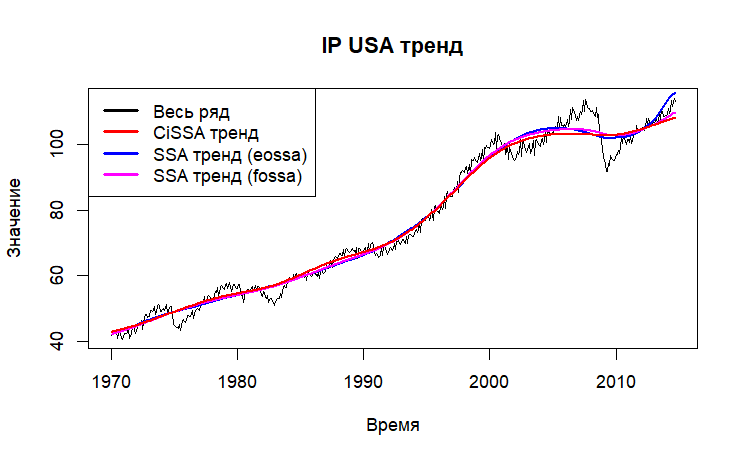
\includegraphics[width=0.8\textwidth]{img/trend inseparability example/IP_trend.png}
	\caption{Трендовая составляющая данных IP USA}
	\label{fig:IP_trend}
\end{figure}

При применении FOSSA улучшения разделимости алгоритм $\SSA$ выделяет тренд довольно похоже с $\CISSA$. Весь график $\SSA$ тренд EOSSA выглядит более изогнутым при визуальном сравнении с остальными.

\begin{figure}[H]
	\centering
	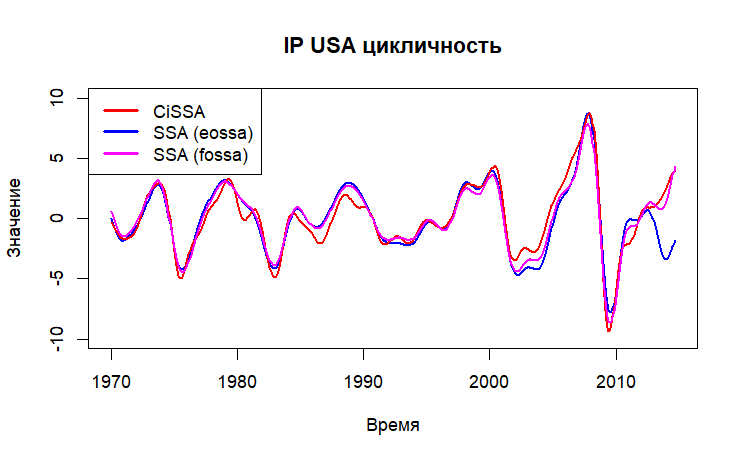
\includegraphics[width=0.8\textwidth]{img/trend inseparability example/IP_cycle.png}
	\caption{Циклическая составляющая данных IP USA}
	\label{fig:IP_cycle}
\end{figure}

Аналогичная тренду ситуация происходит с цикличностью. В случае EOSSA правый хвост (значения ряда после 2010-ого года) смешался между цикличностью и трендом.

\begin{figure}[H]
	\centering
	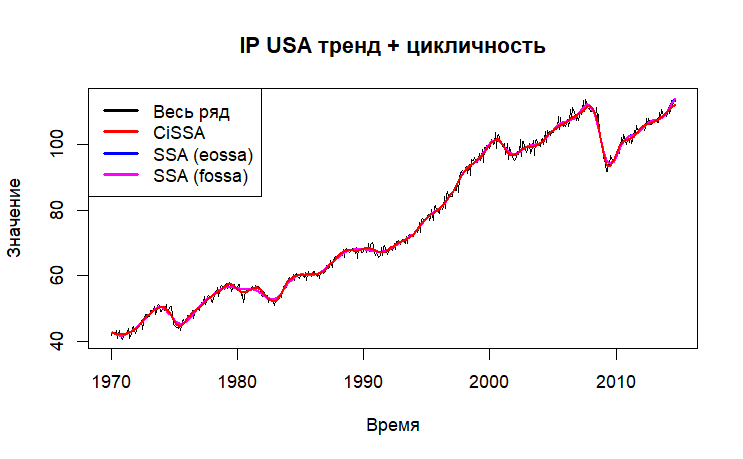
\includegraphics[width=0.8\textwidth]{img/trend inseparability example/IP_trend_sycle.png}
	\caption{Объединение тренда и цикличности IP USA}
	\label{fig:IP_trend_sycle}
\end{figure}

Как видно из графика \ref{fig:IP_trend_sycle}, объединив тренд и цикличность получаем одинаковые результаты для всех рассматриваемых алгоритмов.

\begin{figure}[H]
	\centering
	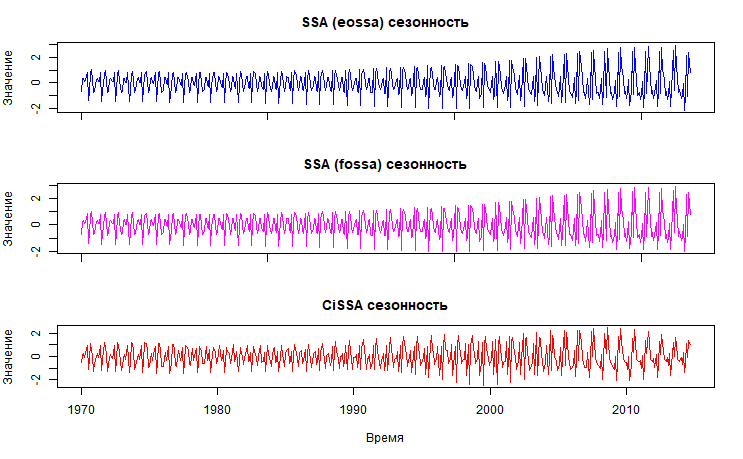
\includegraphics[width=0.8\textwidth]{img/trend inseparability example/IP_sesonal.jpg}
	\caption{Сезонная составляющая данных IP USA}
	\label{fig:IP_sesonal}
\end{figure}

Сезонность выглядит для всех алгоритмов похоже.

%\begin{figure}[H]
%	\centering
%	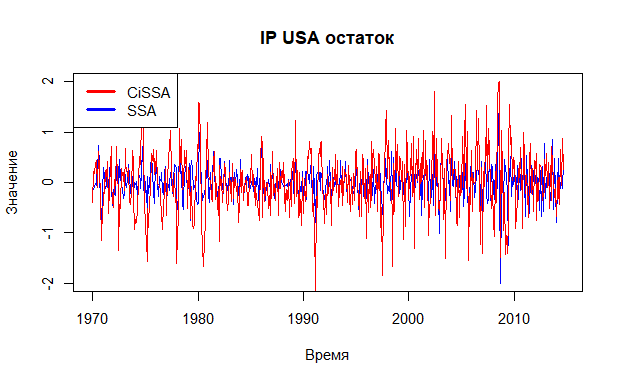
\includegraphics[width=0.8\textwidth]{img/trend inseparability example/IP_residuals.png}
%	\caption{Шум данных IP USA}
%	\label{fig:IP_residuals}
%\end{figure}
Шум же является нормальным во всех случаях.

\begin{figure}[H]
	\centering
	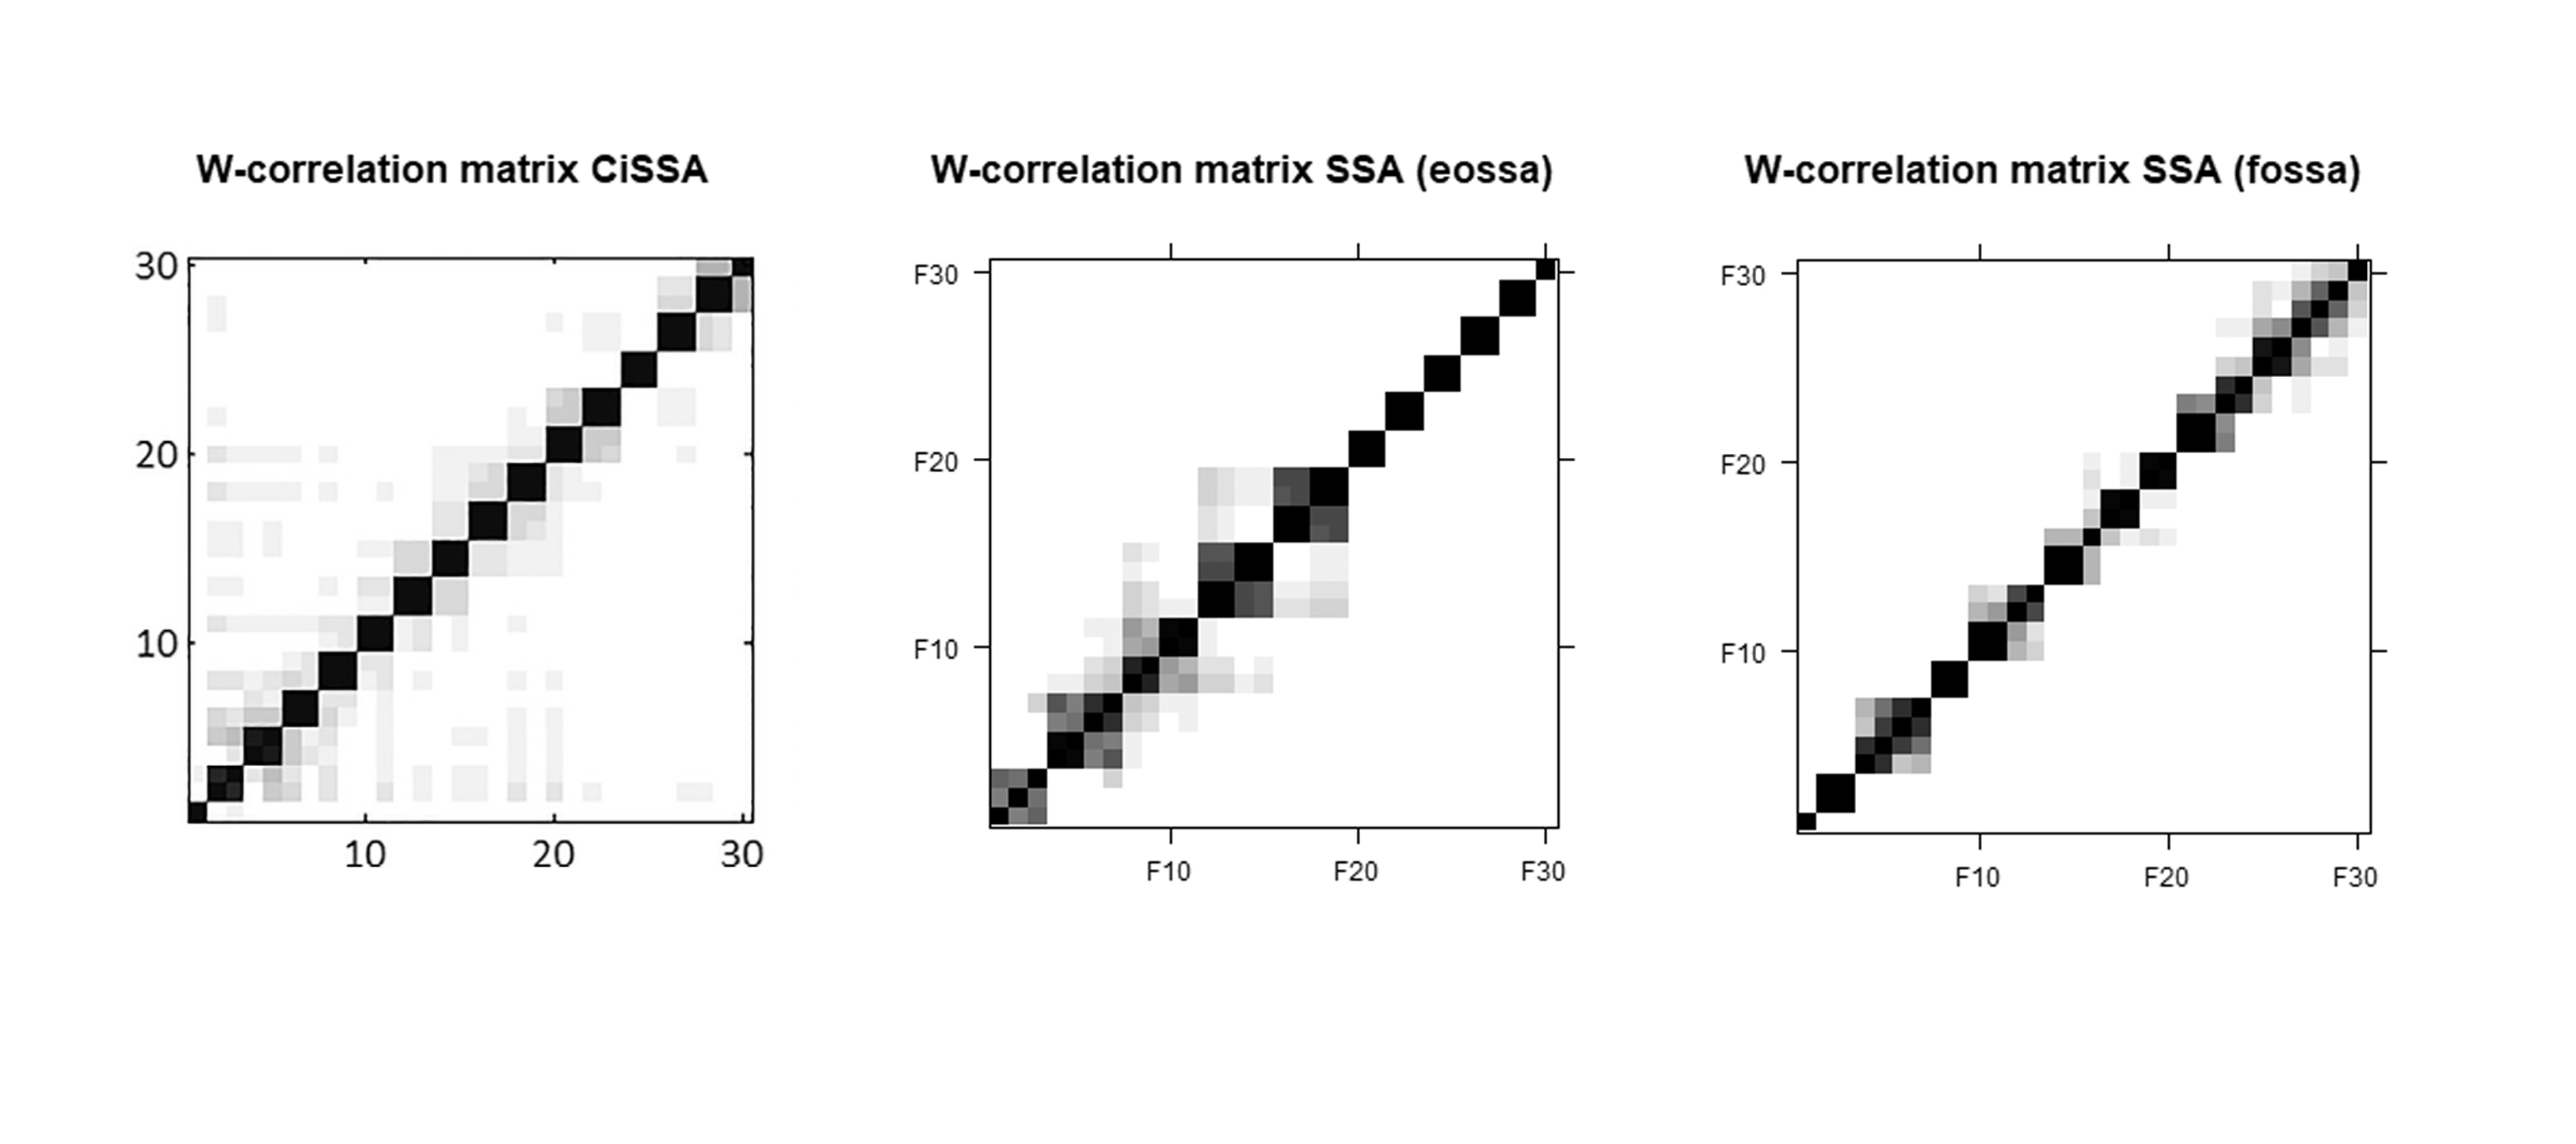
\includegraphics[width=0.8\textwidth]{img/trend inseparability example/W-corr.jpg}
	\caption{Матрицы корреляций IP USA}
	\label{fig:W-corr}
\end{figure}
%TODO: по pdf
По матрицам корреляции заметно, что при использовании $\SSA$ с улучшением разделимости EOSSA, смешиваются первые по значимости компоненты ряда (они и являются трендовыми и циклическими).

%\textbf{ОТСЕБЯТИНА}
%Тренд наиболее гибко и лучше отделяется при применении SSA, цикличность отделилась одинаково в обоих случаях, сезонность выглядит куда приличнее при применении CiSSA. Плюс, приходится подбирать параметры разложения в SSA. В CiSSA вообще ничего не надо делать, просто вкинул, отработало замечательно. 


Таким образом, получились довольно похожие результаты в выделении тренда и цикличности при использовании $\SSA$ с FOSSA и $\CISSA$. Несколько иные результаты при $\SSA$ с EOSSA. Сезонная составляющая для всех алгоритмов выглядит схоже.

\newpage





\section{Многомерные варианты базового SSA}

\label{sec:multidimensional_ssa}

Временные ряды могут быть не только одномерными, но и многомерными, то есть представлять собой наборы связанных наблюдений. В данной работе рассматриваются две модификации базового $\SSA$:
$\MSSA$ и $\DSSA$.

Под многомерным временным рядом будем понимать систему $s$ одномерных временных рядов $\TS = (\TS^{(1)}, \ldots, \TS^{(s)})$, где каждый ряд $\TS^{(p)} = (x_1^{(p)}, \ldots, x_{N_p}^{(p)})$ представляет собой последовательность числовых значений.

Под двумерным рядом будем понимать прямоугольную матрицу $\TS = [x_{ij}] \in \mathbb{R}^{N_x \times N_y}$, содержащую наблюдения, упорядоченные по двум пространственным или иным измерениям (например, изображение).

% Каждый из методов -- $\MSSA$ и $\DSSA$ -- использует свою стратегию формирования траекторной матрицы и, соответственно, имеет особенности в разложении, реконструкции и прогнозировании. Далее будут подробно рассмотрены обе эти модификации SSA, их алгоритмы, интерпретации и примеры применения.


\subsection{MSSA}

Рассмотрим многомерный временной ряд, то есть набор $\{\mathbb{X}^{(p)} = \left({x^{(p)}_{j}}\right) _{j=1}^{N_p}, \; p = 1, \ldots, s\}$ из $s$ временных рядов длины $N_p$, где $p = 1, \ldots, s$.

Обозначим $\mathbb{X} = (\mathbb{X}^{(1)}, \ldots, \mathbb{X}^{(s)})$ как исходные данные для алгоритма $\MSSA$ \cite{ssa_with_R}. Общая схема алгоритма базового $\SSA$. Необходимо лишь определить оператор вложения $\mathcal{J}_{\text{\MSSA}}(\mathbb{X}) = \mathbf X$.

\subsubsection{Вложение}

Пусть $L$ -- длина окна, $1 < L < \min(N_p, \; p = 1, \ldots, s)$. Для каждого временного ряда $\TS^{(p)}$ формируем $K_p = N_p - L + 1$ векторов $\mathbf{X}_j^{(p)} = (x_j^{(p)}, \ldots, x_{j+L-1}^{(p)})^T$, где $1 \leq j \leq K_p$. Обозначим $K = \sum_{p=1}^s K_p$. Траекторная матрица многомерного ряда $\TS$ — это матрица размера $L \times K$ следующего вида:

\[
	\mathcal{J}_{\text{MSSA}}(\TS) = \mathbf{X} = [\mathbf{X}_1^{(1)} : \ldots : \mathbf{X}_{K_1}^{(1)} : \ldots : \mathbf{X}_1^{(s)} : \ldots : \mathbf{X}_{K_s}^{(s)}] = [\mathbf{X}^{(1)} : \ldots : \mathbf{X}^{(s)}],
\]

где $\mathbf{X}^{(p)} = \mathcal{J}_{\text{SSA}}(\TS^{(p)})$ — траекторная матрица одномерного ряда $\TS^{(p)}$. Таким образом, траекторная матрица системы временных рядов имеет блочно-ганкелеву структуру. Заметим, что

\[
	\mathcal{J}^{-1}_{\text{MSSA}}(\mathbf{X}) = [\mathcal{J}^{-1}_{\text{SSA}}(\mathbf{X}^{(1)}) : \ldots : \mathcal{J}^{-1}_{\text{SSA}}(\mathbf{X}^{(s)})].
\]



\subsubsection{Вложение}

Аналогично базовому $\SSA$.

\subsubsection{Группировка}

Аналогично базовому $\SSA$.

\subsubsection{Диагональное усреднение}

Аналогично базовому $\SSA$ \eqref{eq:ssa_projector} определим оператор проектирования для $\MSSA$:

\[
	\Pi_{\text{stacked } \mathcal{H}}(\mathbf{Y}) = [\Pi_{\mathcal{H}}(\mathbf{Y}^{(1)}) : \ldots : \Pi_{\mathcal{H}}(\mathbf{Y}^{(i)})]
\]

Тогда получаем восстановление с помощью $\mathcal{J}_{\text{MSSA}}^{-1} \circ \Pi_{\text{stacked }}$.




\subsubsection{Комментарии}


Собственные векторы $U_i$ из SVD траекторной матрицы $\mathrm{X} = \sum_i \sqrt{\lambda_i} U_i V_i^{\mathsf{T}}$ формируют общее базисное пространство для всех временных рядов. Векторы факторов $V_i$ содержат подкомпоненты $V_i^{(p)}$, соответствующие каждому ряду:

\begin{equation*}
	V_i = \begin{pmatrix} V_i^{(1)} \\ \vdots \\ V_i^{(s)} \end{pmatrix},
\end{equation*}

где $V_i^{(p)} \in \mathbb{R}^{K_p}$ принадлежит строковому пространству $p$-го ряда. $U_i$ отражают общую структуру, $V_i^{(p)}$ — её проявление в отдельных рядах.


Кроме того, $\MSSA$ позволяет вычленить дополнительную информацию про структуру рядов, рассматривая их совместно.



\subsection{2d-ssa}

$\DSSA$ -- это расширение базового $\SSA$ для двумерных массивов \cite{ssa_with_R} (например, изображений). Данные представляются в виде матрицы:
\[
	\TS = (x_{ij})_{i,j=1}^{N_x, N_y}, \quad \text{где } N_x \times N_y \text{ — размер массива.}
\]

Параметрами метода являются размеры {окна} $(L_x, L_y)$, где $1 \leq L_x \leq N_x$, $1 \leq L_y \leq N_y$.

\subsubsection{Вложение}

Как и в $\MSSA$, нужно определить лишь $\mathcal{J}_{\text{2D-SSA}}$

\begin{enumerate}
	\item Из массива $\TS$ выделяются {все возможные подматрицы} размера $L_x \times L_y$ с помощью скользящего окна.
	\item Каждая подматрицы $\TS_{k,l}^{(L_x, L_y)}$ преобразуется в столбец: $\mathbf{X}_{k+(l-1)K_x} = \text{vec}(\TS_{k,l}^{(L_x, L_y)})$.
	\item Траекторная матрица строится как объединение этих столбцов:
	      \[
		      \mathcal{J}_{\text{2D-SSA}}(\TS) = \mathbf{X} = [\mathbf{X}_1 : \ldots : \mathbf{X}_{K_x K_y}].
	      \]
\end{enumerate}

Матрица $\mathbf{X}$ имеет {блочно-ганкелеву структуру}:
\[
	\mathbf{X} =
	\begin{pmatrix}
		\mathbf{H}_1     & \mathbf{H}_2       & \ldots & \mathbf{H}_{K_y}   \\
		\mathbf{H}_2     & \mathbf{H}_3       & \ldots & \mathbf{H}_{K_y+1} \\
		\vdots           & \vdots             & \ddots & \vdots             \\
		\mathbf{H}_{L_y} & \mathbf{H}_{L_y+1} & \ldots & \mathbf{H}_{N_y}
	\end{pmatrix},
\]
где каждая $\mathbf{H}_j$ — ганкелевская матрица, построенная из столбцов $\TS$.

\subsubsection{Вложение}

Аналогично базовому $\SSA$.

\subsubsection{Группировка}

Аналогично базовому $\SSA$.

\subsubsection{Диагональное усреднение}

Аналогично базовому $\SSA$, только восстановление производится по соответствующим ганкелевым блокам матрицы $\mathbf{X}$.

\subsubsection{Комментарии}

{Связь с $\MSSA$:} если $L_x = 1$ или $L_y = 1$, $\DSSA$ эквивалентен $\MSSA$ для временных рядов одинаковой длины. Поэтому его можно назвать обобщением $\MSSA$.

Также при применении $\DSSA$ важен порядок следования строк и столбцов в $\TS$, в отличие от $\MSSA$.



\newpage



\section{Метод Functional singular spectrum analysis (FSSA)}
\label{sec:fssa}

Functional SSA -- метод, предложенный для анализа функциональных временных рядов \cite{haghbin2019functionalsingularspectrumanalysis}. Предлагается объединить теорию многомерного функционального анализа главных компонент (MFPCA) и SSA.

Авторы метода $\FSSA$ сравнивают его с $\MSSA$ и динамическим функциональным анализом главных компонент (dFPCA), показывая преимущество использования $\FSSA$ результаты в разделении компонент функциональных данных, особенно для нестационарных рядов.

В данном разделе преимущественно используются обозначения из статьи \cite{haghbin2019functionalsingularspectrumanalysis}авторов метода 





Рассмотрим, основные определения.

\begin{itemize}
    \item \textbf{Функциональный временной ряд:} $\textbf{y}_N=(y_1,\ldots,y_N)^\top$, длина $N$, $y_i:[0,1]\to\mathbb{R}$, $y_i\in\mathbb{H}=\mathcal{L}^2([0,1])$ с $\langle x,y\rangle=\int_0^1 x(s)y(s)ds$.

    \item \textbf{Пространство $\mathbb{H}^k$:} Декартово произведение $k$ копий $\mathbb{H}$. \\ Элемент ${\pmb x}\in\mathbb{H}^k$: ${\pmb x}(s)=\begin{pmatrix} x_1(s),\ldots,x_k(s)\end{pmatrix}^\top$, $x_i\in\mathbb{H}$, $s\in[0,1]$. Скалярное произведение: $\langle\pmb x,\pmb y\rangle_{\mathbb{H}^k}=\sum_{i=1}^k\langle x_i,y_i\rangle$.

    \item \textbf{Тензорное произведение:} Для $x\in\mathbb{H}_1$, $y\in\mathbb{H}_2$, оператор $x\otimes y:\mathbb{H}_1\to\mathbb{H}_2$, $(x\otimes y)h=\langle x,h\rangle y$, $h\in\mathbb{H}_1$.

    \item \textbf{Пространство $\mathbb{H}^{L\times K}$:} Линейное пространство операторов $\mathcal{Z}:\mathbb{R}^K\to\mathbb{H}^L$, заданных $[z_{i,j}]_{i=1,\ldots,L}^{j=1,\ldots,K}$,
    \begin{equation}\label{eq: z operator}
        \mathcal{Z}\pmb{a}=\begin{pmatrix} \sum_{j=1}^K a_j z_{1,j} \\ \vdots \\ \sum_{j=1}^K a_j z_{L,j} \end{pmatrix}, \ z_{i,j}\in\mathbb{H}, \ \pmb{a}=(a_1,\ldots,a_K)\in\mathbb{R}^K.
    \end{equation}

\end{itemize}






\subsection{Алгоритм FSSA}
Алгоритм сильно схож с базовым $\SSA$.

Для целого числа $1\leq L\leq{N}/{2}$ положим $K=N-L+1$ и определим множество многомерных функциональных векторов в $\mathbb{H}^L$ как
\begin{equation}\label{flvec}
	{\pmb x}_j(s):= \begin{pmatrix} y_j(s), y_{j+1}(s), \ldots, y_{j+L-1}(s)\end{pmatrix}^\top,\ \ j=1,\ldots, K,
\end{equation}
где ${\pmb x}_j$ обозначают функциональные $L$-сдвинутые векторы. Следующий алгоритм предоставляет результаты FSSA в четыре этапа.

\subsubsection{Вложение}
Траекторный оператор $\mathcal{X}:\mathbb{R}^K \rightarrow \mathbb{H}^L$.
\begin{equation}
	\label{eq:traj}
	\mathcal{X}{\pmb a}:=\sum_{j=1}^K a_j{\pmb x}_j=
	\begin{pmatrix} \sum_{j=1}^K a_jy_j\\ \sum_{j=1}^K a_j y_{j+1}\\ \vdots\\ \sum_{j=1}^K a_j y_{j+L-1} \end{pmatrix},
	\ {\pmb a}=\left(a_1,\ldots, a_K\right)^\top \in\mathbb{R}^K.
\end{equation}
 
Кроме того, $\mathcal{X}=\mathcal{T}\textbf{y}_N$, где $\mathcal{T}$ — оператор из $\mathbb{H}^N$ в $\mathbb{H}_H^{L\times K}$. Вычисление $\mathcal{X} \pmb{a}$ в заданной точке $s\in [0,1]$ эквивалентно матричному произведению ${\bf X}(s)\pmb{a}$, где ${\bf X}(s)$ — это $L \times K$ ганкелева матрица, заданная как
\begin{equation}\label{ftraj}
	{\bf X}(s)=\begin{bmatrix} {\pmb x}_1(s), \ldots, {\pmb x}_K(s) \end{bmatrix}.
\end{equation}


Оператор $\mathcal{X}$ является ограниченным линейным оператором. Если определить $\mathcal{X}^*:\mathbb{H}^L \rightarrow \mathbb{R}^K$ как
\begin{equation}
	\mathcal{X}^*{\pmb z}=
	\begin{pmatrix} \sum_{i=1}^L \langle y_i, z_i\rangle\\ \sum_{i=1}^L \langle y_{i+1}, z_i\rangle\\ \vdots\\ \sum_{i=1}^L \langle y_{i+K-1}, z_i\rangle \end{pmatrix},
	\ {\pmb z}=\left(z_1,\ldots, z_L\right)^\top\in\mathbb{H}^L,
\end{equation}
то $\mathcal{X}^*$ является сопряжённым оператором для $\mathcal{X}$.

\subsubsection{Разложение}
Определим оператор $\mathcal{S}: \mathbb{H}^L\rightarrow \mathbb{H}^L$ как $\mathcal{S}:=\mathcal{X}\mathcal{X}^*$. Следовательно, для заданного ${\pmb z}\in \mathbb{H}^{L}$ это означает, что
\begin{align}\label{eq: s-operator}
	\mathcal{S}{\pmb z} &
	=\sum_{j=1}^K\sum_{i=1}^L \langle y_{i+j-1} , z_i \rangle {\pmb x}_j
	=\sum_{j=1}^K \langle {\pmb x}_j , {\pmb z} \rangle_{\mathbb{H}^L} {\pmb x}_j
	=\sum_{j=1}^K ({\pmb x}_j \otimes {\pmb x}_j) {\pmb z}.
\end{align}



Для любого положительного $i$ определим оператор $\mathcal{X}_i:\mathbb{R}^K\rightarrow\mathbb{H}^L$, заданный как
\begin{equation}\label{eq: elementary oprator}
	\mathcal{X}_i \pmb{a}:=\sum_{j=1}^K a_j (\pmb{\psi}_i\otimes \pmb{\psi}_i){\pmb x}_j= (\pmb{\psi}_i\otimes \pmb{\psi}_i)\sum_{j=1}^K a_j{\pmb x}_j.
\end{equation}

$\mathcal{X}_i$ -- элементарный оператор. Вычисление $\mathcal{X}_i \pmb{a}$ в заданной точке $s\in [0,1]$ эквивалентно матричному произведению ${\bf X}_i(s)\pmb{a}$, где ${\bf X}_i(s)$ — это $L \times K$ матрица, заданная как
\begin{align}\label{eq:elementary mat}
	{\bf X}_i(s) & :=
	\begin{bmatrix} \langle\pmb{\psi}_i, {\pmb x}_1\rangle_{\mathbb{H}^L} \pmb{\psi}_i(s), \ldots, \langle\pmb{\psi}_i, {\pmb x}_K\rangle_{\mathbb{H}^L} \pmb{\psi}_i(s) \end{bmatrix}
	\notag            \\ &\ =
	\begin{bmatrix} (\pmb{\psi}_i\otimes \pmb{\psi}_i){\pmb x}_1(s), \ldots, (\pmb{\psi}_i\otimes \pmb{\psi}_i){\pmb x}_K(s) \end{bmatrix}.
\end{align}

% Заметим, что ${\bf X}_i(s)$ можно рассматривать как функциональное расширение элементарных матриц, определённых в \eqref{eq: primary}, где ${\bf X}_i(s)$ проецирует столбцы ${\bf X}(s)$ в пространство, порождённое $\pmb{\psi_i}(s)$.


Элементарные операторы $\mathcal{X}_i$ являются ограниченными операторами ранга один. Кроме того, $\mathcal{X}_i$ декомпозируют траекторный оператор $\mathcal{X}$ как
\begin{equation}\label{eq:elementary operators}
	\mathcal{X}=\sum_{i=1}^\infty \mathcal{X}_i.
\end{equation}

Следующая теорема предоставляет сингулярное разложение (SVD) траекторного оператора $\mathcal{X}$ для получения соответствующих собственных троек ($\sqrt{\lambda_i}, \pmb{v}_i, \pmb{\psi}_i$) на этапе декомпозиции \cite{haghbin2019functionalsingularspectrumanalysis}.
\begin{theorem}
	\label{thm:svd}
	Пусть ${\{\pmb{\psi}_i\}_{i=1}^\infty}$ и ${\{\lambda_i\}_{i=1}^\infty}$ — собственные элементы $\mathcal{S}$, и
	\begin{equation}
		\mathcal{S}^\dag:=\mathcal{X}^*\mathcal{X}=
		\begin{bmatrix}
			\sum_{i=1}^L\langle y_i, y_{i}\rangle       & \cdots & \sum_{i=1}^L\langle y_i, y_{i+K-1}\rangle       \\
			\vdots                                      & \ddots & \vdots                                          \\
			\sum_{i=1}^L\langle y_{i+K-1}, y_{i}\rangle & \cdots & \sum_{i=1}^L\langle y_{i+K-1}, y_{i+K-1}\rangle \\
		\end{bmatrix}.
	\end{equation}
	Тогда сингулярное разложение траекторного оператора $\mathcal{X}$ можно записать как
	\begin{equation}
		\label{eq: svd}
		\mathcal{X} = \sum_{i=1}^\infty \sqrt{\lambda_i}\textbf{v}_i\otimes \pmb{\psi}_i,
	\end{equation}
	где
	$\textbf{v}_i=
		\begin{pmatrix} \frac{\langle\pmb{\psi}_i, {\pmb x}_1\rangle_{\mathbb{H}^L}}{\sqrt{\lambda_i}} , \ldots,\frac{ \langle\pmb{\psi}_i, {\pmb x}_K\rangle_{\mathbb{H}^L}}{\sqrt{\lambda_i}} \end{pmatrix}^\top$. Кроме того, для любого $\pmb{a}\in\mathbb{R}^K$, используя \eqref{eq: svd}, мы имеем
	\begin{equation}
		\mathcal{X}\pmb{a} = \sum_{i=1}^\infty \sqrt{\lambda_i} \langle \textbf{v}_i, \pmb{a}\rangle_{\mathbb{R}^K} \pmb{\psi}_i,
	\end{equation}
	где
	\begin{itemize}
		\item[i)] $\{\lambda_i\}_{i=1}^\infty$ — множество неубывающих собственных значений $\mathcal{S}^\dag$, и
		\item[ii)] $\pmb{v}_i$ — соответствующие ортонормированные собственные векторы $\mathcal{S}^\dag$, удовлетворяющие $\mathcal{X}\pmb{v}_i = \sqrt{\lambda_i} \pmb{\psi}_i$.
	\end{itemize}
\end{theorem}

\subsubsection{Группировка}

Аналогично базовому $\SSA$. Получается 
\begin{equation}\label{eq:grouping}
	\mathcal{X}=\mathcal{X}_{I_1}+\mathcal{X}_{I_2}+\cdots+\mathcal{X}_{I_m}.
\end{equation}


\subsubsection{Диагональное усреднение}

Для заданного $q$ ($1\leq q\leq m$) используется $\mathcal{T}^{-1}:\mathbb{H}_H^{L\times K}\to\mathbb{H}^N$ для преобразования оператора $\mathcal{X}_{I_q}$ из \eqref{eq:grouping} в $\tilde{\bf y}_N^q$. 

Поскольку $\mathcal{X}_{I_q}\in\mathbb{H}^{L\times K}$, сначала выполняется проекция на $\mathbb{H}_H^{L\times K}$, замкнутое подпространство $\mathbb{H}^{L\times K}$. 

Элементы $\mathcal{X}_{I_q}$ и $\tilde{\mathcal{X}}_{I_q}$ обозначаются $[x_{i,j}^{q}]$ и $[\tilde{x}_{i,j}^{q}]$. Метод диагонального усреднения  обобщается на $\mathbb{H}^{L\times K}$, где
\begin{equation}\label{fdiag-ave}
\tilde{x}_{i,j}^{q}=\frac{1}{n_s}\sum_{(l,k): l+k=s} x_{l,k}^q,
\end{equation}
$s=i+j$, $n_s$ — число пар $(l,k)$, таких что $l+k=s$. Проекция обозначается $\Pi_\mathbb{H}:\mathbb{H}^{L\times K}\to\mathbb{H}_H^{L\times K}$, и $\tilde{\mathcal{X}}_{I_q}=\Pi_\mathbb{H} \mathcal{X}_{I_q}$. 

Как итог: $\tilde{\bf y}_N^q=\mathcal{T}^{-1}\tilde{\mathcal{X}}_{I_q}$.




\subsection{Разделимость}\label{subsec: Separability}

Рассматривается $\textbf{y}_N=\textbf{y}_N^{(1)}+\textbf{y}_N^{(2)}$, где $\textbf{y}_N^{(i)}=\{y_1^{(i)},\ldots,y_N^{(i)}\}$, $i=1,2$, — функциональные временные ряды (FTS). Для фиксированной длины окна $L$ для каждого ряда $\textbf{y}_N^{(i)}$ обозначается $\{{\pmb x}_{k}^{(i)}\}_{k=1}^K$ — последовательность функциональных сдвинутых векторов, $\mathcal{L}^{(i)}$ — линейное пространство, порождённое $\{{\pmb x}_{k}^{(i)}\}_{k=1}^K$. Разделимость рядов $\textbf{y}_N^{(1)}$ и $\textbf{y}_N^{(2)}$ эквивалентна $\mathcal{L}^{(1)}\bot\mathcal{L}^{(2)}$, то есть $\langle {\pmb x}_{k}^{(1)},{\pmb x}_{k^\prime}^{(2)}\rangle_{\mathbb{H}^L}=0$ для всех $k,k^\prime=1,\ldots,K$. 

Необходимое условие разделимости определяется через w-корреляцию. Взвешенное скалярное произведение рядов $\textbf{y}_N^{(1)}$ и $\textbf{y}_N^{(2)}$ задаётся как
\begin{equation}\label{winn}
	\langle \textbf{y}_N^{(1)},\textbf{y}_N^{(2)}\rangle_w=\sum_{i=1}^N w_i \langle y_i^{(1)},y_i^{(2)}\rangle,
\end{equation}
где $w_i=\min\{i,L,N-i+1\}$. Ряды $\textbf{y}_N^{(1)}$ и $\textbf{y}_N^{(2)}$ называются w-ортогональными, если
\begin{equation}
	\langle \textbf{y}_N^{(1)},\textbf{y}_N^{(2)}\rangle_w=0.
\end{equation}

\begin{theorem}\label{thm:fSep}
Разделимость рядов $\textbf{y}_N^{(1)}$ и $\textbf{y}_N^{(2)}$ влечёт их w-ортогональность \cite{haghbin2019functionalsingularspectrumanalysis}.
\end{theorem}


% \begin{table}[ht]
% \centering
% \begin{tabular}{cc|ccc|ccc|ccc}
% \toprule
% $\omega$ & $N$ & \multicolumn{3}{c|}{2d-SSA} & \multicolumn{3}{c|}{MSSA} & \multicolumn{3}{c}{FSSA} \\
%         &     & $L=20$ & $L=30$ & $L=40$  & $L=20$ & $L=30$ & $L=40$ & $L=20$ & $L=30$ & $L=40$ \\
% \midrule
% \multirow{4}{*}{0.00} 
% & 50  & 0.092 & 0.026 & 0.022& 0.026 & 0.022 & 0.019 & 0.010 & 0.011 & 0.014 \\
% & 100 & 0.088 & 0.024 & 0.020& 0.026 & 0.022 & 0.018 & 0.008 & 0.007 & 0.007 \\
% & 150 & 0.074 & 0.024 & 0.020& 0.026 & 0.022 & 0.017 & 0.006 & 0.006 & 0.006 \\
% & 200 & 0.071 & 0.024 & 0.019& 0.026 & 0.022 & 0.017 & 0.006 & 0.006 & 0.006 \\
% \midrule
% \multirow{4}{*}{0.10} 
% & 50  & 0.062 & 0.028 & 0.024 & 0.022& 0.026 & 0.022 & 0.009 & 0.011 & 0.014 \\
% & 100 & 0.045 & 0.027 & 0.022 & 0.019& 0.026 & 0.022 & 0.006 & 0.007 & 0.008 \\
% & 150 & 0.037 & 0.027 & 0.020 & 0.019& 0.026 & 0.022 & 0.005 & 0.005 & 0.005 \\
% & 200 & 0.033 & 0.026 & 0.020 & 0.018& 0.026 & 0.022 & 0.005 & 0.005 & 0.005 \\
% \midrule
% \multirow{4}{*}{0.25} 
% & 50  & 0.046 & 0.028 & 0.024 & 0.022& 0.026 & 0.022 & 0.009 & 0.011 & 0.014 \\
% & 100 & 0.040 & 0.027 & 0.022 & 0.020& 0.026 & 0.022 & 0.007 & 0.007 & 0.007 \\
% & 150 & 0.032 & 0.027 & 0.022 & 0.019& 0.026 & 0.022 & 0.006 & 0.006 & 0.005 \\
% & 200 & 0.030 & 0.026 & 0.022 & 0.019& 0.026 & 0.022 & 0.005 & 0.005 & 0.005 \\
% \bottomrule
% \end{tabular}
% \caption{Результаты сравнения методов dFPCA, MSSA и FSSA при различных параметрах $\omega$ и $N$}
% \end{table}


\newpage

\section{Сравнение FSSA, MSSA, 2d-SSA}

\label{sec:compare_fssa_ssa}

В оригинальной работе $\FSSA$ \cite{haghbin2019functionalsingularspectrumanalysis} рассматривалось сравнение алгоритма с dFPCA, $\MSSA$. Однако, $\DSSA$ в данном сравнении не было, хотя он может показать результаты лучше, чем $\MSSA$, за счет того, что более гибко можно рассматривать зависимость по второй переменной. 


\subsection{Численное сравнение}

Рассматриваются функциональные временные ряды длины $N=50, 100, 150$ и $200$, наблюдаемые в $n=100$ фиксированных равноудаленных дискретных точках на $[0,1]$ по следующей модели:
\begin{equation}\label{eq:mainmodel}
Y_t\left(s_i\right)=m_t(s_i)+X_t\left(s_i\right),\ s_i \in [0,1], i=1,\ldots,n, \text{и } t=1, \dots, N.
\end{equation}
Для преобразования $\{Y_t(s_i)\}$ в гладкие (непрерывные) функциональные кривые применяется кубическая B-сплайн базисная функция с 15 степенями свободы. В данной модели $m_t(s)$ является периодической компонентой, определенной как
\begin{equation}\label{eq:Trend}
m_t(s)=e^{s^2} \cos\left(2\pi \omega t\right)+\cos(4\pi s) \sin\left(2\pi \omega t\right),
\end{equation}
где $\omega$ — частота модели с тремя значениями ($\omega=0, 0.1$ и $0.25$).

В этом случае $\{X_t(s_i), t=1,\ldots, N\ \text{и}\ i=1,\ldots,n \}$ генерируется из независимого гауссовского белого шума (GWN) с нулевым средним и стандартным отклонением, равным $0.1$.

Для сравнения производительности методов FSSA и MSSA рассматриваются три значения длины окна вдоль времени: $L=20, 30$ и $40$. Для $\DSSA$ вдоль s длина окна равна 3. Также везде используются первые две собственные компоненты. Разделения сравниваются по RMSE:
\[RMSE= \sqrt {\frac{1}{N\times n}\sum\limits_{t=1}^N \sum_{i=1}^n \left(Y_t(s_i)-\hat{Y}_t(s_i)\right)^2},\]
где $\hat{Y}_t(s_i)$ — функциональный временной ряд, реконструированный каждым методом. Эксперимент повторяется $100$ раз, и считается среднее значение RMSE.


\begin{table}[H]
\caption{Результаты сравнения методов 2d-SSA, MSSA и FSSA при различных параметрах $\omega$ и $N$}
\centering
\label{tab:sim_fssa}
\begin{tabular}{c|c|ccc|ccc|ccc}
\toprule
% Paste the output of generate_latex_table here
\multicolumn{1}{c|}{$\omega$} & \multicolumn{1}{c|}{$N$} & \multicolumn{3}{c|}{$L=20$} & \multicolumn{3}{c|}{$L=30$} & \multicolumn{3}{c}{$L=40$} \\
 & & 2D-SSA & MSSA & FSSA & 2D-SSA & MSSA & FSSA & 2D-SSA & MSSA & FSSA \\
\midrule
\multirow{4}{*}{0.00} & 50 & 0.012 & 0.024 & 0.007 & 0.012 & 0.024 & 0.011 & 0.012 & 0.020 & 0.015 \\
 & 100 & 0.014 & 0.023 & 0.006 & 0.012 & 0.021 & 0.006 & 0.010 & 0.017 & 0.006 \\
 & 150 & 0.014 & 0.025 & 0.005 & 0.012 & 0.019 & 0.005 & 0.010 & 0.017 & 0.005 \\
 & 200 & 0.014 & 0.027 & 0.005 & 0.012 & 0.020 & 0.004 & 0.010 & 0.017 & 0.004 \\
\midrule
\multirow{4}{*}{0.10} & 50 & 0.015 & 0.028 & 0.009 & 0.014 & 0.026 & 0.011 & 0.014 & 0.021 & 0.014 \\
 & 100 & 0.016 & 0.027 & 0.008 & 0.013 & 0.023 & 0.007 & 0.012 & 0.020 & 0.006 \\
 & 150 & 0.014 & 0.027 & 0.005 & 0.013 & 0.022 & 0.005 & 0.011 & 0.019 & 0.005 \\
 & 200 & 0.014 & 0.026 & 0.005 & 0.013 & 0.022 & 0.005 & 0.011 & 0.019 & 0.005 \\
\midrule
\multirow{4}{*}{0.25} & 50 & 0.015 & 0.028 & 0.010 & 0.013 & 0.023 & 0.011 & 0.012 & 0.021 & 0.015 \\
 & 100 & 0.015 & 0.027 & 0.007 & 0.014 & 0.024 & 0.007 & 0.012 & 0.020 & 0.007 \\
 & 150 & 0.014 & 0.026 & 0.005 & 0.013 & 0.021 & 0.006 & 0.012 & 0.020 & 0.006 \\
 & 200 & 0.014 & 0.026 & 0.006 & 0.012 & 0.022 & 0.005 & 0.011 & 0.019 & 0.004 \\
\bottomrule
\end{tabular}
\end{table}


По результатам таблицы \ref{tab:sim_fssa} можно сказать, что $\FSSA$ действительно чаще справляется лучше в данной модели, чем $\DSSA$ и $\MSSA$. $\DSSA$ в свою очередь показывает более хорошие результаты, в отличие от $\MSSA$.


\newpage




\section{Заключение}
\label{sec:concl}


В данной работе исследованы алгоритмы $\SSA$, $\GSSA$ и $\CISSA$, а также многомерные модификации: $\MSSA$, $\DSSA$, $\FSSA$. Проведено их сравнение теоретически, и полученные
знания были проверены на реальных и смоделированных примерах с помощью языка R. Найдены недостатки и достоинства алгоритмов.

Алгоритм $\GSSA$ в сравнении с $\SSA$ лучше справляется с разделимостью  компонент между друг другом. Однако это справедливо только тогда, когда в ряде нет шума. Метод $\SSA$ лучше будет справляться с задачей выделения сигнала.

При сравнении $\CISSA$ и $\SSA$ также выяснилось, что $\CISSA$ выделяет трендовую компоненту лучше, чем разложение Фурье, однако проигрывает в выделении периодик, особенно когда частота выделяемой компоненты не попадает в сетку частот методов.

Рассматривая $\SSA$ с улучшением разделимости и $\CISSA$ на модельных примерах, видно, что по среднеквадратической ошибке $\SSA$ выигрывает у $\CISSA$.
Кроме того, алгоритм $\SSA$ является более гибким: в нем адаптивный базис, есть дополнительные алгоритмы, которые довольно похоже приближают этот алгоритм к $\CISSA$, а также методы для автоматического выбора компонентов по частотам. Метод $\CISSA$ является простым в использовании.

Алгоритм $\FSSA$ показывает численное преимущество над алгоритмами $\MSSA$ и $\DSSA$.


Дальнейшими действиями является детальное сравнение алгоритмов $\MSSA$, $\DSSA$ и $\FSSA$.


\newpage

\bibliographystyle{plain}
\bibliography{ref}


\end{document}

